\documentclass[11pt]{article}
\usepackage[T1]{fontenc}
\usepackage[utf8]{inputenc}
\usepackage{lmodern}
\usepackage[a4paper,margin=2.5cm]{geometry}
\usepackage{graphicx}
\usepackage{booktabs}
\usepackage{longtable}
\usepackage{pdflscape}
\usepackage[table]{xcolor}
\usepackage{caption}
\usepackage{float}
\usepackage{setspace}
\usepackage{xurl}
\usepackage[hidelinks]{hyperref}
\graphicspath{{../../outputs/figures/}{figures/}{figures_old/}}
\captionsetup{font=small,labelfont=bf}
% Revision markup: \rev{} = text changed for the revision; \note{} = needs an author's decision or input.
% \revtrue / \revfalse in the main file switches the colours off for the clean version.
\newif\ifrevmarks
\revmarkstrue
\newcommand{\rev}[1]{\ifrevmarks{\color{blue}#1}\else#1\fi}
\newcommand{\note}[1]{\ifrevmarks{\color{red}[#1]}\fi}

% \revmarksfalse  % uncomment for the clean version (no colours, no notes)

\title{The impact of FreeSurfer versions on structural neuroimaging analyses of Parkinson's disease}
\author{\rev{Yohan Chatelain$^{1\dagger}$, Andrzej Sokołowski$^{1\dagger}$}, Nikhil Bhagwat$^{2}$, Dimitrios Kirbizakis$^{1}$,\\
Mathieu Dugré$^{1}$, Jean-Baptiste Poline$^{2}$, Madeleine Sharp$^{2}$, Tristan Glatard$^{1*}$\\[1ex]
\small $^{1}$Department of Computer Science and Software Engineering, Concordia University, Montreal, Canada\\
\small $^{2}$Department of Neurology and Neurosurgery, McGill University, Montreal, Canada\\[1ex]
\small \rev{$^{\dagger}$These authors contributed equally to this work.} $^{*}$Corresponding author.}
\date{}

\begin{document}
\onehalfspacing
\maketitle

\ifrevmarks
\noindent\fbox{\parbox{\dimexpr\linewidth-2\fboxsep}{\small
Revision draft generated from the outputs of the analysis notebooks (\texttt{notebooks/06\_paper\_figures},
\texttt{07\_paper\_tables}, \texttt{scripts/paper/make\_latex\_tables.py}).
\textcolor{blue}{Blue}: text changed for the revision (new numbers, four versions, six version pairs).
\textcolor{red}{[Red]}: needs an author's input. The Discussion has only its numbers updated; its
interpretation of FS8 is still to be written. PPMI only: the QPN replication has not been re-run (QPN inputs
not available), so its text is the submitted one.}}
\bigskip
\fi

\begin{abstract}
Image processing software impacts the quantification of brain measures, playing an important role in the search
for clinical biomarkers. We investigated the impact of the variability between FreeSurfer releases on the
estimation of structural brain measures in Parkinson's disease (PD). Structural brain scans from
\rev{135 controls and 280 patients were analyzed with FreeSurfer versions 5.3, 6.0.1, 7.3.2, and 8.2.0, including
longitudinal data from 138 patients and 137 controls}. First, we measured the differences in the estimation of
volume, surface area, and cortical thickness between FreeSurfer versions. Second, we focused on the relationship
between MRI-derived brain measures and group differences as well as disease severity clinical outcomes, which
were evaluated both cross-sectionally and longitudinally. We found high software-induced variability in the
estimation of all three structural measures, which impacted clinical outcomes. There were differences between
software versions in group differences between patients and healthy controls in subcortical volume and
vertex-wise cortical thickness. Software variability also impacted the estimated relationship between brain
structure and disease severity in patients. \rev{FS8 was the version closest to FS7 for surface area and cortical
thickness, but its SynthSeg-based subcortical segmentation produced the largest changes in subcortical volumes and
in the subcortical group differences.} Hence, software variability not only relates to the estimation of
structural measures, but it also impacts clinically-relevant MRI measures. Our study provides insight into the
reproducibility of structural neuroimaging studies in PD populations.
\end{abstract}

\section{Introduction}

Neuroscience relies on numerous computational methods to analyze neuroimaging data. In recent years, however, the
reproducibility of neuroimaging studies has been challenged. Reproducibility is characterized by two features,
namely ability to replicate findings using the same analyses, and generalizability of results obtained with
various data and computational approaches (Ghosh et al., 2017). The extent of the reproducibility issue in
neuroimaging was most saliently shown in fMRI analysis by Botvinik-Nezer et al. (2020) who analyzed results
obtained from 70 independent research teams that analyzed the same fMRI data with different processing pipelines.
Teams agreed only on four out of the nine a priori hypotheses with agreement levels ranging from 21\% to 37\%
(Botvinik-Nezer et al., 2020). One of the main factors impacting the reproducibility of neuroimaging studies is
software variability (Niso et al., 2022). Notably, Bowring et al. (2019) investigated the impact of different
software (AFNI, FSL, and SPM) on fMRI results. Different software pipelines produced various activation regions
with overlap often lower than 50\% measured with Sørensen--Dice coefficient scores, with differences in
t-statistics reaching four. Aforementioned results highlight the challenges with reproducibility.

Several studies have also focused on variability of structural MRI measures, showing that software toolbox
selection impacts the estimation of brain volume (Gomez-Ramirez et al., 2022; Rane et al., 2017) and cortical
thickness (Bhagwat et al., 2021; Masouleh et al., 2020). Gronenschild et al. (2012) investigated the impact of
FreeSurfer version on anatomical volume and cortical thickness estimation. They tested the variability between
three FreeSurfer versions (4.3.1, 4.5, and 5.0) and reported significant differences in the volume estimation of
numerous brain regions, both cortical and subcortical. They also found differences in the estimation of cortical
thickness. Haddad et al. (2023) investigated the compatibility (measured as intraclass correlation coefficients)
of brain structure estimation between three FreeSurfer versions (5.3, 6.0, and 7.1). They reported variable
compatibility of cortical thickness and surface area ranging from poor to excellent depending on the brain region.
There was better compatibility between the older versions (i.e., 6.0 and 5.3) than between the more recent
releases (e.g., 7.1) and the oldest one (i.e., 5.3). Differences between version 7.1 and the earlier versions were
largely found in the cingulate gyrus and insula regions for the cortical thickness. Another study reported
relatively low correlation (r = .39 -- .52) between cortical thickness measured by various software (FreeSurfer,
CIVET, and ANTs) and higher (r = .83 -- .89) correlation between FreeSurfer versions (5.0, 5.3, and 6.0; Bhagwat
et al., 2021). Finally, Gomez-Ramirez et al. (2022) reported significant differences in subcortical volumes
estimation between FreeSurfer and FSL. Prior findings justify the need to further investigate differences between
software versions.

Though it is increasingly well-established that both within- and between-software differences result in brain
structure measurement differences, surprisingly little research has been done to quantify the impact of these
measurement differences on the relationships between brain structure and behavior. This is especially important in
the context of clinical neuroscience research where MRI-derived structural brain measures are often related to
clinical outcomes such as neurological symptom severity or clinical disease progression. Neuroimaging has been
proposed as a diagnostic and prognostic marker of neurodegenerative diseases. In patients with Parkinson's disease
(PD), MRI-derived measures such as gray matter volume and cortical thickness has been shown to be associated with
disease severity (Hanganu et al., 2014; Le et al., 2020; Sarasso et al., 2021), disease progression (Gaurav et
al., 2021; Tessa et al., 2014), and to differentiate between various syndromes (Chougar et al., 2021). However,
currently there are no established MRI measures for the diagnosis or tracking of Parkinson's disease, which may at
least in part be due to the measurement variability and its impact on advancing our understanding of brain
diseases.

The goal of this study was to investigate the impact of software variability on (1) the estimation of structural
MRI-derived measures, and (2) commonly measured associations between MRI-derived brain structure and PD clinical
outcomes. To our knowledge, this is the first study that investigates the impact of software variability on
structural MRI measures in PD. First, we compared results obtained from \rev{four major FreeSurfer releases (i.e.,
5.3, 6.0.1, 7.3.2, and 8.2.0)}. We focused on the FreeSurfer toolbox as it is publicly available software commonly
used in neuroimaging. With a single command, FreeSurfer preprocesses an image and outputs several metrics. We
analyze gray matter volume, cortical thickness, and surface area since these measures are often used in clinical
research (Mitchell et al., 2021). Based on the notion that software variability impacts the estimation of
structural measures (Bhagwat et al., 2021; Gronenschild et al., 2012) we hypothesized that there would be
differences between FreeSurfer versions in the estimation of cortical thickness, volume, and surface area in a
sample of patients with PD and healthy older adults. Second, we investigated whether structural MRI measurement
differences between software versions would impact the relationships between brain structure and standard
clinical outcomes measured in patients with Parkinson's disease. Clinical research questions were derived from
previous studies on MRI-derived biomarkers of Parkinson's disease (Hanganu et al., 2014; Mak et al., 2015; for
review see Mitchell et al., 2021). More specifically, Hanganu et al. (2014) investigated the group differences
between healthy controls, PD with mild cognitive impairment (MCI), and PD without MCI in the rate of change of
cortical thickness over time. They also tested the longitudinal group differences in the change of subcortical
volumes. The relationship between these structural changes and cognition was also investigated (Hanganu et al.,
2014). Similarly, Mak et al. (2015) studied the baseline and longitudinal group differences in cortical thickness
and subcortical volumes. The goal of our study is not to reproduce the aforementioned studies but to use previous
research as case studies to investigate software variability. We hypothesized that the software version would
impact the group differences between healthy controls and PD patients in subcortical volumes and cortical
thickness (at baseline and longitudinally). We also hypothesized that software variability would impact the
correlation between disease severity and subcortical volumes and cortical thickness in patients with PD (at
baseline and longitudinally).

\section{Methods}

\subsection{Participants}

\rev{Participants were selected from the Parkinson's Progression Markers Initiative (PPMI; www.ppmi-info.org)
with the criteria of the submitted study, applied to the PPMI study files of September 2025 (MRI listing up to
April 2024). Inclusion criteria for PD patients included the primary diagnosis of PD, two T1-weighted scans, and
lack of other neurological diagnosis. The criteria selected 447 participants (273 PD-non-MCI, 36 PD-MCI, and 138
healthy controls, HC). Thirty-two of them were not analyzed: the images of 21 participants (14 PD-non-MCI, 7
PD-MCI) were not available for download, 2 PD-non-MCI participants had only one visit available, FreeSurfer failed
on at least one image in at least one version for 8 participants (4 PD-non-MCI, 1 PD-MCI, 3 HC), and the images of
one PD-non-MCI participant failed visual quality control. The final cross-sectional sample was 280 PD patients (252
PD-non-MCI and 28 PD-MCI) and 135 HC, with 830 images (both visits of every participant).} \note{Visual QC of the
210 images of participants added for the revision is in progress; update these counts afterwards.}
\rev{Out of all participants, 138 PD-non-MCI patients and 137 HC were selected for the clinical part of the
analysis.} All subjects in this cohort had two study visits with T1-weighted images available, and patients with
PD had Unified Parkinson's Disease Rating Scale (UPDRS) scores. \rev{Patients' (n = 138; 67.4\% male) age range
was 39.2 -- 83.9 (M$_{age}$ = 61.6; SD = 9.3), mean years of education 16.0 $\pm$ 3.0; mean time difference
between the visits 1.4 $\pm$ 0.7 years; mean UPDRS 23.8 $\pm$ 10.0 at baseline and 27.0 $\pm$ 11.7 at the follow
up visit.} Patients with PD-MCI were excluded from the clinical analyses due to the potential confound of MCI on
clinical measures such as disease severity. Additional cohort of \rev{201 PD patients (68 women and 133 men;
M$_{age}$ = 65.47; SD$_{age}$ = 9.05) has been selected from the Quebec Parkinson Network (QPN) dataset (release
\texttt{qpn-nc-r01}, one session per participant). The inclusion criteria were the diagnosis of PD and availability
of a usable structural MRI scan (one patient, whose only T1-weighted scan had 6 slices, was excluded).} This sample was used as a replication
cohort to test the replicability of the obtained results. Descriptive statistics for all cohorts are reported in
Table~\ref{tab:1}. This study has been conducted in accordance with the Declaration of Helsinki and was exempt from
Concordia University's Research Ethics Unit.

\begin{table}[H]
\centering\footnotesize\setlength{\tabcolsep}{3.5pt}
\caption{Descriptive statistics \rev{of the participants analyzed}.}\label{tab:1}
\begin{tabular}{lcccccc}
\toprule
 & \multicolumn{3}{c}{Cross-sectional} & \multicolumn{2}{c}{Longitudinal} & \multicolumn{1}{c}{Replication} \\
\cmidrule(lr){2-4}\cmidrule(lr){5-6}\cmidrule(lr){7-7}
 & HC & PD-non-MCI & PD-MCI & HC & PD-non-MCI & QPN PD \\
\midrule
n & 135 & 252 & 28 & 135 & 138 & 201 \\
age (y) & 61.7 $\pm$ 9.0 & 62.0 $\pm$ 9.5 & 67.5 $\pm$ 7.8 & 61.7 $\pm$ 9.0 & 61.6 $\pm$ 9.3 & 65.5 $\pm$ 9.0 \\
age range & 30.6 - 84.3 & 36.3 - 83.9 & 49.9 - 80.5 & 30.6 - 84.3 & 39.2 - 83.9 & 40.8 - 88.3 \\
sex (male, \%) & 64, 47.4\% & 166, 65.9\% & 21, 75.0\% & 64, 47.4\% & 93, 67.4\% & 133, 66.2\% \\
education (y) & 16.7 $\pm$ 3.1 & 16.2 $\pm$ 3.3 & 15.0 $\pm$ 3.5 & 16.7 $\pm$ 3.1 & 16.0 $\pm$ 3.0 &  \\
duration T2-T1 (y) &  &  &  & 1.3 $\pm$ 0.5 & 1.4 $\pm$ 0.7 &  \\
UPDRS-III OFF baseline &  &  &  &  & 23.8 $\pm$ 10.0 &  \\
UPDRS-III OFF follow-up &  &  &  &  & 27.0 $\pm$ 11.7 &  \\
\bottomrule
\end{tabular}

\par\smallskip\parbox{\linewidth}{\footnotesize MCI, Mild Cognitive Impairment; UPDRS, Unified Parkinson's Disease
Rating Scale; PD, Parkinson's disease. \rev{Cross-sectional: participants with at least one image analyzed
(demographics at the first visit). Longitudinal: participants of the clinical analyses; the PD-non-MCI longitudinal
sample is a subsample of the PD-non-MCI cross-sectional sample that had longitudinal data and disease severity
scores available. Duration T2--T1: time between the two scans. Replication: PD patients of the QPN release used in
the revision (age and sex only in the QPN data).}}
\end{table}

\rev{\paragraph{Accuracy against manual labels (Mindboggle-101).} To compare the versions with a reference rather
than with each other, we processed the 101 T1-weighted images of the Mindboggle-101 dataset (Klein \& Tourville,
2012) with the four FreeSurfer versions, using the same containers and the same cross-sectional \texttt{recon-all}
command as for PPMI. Mindboggle-101 provides manual labels of 31 cortical regions per hemisphere (DKT31 protocol)
for each image. The FreeSurfer DKT parcellation (\texttt{aparc.DKTatlas+aseg}; \texttt{aparc.DKTatlas40+aseg} in
FS5) and DK parcellation (\texttt{aparc+aseg}) were resampled to the native T1-weighted space
(\texttt{mri\_label2vol}, nearest neighbour), and each version's accuracy was measured for each of the 62 DKT31
regions with the Sørensen--Dice coefficient and the relative volume error with respect to the manual label (DK
regions without a DKT31 counterpart were not scored). Versions were compared with paired Wilcoxon signed-rank tests,
on the mean Dice of each image over the 62 regions (6 version pairs $\times$ 2 parcellations, $\alpha = 0.05/12$)
and region by region ($\alpha = 0.05/372$ per parcellation, 62 regions $\times$ 6 pairs). The DKT atlas of FS5
(DKTatlas40) was built from 40 of the Mindboggle-101 images (Klein \& Tourville, 2012), so its Dice is partly
in-sample; the DK parcellation, whose atlases were not built from Mindboggle-101, follows a different protocol from
the manual labels, which lowers its Dice, but provides an independent check of the ranking of the versions. The
subcortical labels of Mindboggle-101 are themselves FreeSurfer segmentations and were not used as a reference.}

\rev{\paragraph{Repeat runs and computing environment.} To separate the differences between versions from those
caused by re-running the same version, 20 baseline images of the cohort (10 PD, 10 HC, drawn at random) were
processed twice more with each version (replicas 1 and 2) on Rorqual, with the same containers and cross-sectional
\texttt{recon-all} command, each version receiving the exact input of its original run
(\texttt{mri/orig/001.mgz}). The original runs of FS5--7 were made on Narval, those of FS8 on Rorqual. For each
version, the aseg volumes and the Destrieux volume, surface area and thickness of the two replicas and of the
original run were compared with the absolute relative difference $|A - B|/B$, and with the differences between
versions on the same 20 images.}

\subsection{Image acquisition and preprocessing}

T1-weighted MRI images were obtained from PPMI that uses standardized acquisition parameters: repetition time =
2300 ms, echo time = 2.98 ms, inversion time = 0.9 s, 1 $\times$ 1 $\times$ 1 mm resolution, number of slices = 192,
field of view = 256 mm, and matrix size = 256 $\times$ 256. However, since PPMI is a multisite project, there may be
slight differences in the sites' setup. T1-weighted MRI images were taken from QPN as a replication data with the
following parameters: repetition time = 2300 ms, echo time = 2.98 ms, inversion time = \rev{0.9 s}, 1 $\times$ 1
$\times$ 1 mm resolution, number of slices = 131, field of view = 192 mm, and matrix size = 256 $\times$ 256.
\note{The images of the QPN release used for the revision are 192 $\times$ 256 $\times$ 256 voxels (192 sagittal
slices, 256 mm FOV?): check the number of slices and the FOV against the QPN protocol.}

Brain images were processed using FreeSurfer 5.3, 6.0.1, 7.3.2 and 8.2.0 (referred to as FS5, FS6, FS7, FS8
accordingly). FreeSurfer's recon-all function was used for cortical reconstruction. Volumes, cortical thickness,
and surface area were extracted for each participant. The longitudinal preprocessing stream was used to analyze
images in the analyses that involved clinical data (Reuter et al., 2012). The two timepoints were processed
cross-sectionally with the default pipeline, an unbiased template from the two images was created, and data were
processed longitudinally. Specifically, an unbiased within-subject template space and image (Reuter \& Fischl,
2011) is created using robust, inverse consistent registration (Reuter et al., 2010). Analyses were performed on
the Narval and Rorqual cluster\rev{s} hosted at Calcul Québec and part of Digital Research Alliance of Canada.
\rev{Participants added for the revision were processed on Rorqual with the same containers and options as the
original sample.} Quality control of raw images was performed with MRIQC. Preprocessed images were visually
inspected for quality by assessing brain parcellation and segmentation.

\subsection{Statistical analyses}

\subsubsection*{Stage I: structural MRI measurement differences between software versions}

Statistical analyses were divided into two stages. In the first stage, we investigated the differences between
FreeSurfer versions in estimating brain volumes, cortical thickness, and surface area in the PPMI cohort. Cortical
and subcortical volumes as well as cortical surface areas and thickness were extracted from each T1w scan for all
FreeSurfer versions using Destrieux 2009 atlas implemented in FreeSurfer. Paired t-test was used to test the
differences between software versions (i.e., FS8 vs FS7, FS8 vs FS6, FS8 vs FS5, FS7 vs FS6, FS7 vs FS5, and FS6 vs
FS5) across the entire cohort. Additional analyses were run separately for PD and HC groups. To test for
differences in software variability between the two groups, a two-sample t-test was used \rev{on the relative
differences between versions, with one image per participant (the first visit, on which MRIQC was run). As a
sensitivity analysis, the same comparison was run with an OLS model adjusted for image quality (MRIQC total
signal-to-noise ratio) and scanner manufacturer (GE, Philips; Siemens as reference), which stands in for the
acquisition site that is not available in our PPMI files.} \rev{Significance was assessed with a Bonferroni
correction applied to the significance level: $\alpha = 0.05/187$ for volume (39 subcortical and 148 cortical
regions), and $0.05/148$ for surface area and cortical thickness; tables report raw p-values. FS8 does not produce
six of the subcortical labels of the earlier versions (left and right vessel and choroid plexus, 5th ventricle,
optic chiasm; volume 0), so these labels are significant by construction in every FS8 comparison; they are marked
in Tables S1--S3. FS8 also defines the CSF label differently: it includes the extracerebral CSF (median volume
360 cm$^3$, against 1.1 cm$^3$ in FS7), so the FS8 comparisons of this label reflect the definition, not a
measurement difference. The 5th ventricle (label 72 of the FreeSurfer lookup table) is the cavum septum pellucidi, a
small CSF space between the leaflets of the septum pellucidum that is visible in only part of the population; it
is kept for completeness, but its estimates are not reliable (see Results).} \rev{All version comparisons and
the clinical analyses (ANCOVA, partial correlation with UPDRS-III) were repeated with the Desikan--Killiany atlas,
using bilateral measures (mean of the two hemispheres for thickness and volume, sum for surface area; 34 regions,
$\alpha = 0.05/34$ for the clinical tests).}

Replication analyses were run with the QPN cohort. In line with the previous analyses, paired t-test was used to
test the differences between FreeSurfer versions. The group differences between the PPMI PD group and the QPN
cohort in software variability were also tested.

\subsubsection*{Stage II: impact of software variability differences on the relationships between structural brain measurements and clinical outcomes}

In the second stage of the analysis, volume, cortical thickness, and surface area were extracted for both
timepoints in the longitudinal group. At the subcortical level we investigated the correlation between UPDRS score
and subcortical volumes at baseline, and the existence of group differences (PD-non-MCI vs HC) in subcortical
volumes. Longitudinal analyses were run to test for the correlation between the rate of change of UPDRS score and
the rate of change in subcortical volumes, as well as for group differences in the rate of change of subcortical
volumes. Rate of change of subcortical volumes was calculated as [(volume 2 $-$ volume 1) / volume 1] $\times$ 100.
Partial correlation was used in the correlation analyses and ANCOVA was used in the group analyses. All analyses
were controlled for age and sex, and longitudinal analyses were additionally controlled for the time difference
between the two visits. \rev{Results were considered significant at $p < 0.05/14$ (Bonferroni correction for the
14 subcortical structures). As a sensitivity analysis, the models were repeated with the image-quality and scanner
covariates of Stage I.}

At the vertex level, we examined the correlation between UPDRS scores and baseline cortical thickness, as well as
any group differences in cortical thickness at baseline. We conducted additional longitudinal analyses to test the
vertex-wise correlation between changes in UPDRS scores and the rate of change in cortical thickness, as well as
any vertex-wise group differences in the rate of change in cortical thickness. Rate of change of the cortical
thickness in the vertex-wise analyses was calculated as (thickness 2 $-$ thickness 1) / (time 2 $-$ time 1), that
is mm/year. Age and sex were added as covariates in the vertex-wise analyses. Longitudinal analyses were
additionally controlled for the time between the two visits. \rev{Clusters were formed at a vertex-wise threshold
of $p < .05$ (\texttt{mri\_glmfit-sim}, cached simulation, two-sided) and retained at a cluster-wise $p < .05$,
corrected for the two hemispheres.} \rev{The vertex-wise models were repeated with the image-quality and scanner
covariates.}

Additionally, to investigate the overlap between results yielded by FreeSurfer versions, Sørensen--Dice
coefficients were calculated separately for each FreeSurfer version pair using the formula
$2|A\cap B|/(|A|+|B|)$\rev{, where $A$ and $B$ are the sets of regions with a significant result with each version.
For example, if four structures are significant with version A and three with version B, all three shared, the
coefficient is $2 \times 3/(4+3) = .86$; it is 1 when both versions find the same regions and 0 when they share
none.}

\subsection{Code availability}

We used publicly available software to conduct our study. \rev{Pandas v.3.0.0} was used to define cohorts from PPMI
data files. FreeSurfer 5.3, 6.0.1, \rev{7.3.2, and 8.2.0} were used for image preprocessing and vertex-wise
analyses. We used containerized versions of FreeSurfer managed by Boutiques \rev{v.0.5.33}
(doi:10.5281/zenodo.3839009). The containerized FreeSurfer analyses were executed through the Slurm batch manager
on the Narval \rev{and Rorqual clusters} (https://docs.alliancecan.ca/wiki/Narval/en) hosted at Calcul Québec and
part of Digital Research Alliance of Canada. Pearson correlation and t-test analyses were run using \rev{SciPy
v.1.17.0, and the OLS models with statsmodels v.0.14.6}. Partial correlation and ANCOVA analyses were run using
\rev{Pingouin 0.7.0}. Sørensen--Dice coefficients were calculated using FreeSurfer's \texttt{mri\_seg\_overlap}
function. Quality control was performed with MRIQC 22.0.1. \rev{Vertex-wise maps were drawn with Nilearn 0.14.0.}
The code and results are publicly available at https://github.com/LivingPark-MRI/freesurfer-variability with a
notebook detailing the analyses. Data used in the notebook were downloaded directly from the PPMI and cannot be
shared publicly due to its Data Usage Agreements preventing republishing data. We developed a Python package
(LivingPark utils, available at https://github.com/LivingPark-MRI/livingpark-utils) to download and manipulate
PPMI data directly from the original PPMI database. As a result, our notebook can be re-executed by anyone with a
PPMI account. \note{Update the repository URL if the revision code is released from the fork.}

\section{Results}

\rev{PD patients and HC did not differ in age ($t = 0.86$, $p = .39$) or years of education ($t = -1.83$,
$p = .07$), but differed in sex frequency ($\chi^2 = 13.51$, $p < .001$; 65.9\% and 75.0\% male in PD-non-MCI and
PD-MCI, 47.4\% in HC). Clinical cohort of PD-non-MCI patients and HC group did not differ in age ($p = .91$),
education ($p = .07$), or time difference between the two visits ($p = .11$), but differed in sex frequency
($\chi^2 = 9.64$, $p = .002$; 67.4\% and 48.2\% male).} Descriptive statistics are reported in
Table~\ref{tab:1}. \note{Sex differs between groups in the revised sample (it did not in the submitted clinical
cohort); all models include sex as a covariate.}

\rev{Quality control of the first-visit images (280 PD, 135 HC) indicated that PD and HC differed in most quality
metrics before correction for multiple comparisons: PD images had lower coefficient of joint variation ($p = .009$)
and residual partial gray matter volume effect ($p = .015$), and higher contrast-to-noise ratio ($p = .006$),
Mortamet's quality index 1 ($p = .003$), gray matter ($p = .032$) and total ($p < .001$) signal-to-noise ratio, and
Dietrich's gray matter ($p = .009$) and total ($p = .011$) signal-to-noise ratio. They did not differ in
foreground-to-background energy ratio ($p = .11$) or Mortamet's quality index 2 ($p = .38$). Quality metrics more
often correlated with volume and cortical thickness than surface area; the coefficient of joint variation and the
contrast-to-noise ratio correlated with the differences between versions in most regions. Correlation results for
the main sample are reported in Tables S9--S18, for PD in PPMI in Tables S19--S28}, and for PD in QPN in Tables
\rev{S29--S38}. Images from PD patients in the replication sample \rev{(201 images)} differed from PD patients in
the main sample \rev{(280 first-visit images)} in all \rev{ten} quality metrics (p $<$ .05\rev{; all but Dietrich's
gray matter and total signal-to-noise ratio, p = .02, after Bonferroni correction for the ten metrics}). PD
patients in QPN, compared to PPMI, had lower coefficient of joint variation, \rev{foreground-to-background energy
ratio} and Mortamet's quality index 1, but higher contrast-to-noise ratio, residual partial gray matter volume
effect, gray matter and total signal-to-noise ratio, Dietrich's gray matter and total signal-to-noise ratio, and
Mortamet's quality index 2.

\subsection{Stage I: structural MRI measurement differences between software versions}

We tested differences between FS versions in the estimation of volume, surface area, and cortical thickness across
the sample. Results, reported in Figures~\ref{fig:1} and~\ref{fig:2}, indicate high software variability in the
majority of the regions. Statistics are reported in Table~S1. Results are reported separately for PD and HC groups
in Tables~S2 and~S3.

\rev{There were significant differences between FS versions in the estimation of structural metrics based on
FreeSurfer's Destrieux 2009 atlas (Table~\ref{tab:stage1}). Subcortical volumes differed in 27 (FS7 vs FS6) to all
39 (FS7 vs FS5) of the 39 structures. Across all regions, the share of regions with a significant difference ranged
from 77.5\% (FS7 vs FS6) to 88.2\% (FS6 vs FS5) for volume, from 50.7\% (FS8 vs FS7) to 87.2\% (FS8 vs FS5) for
surface area, and from 72.3\% (FS8 vs FS7) to 93.2\% (FS6 vs FS5) for cortical thickness. FS8 and FS7 were the
closest pair for surface area and thickness, and FS6 and FS5 differed the most in thickness. The same pattern was
found in PD and HC images separately, with fewer significant regions in the smaller HC group (e.g., FS8 vs FS7,
thickness: 62.8\% in PD, 41.2\% in HC). By lobe, the closeness of FS8 and FS7 in surface area came from the
parietal (15.0\% of the regions) and frontal (39.6\%) lobes, whereas their thickness differed in all limbic regions.
Occipital thickness differed in every region between FS7 and FS6, FS6 and FS5, and FS8 and FS6, whereas occipital
volume differed in fewer than half of the regions between FS7 and FS6 (45.0\%) and between FS8 and FS6 (40.0\%).
The 5th ventricle (cavum septum pellucidi) was larger in FS5 than in FS6 and FS7 ($t \approx -16$, $p <
10^{-49}$), which did not differ ($p = .20$), and its segmentations hardly overlapped between any two versions
(mean Dice $\leq$ .02): this small label is not estimated reliably by any version, and FS8 no longer produces it.

Relative to structure size (Figures S5 and S6; left and right merged), the differences between versions in the
subcortical gray matter were mostly 2--10\%, smallest between FS7 and FS6, and below the between-subject coefficient
of variation of the structures (10--22\%), except for the pallidum between FS5 and FS6 or FS7 (median 33--34\%), the
accumbens area in the FS8 comparisons (24--31\%) and the central and mid-posterior corpus callosum in comparisons
with FS5 or FS8. In the cortex, the median relative differences were 1--5\% for thickness, 2--8\% for surface area
and 3--12\% for volume, largest in the limbic regions and smallest between FS8 and FS7. The differences between
versions were not symmetric (Table S40): the left and right relative differences differed in 5--12 of the 12--14
subcortical structures and, for the 74 Destrieux regions, in 11--30 regions for thickness, 23--45 for surface area
and 19--47 for volume, more often with the larger difference in the right hemisphere.} \note{Lobe mapping reconstructed for the revision (\texttt{fsvv.DESTRIEUX\_LOBES}): its group
sizes (8 limbic, 24 frontal, 11 temporal, 10 occipital, 10 parietal regions per hemisphere) match the denominators of
the submitted percentages, but on the submitted sample it does not reproduce them (the submitted overall
percentages are not reproduced either). Check the assignment of the boundary regions.}

\begin{table}[H]
\centering\small
\caption{\rev{Percentage of regions with a significant difference between FreeSurfer versions (paired t-tests,
Bonferroni-corrected; 830 images), over all regions, the subcortical structures, and the Destrieux regions of each
lobe (both hemispheres).}}\label{tab:stage1}
\begin{tabular}{llrrrrrrr}
\toprule
Pair & Measure & All & Subcortical & Limbic & Frontal & Temporal & Occipital & Parietal \\
\midrule
FS7 vs FS6 & Volume & 77.5 & 69.2 & 81.2 & 85.4 & 81.8 & 45.0 & 75.0 \\
 & Surface area & 84.5 &  & 56.2 & 87.5 & 77.3 & 90.0 & 100.0 \\
 & Cortical thickness & 81.1 &  & 87.5 & 70.8 & 86.4 & 100.0 & 80.0 \\
\addlinespace
FS7 vs FS5 & Volume & 84.5 & 100.0 & 93.8 & 79.2 & 63.6 & 95.0 & 65.0 \\
 & Surface area & 82.4 &  & 81.2 & 81.2 & 86.4 & 80.0 & 75.0 \\
 & Cortical thickness & 80.4 &  & 75.0 & 85.4 & 68.2 & 90.0 & 75.0 \\
\addlinespace
FS6 vs FS5 & Volume & 88.2 & 89.7 & 93.8 & 85.4 & 81.8 & 80.0 & 95.0 \\
 & Surface area & 85.1 &  & 87.5 & 87.5 & 100.0 & 75.0 & 70.0 \\
 & Cortical thickness & 93.2 &  & 93.8 & 85.4 & 95.5 & 100.0 & 100.0 \\
\addlinespace
FS8 vs FS7 & Volume & 81.8 & 92.3 & 93.8 & 72.9 & 81.8 & 75.0 & 75.0 \\
 & Surface area & 50.7 &  & 62.5 & 39.6 & 72.7 & 55.0 & 15.0 \\
 & Cortical thickness & 72.3 &  & 100.0 & 62.5 & 72.7 & 75.0 & 60.0 \\
\addlinespace
FS8 vs FS6 & Volume & 78.1 & 89.7 & 81.2 & 83.3 & 72.7 & 40.0 & 90.0 \\
 & Surface area & 80.4 &  & 75.0 & 91.7 & 72.7 & 70.0 & 95.0 \\
 & Cortical thickness & 79.1 &  & 87.5 & 64.6 & 81.8 & 100.0 & 60.0 \\
\addlinespace
FS8 vs FS5 & Volume & 87.2 & 94.9 & 87.5 & 83.3 & 95.5 & 75.0 & 90.0 \\
 & Surface area & 87.2 &  & 87.5 & 93.8 & 95.5 & 70.0 & 80.0 \\
 & Cortical thickness & 87.8 &  & 93.8 & 87.5 & 86.4 & 95.0 & 90.0 \\
\bottomrule
\end{tabular}

\par\smallskip\parbox{0.95\linewidth}{\footnotesize \rev{All: 187 regions for volume (39 subcortical, 148
cortical) and 148 for surface area and thickness. Lobes: 16 limbic, 48 frontal, 22 temporal, 20 occipital and 20
parietal regions; the 22 insular and boundary regions count only in All. For the FS8 pairs, 5 (FS8 vs FS7, FS8 vs
FS6) or 6 (FS8 vs FS5) of the significant subcortical structures are labels that FS8 does not produce.}}
\end{table}

\begin{figure}[H]
\centering
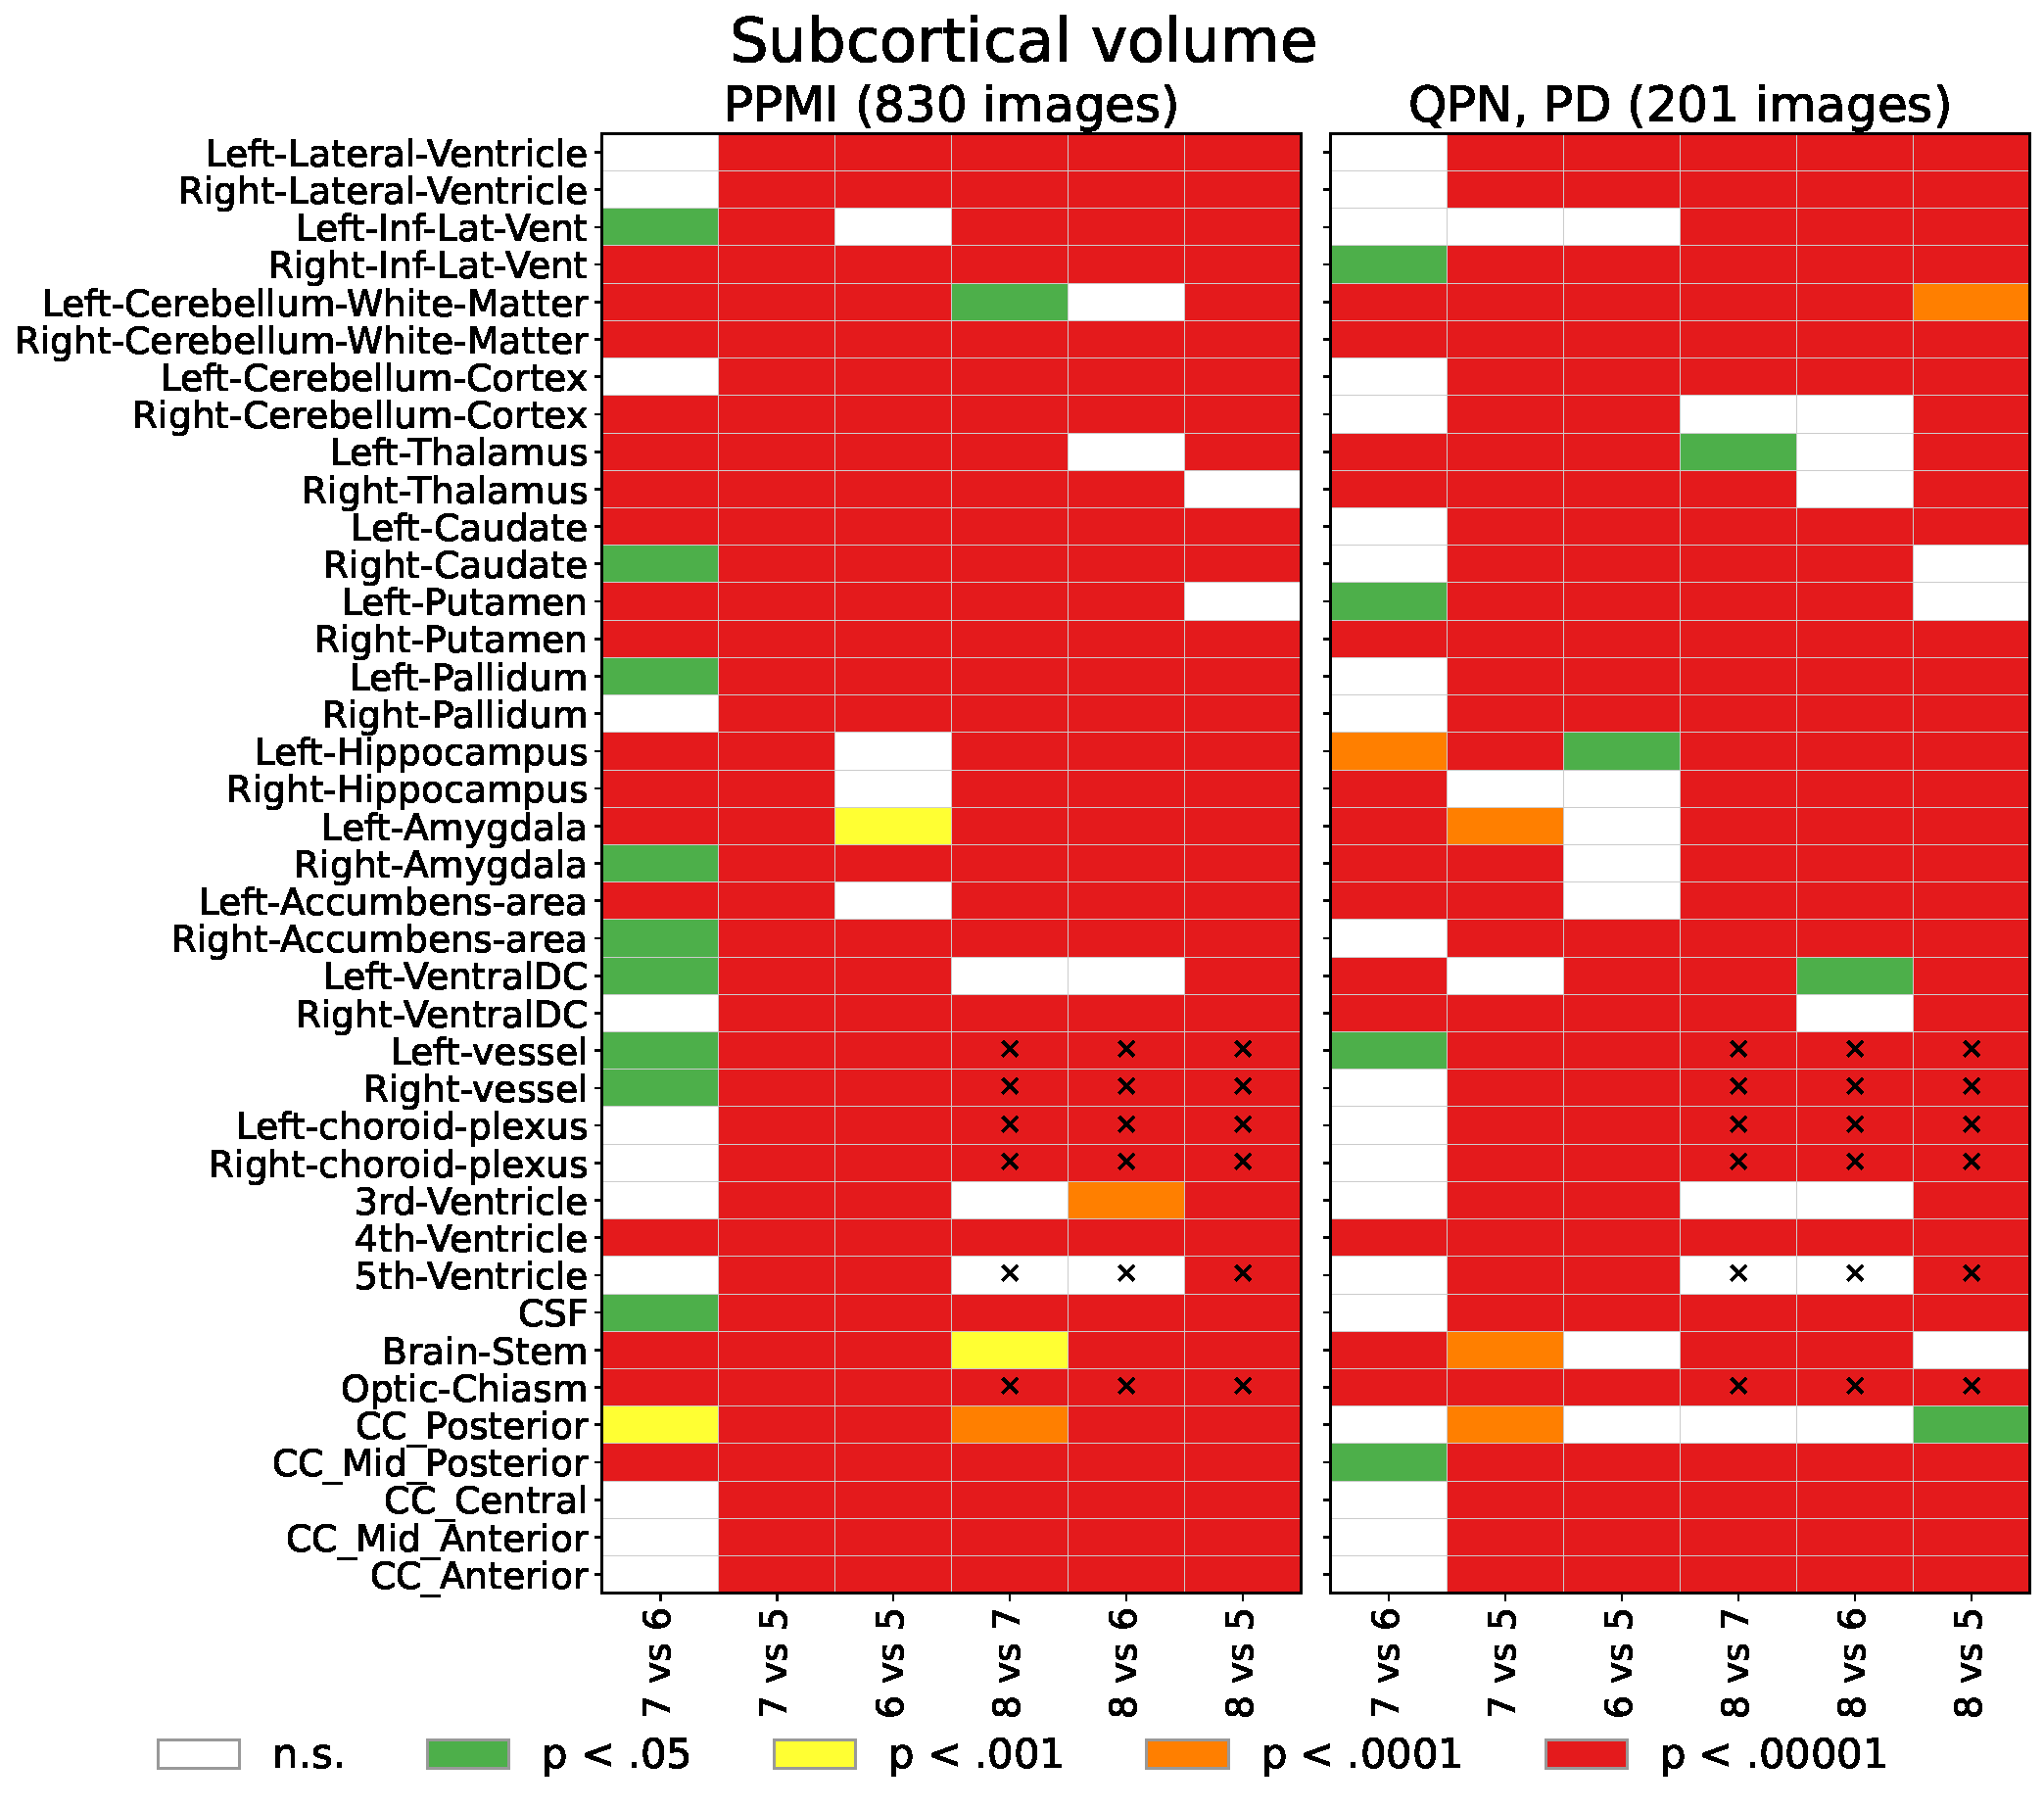
\includegraphics[height=0.55\textheight]{fig1_pvalues_subcortical}
\caption{Differences between FreeSurfer versions in estimation of subcortical volume \rev{in the PPMI sample (830
images, left) and in the PD patients of the QPN replication sample (right)}. Significant p-values reported in color, similar to the convention used in (Gronenschild et al., 2012).
p $<$ .05 in green, p $<$ .001 in yellow, p $<$ .0001 in orange, p $<$ .00001 in red, \rev{after Bonferroni
correction (thresholds divided by 187). $\times$, label not produced by FS8 (volume 0).} Segmentation with aseg
atlas implemented in FreeSurfer. Statistics are reported in Table S1 \rev{(PPMI) and S6 (QPN)}. PPMI, Parkinson's
Progression Markers Initiative; QPN, Quebec Parkinson Network.}\label{fig:1}
\end{figure}

\begin{figure}[H]
\centering
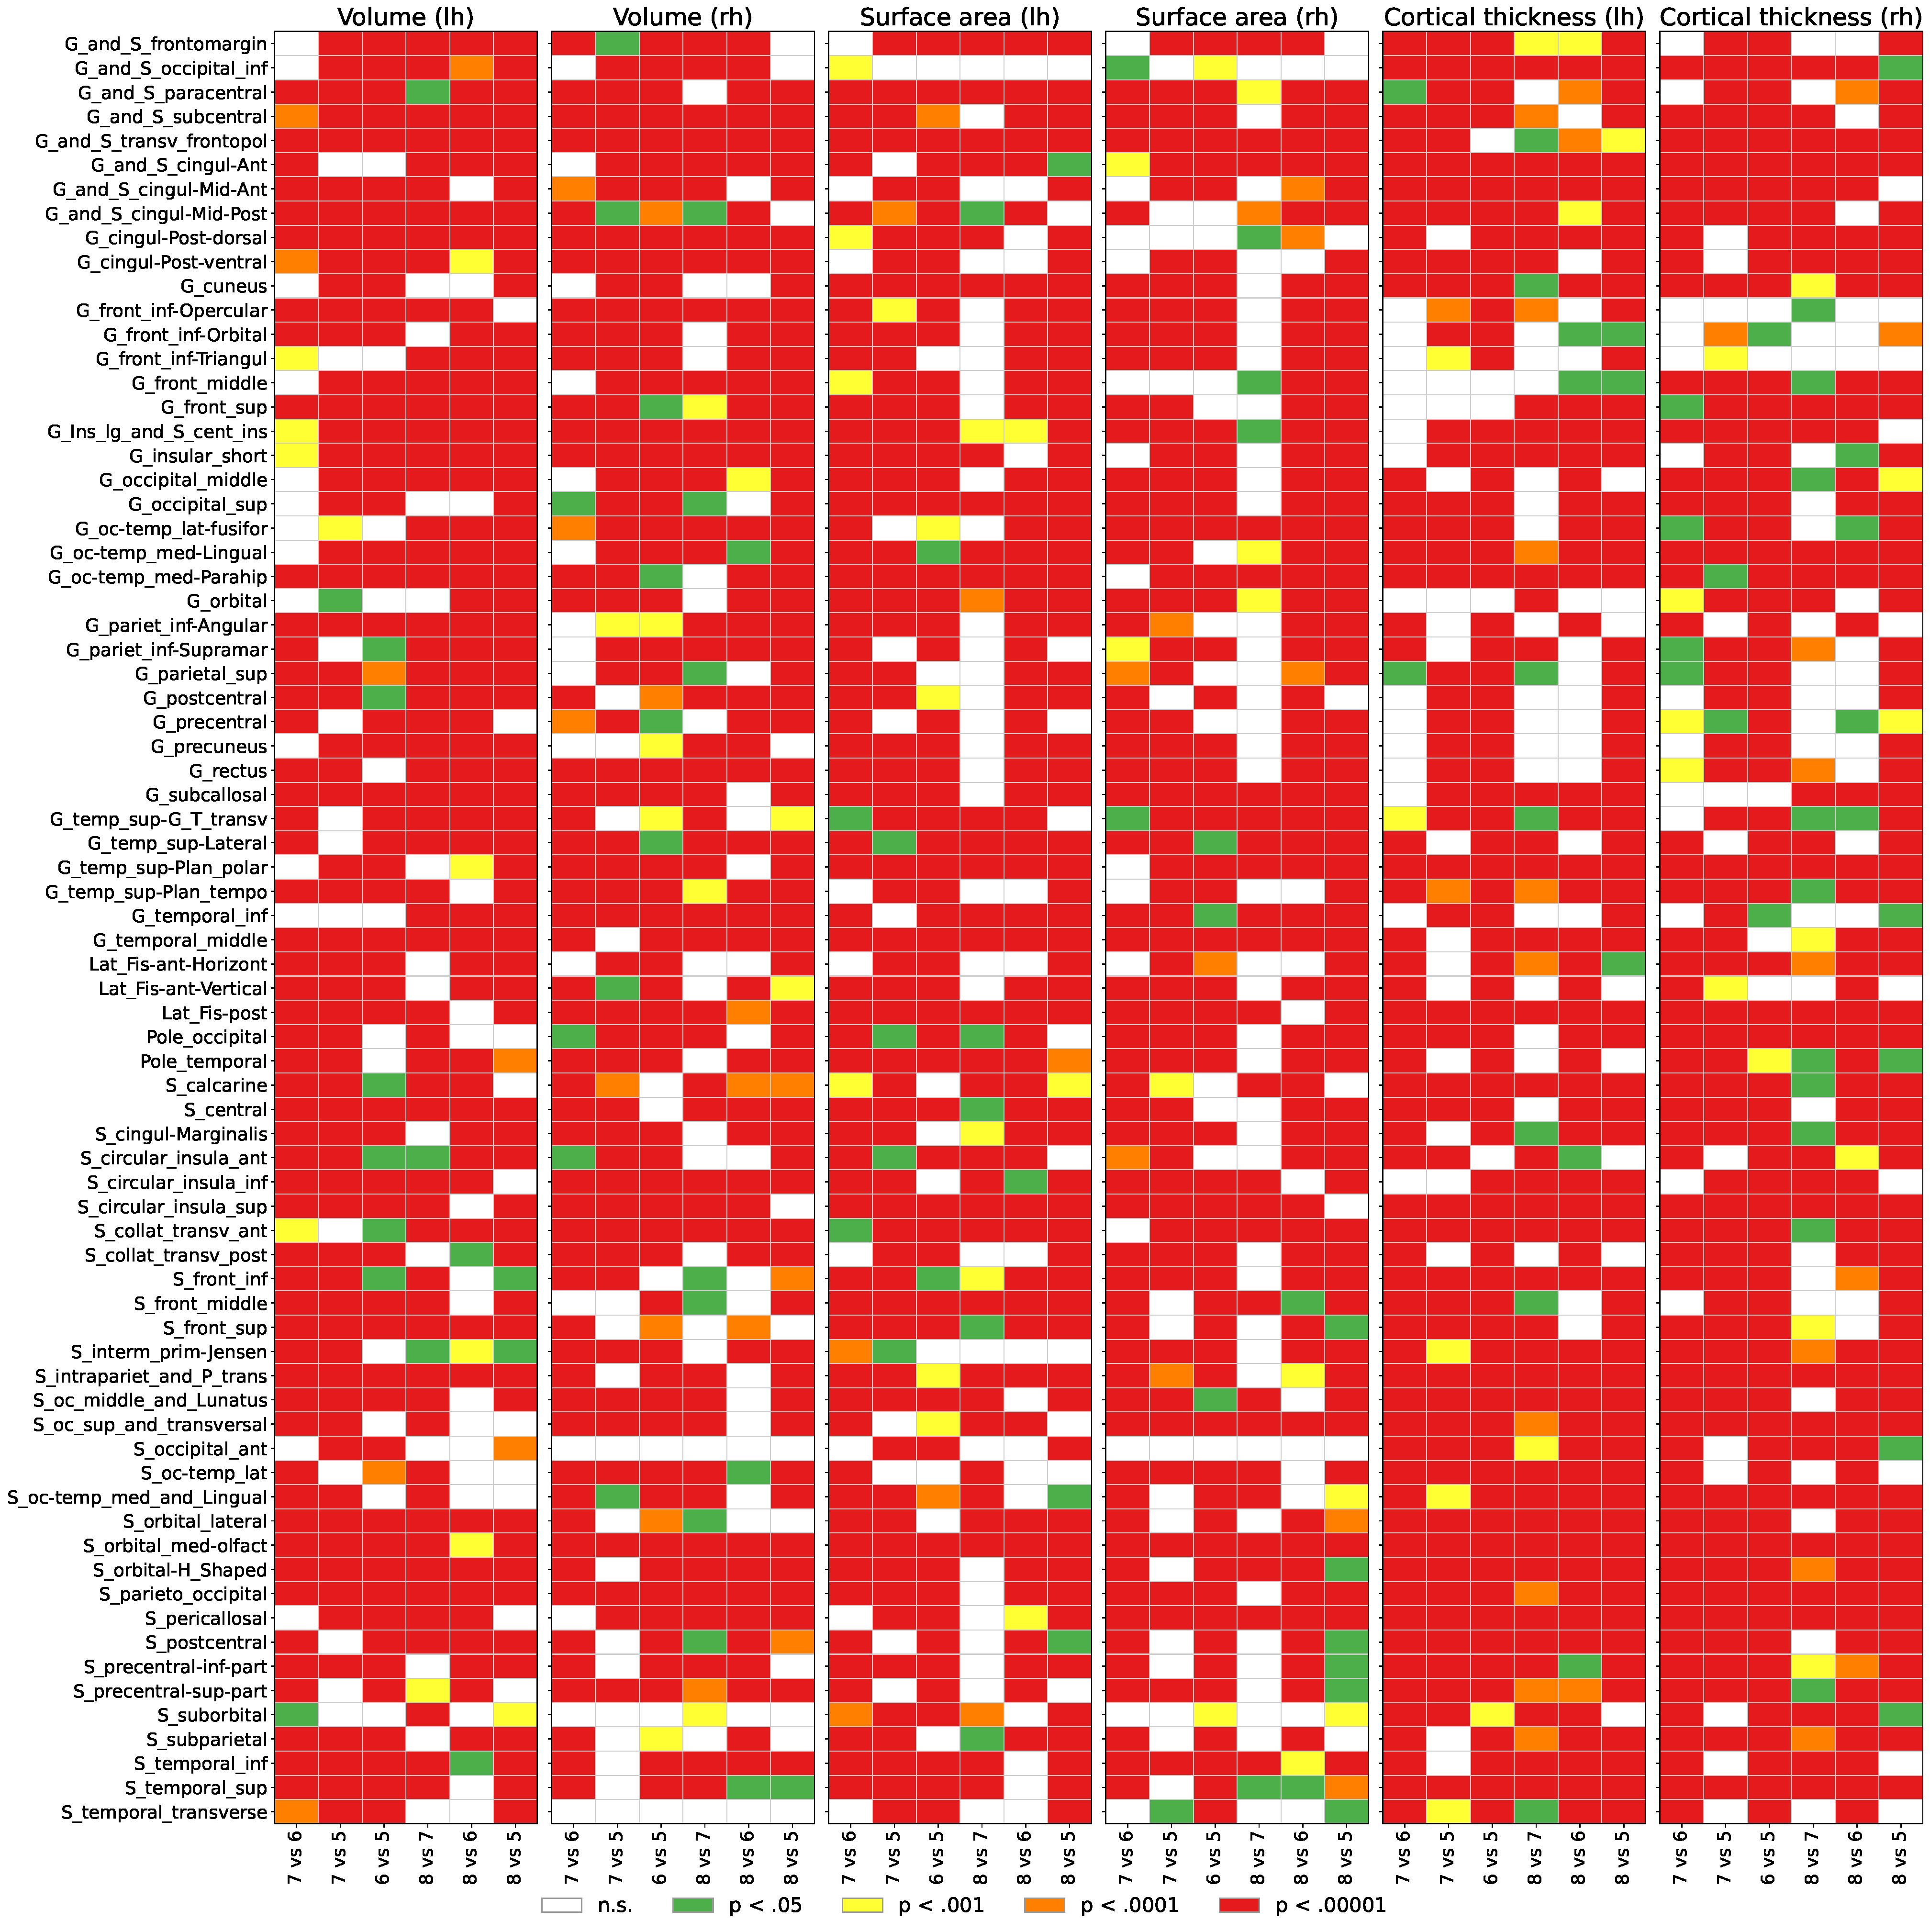
\includegraphics[width=\linewidth]{fig2_pvalues_cortical}
\caption{Differences between FreeSurfer versions in estimation of volume, surface area, and cortical thickness
\rev{in the PPMI sample (830 images)}. Significant p-values reported in color. p $<$ .05 in green, p $<$ .001 in
yellow, p $<$ .0001 in orange, p $<$ .00001 in red, \rev{after Bonferroni correction (thresholds divided by 187
for volume and 148 for surface area and thickness)}. Parcellation with Destrieux atlas implemented in FreeSurfer.
Statistics are reported in Table \rev{S1 (PPMI) and S6 (QPN)}. lh, left hemisphere; rh, right hemisphere. PPMI,
Parkinson's Progression Markers Initiative; QPN, Quebec Parkinson Network.}\label{fig:2}
\end{figure}

Estimation of volumes, surface areas, and cortical thickness across the \rev{four} FreeSurfer versions are
represented in Figures \rev{S1 and S2}. Between and within-subject variability is represented in
Figures~\ref{fig:3}--\ref{fig:6}. For certain regions, the differences in the estimation of structural measures are
higher for two different subjects analyzed by the same FS version than for the same subject when analyzed by two
different FS versions. For example, the left hippocampus had higher between-subject variability than
between-version variability (see Figure~\ref{fig:3}). These variabilities were visualized in Figure \rev{S3}. The
shapes and overlap between hippocampi in two different subjects seem to differ more than in the same subject
varying in the software version. This suggests that the volume itself may not be the best metric to measure
software variability. \rev{The overlap of the segmentations between versions is reported in Figure S4.}

\begin{figure}[H]
\centering
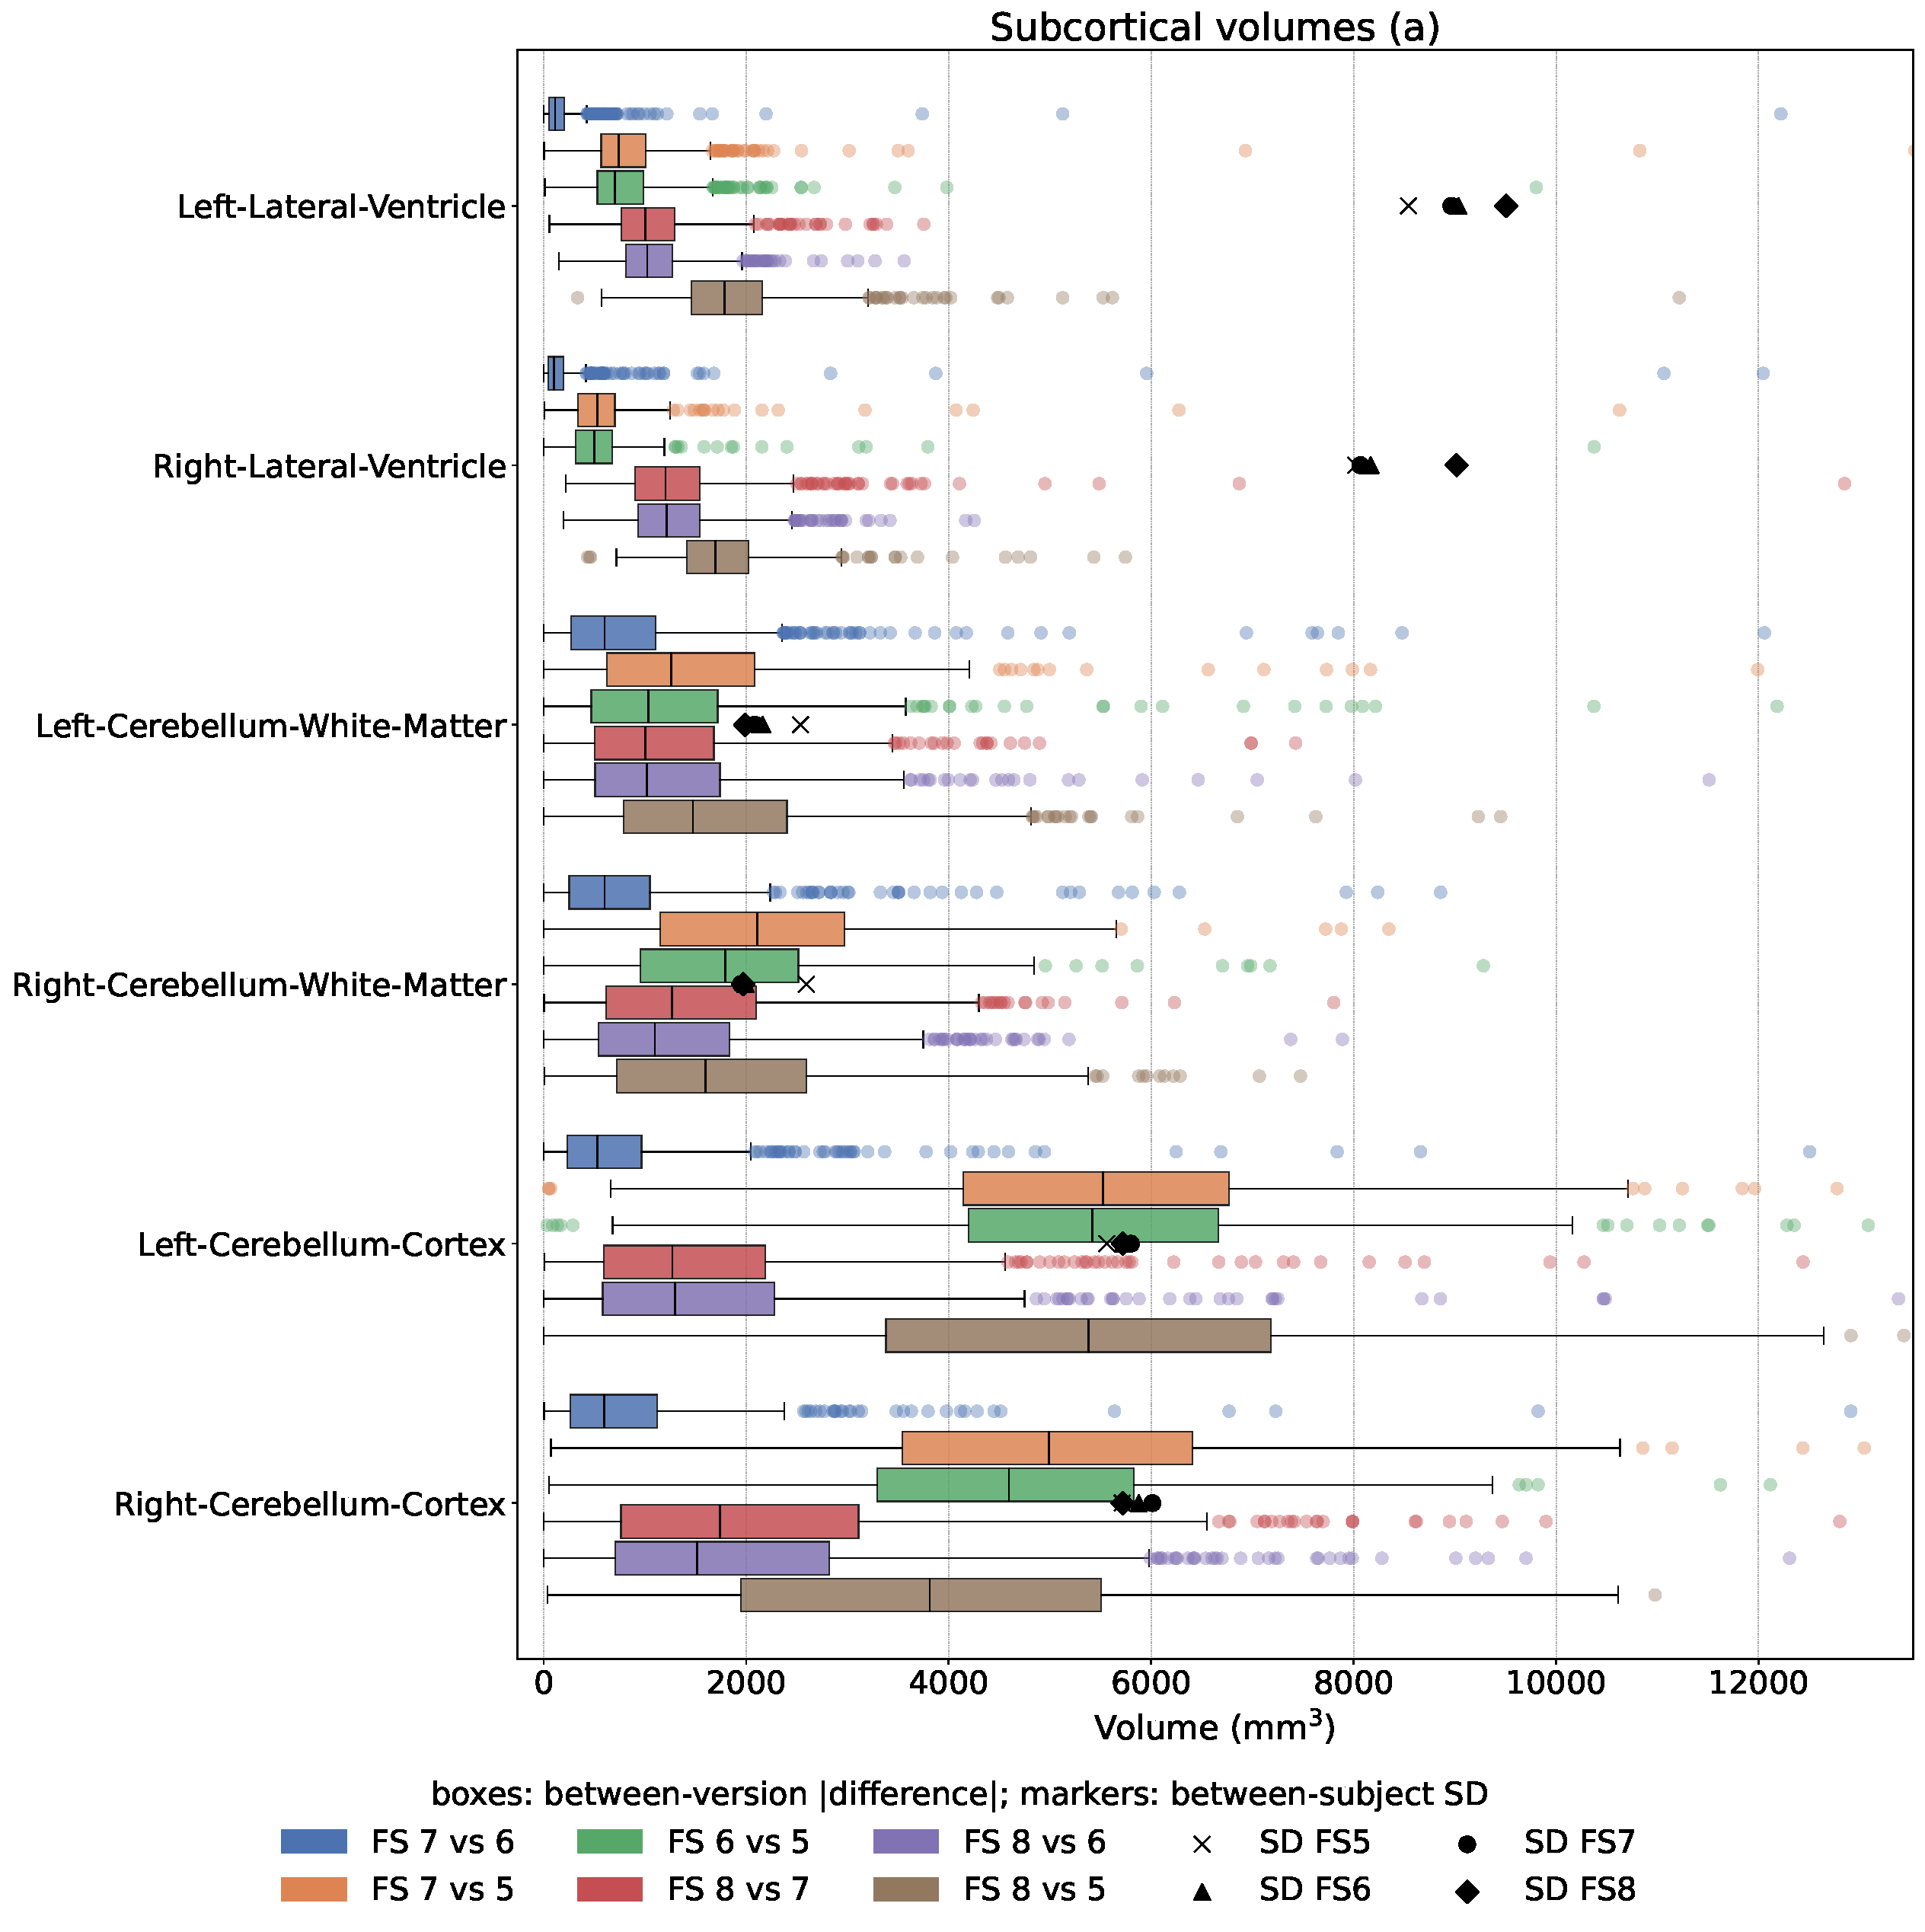
\includegraphics[width=\linewidth,height=0.8\textheight,keepaspectratio]{variability_subcortical_part1}
\caption{Between-version (\rev{n = 6 version pairs}) and between-subject (\rev{n = 830 images}) subcortical
volume variability\rev{, (a) lateral ventricles and cerebellum (white matter and cortex), (b) other structures,
on separate axes because their variability is an order of magnitude larger}. Absolute difference between FreeSurfer
versions represented as colored box plots, standard deviations \rev{of each version} represented as black
markers. \rev{Outliers beyond the x-axis range are not shown.}}\label{fig:3}
\end{figure}

\begin{figure}[H]
\ContinuedFloat
\centering
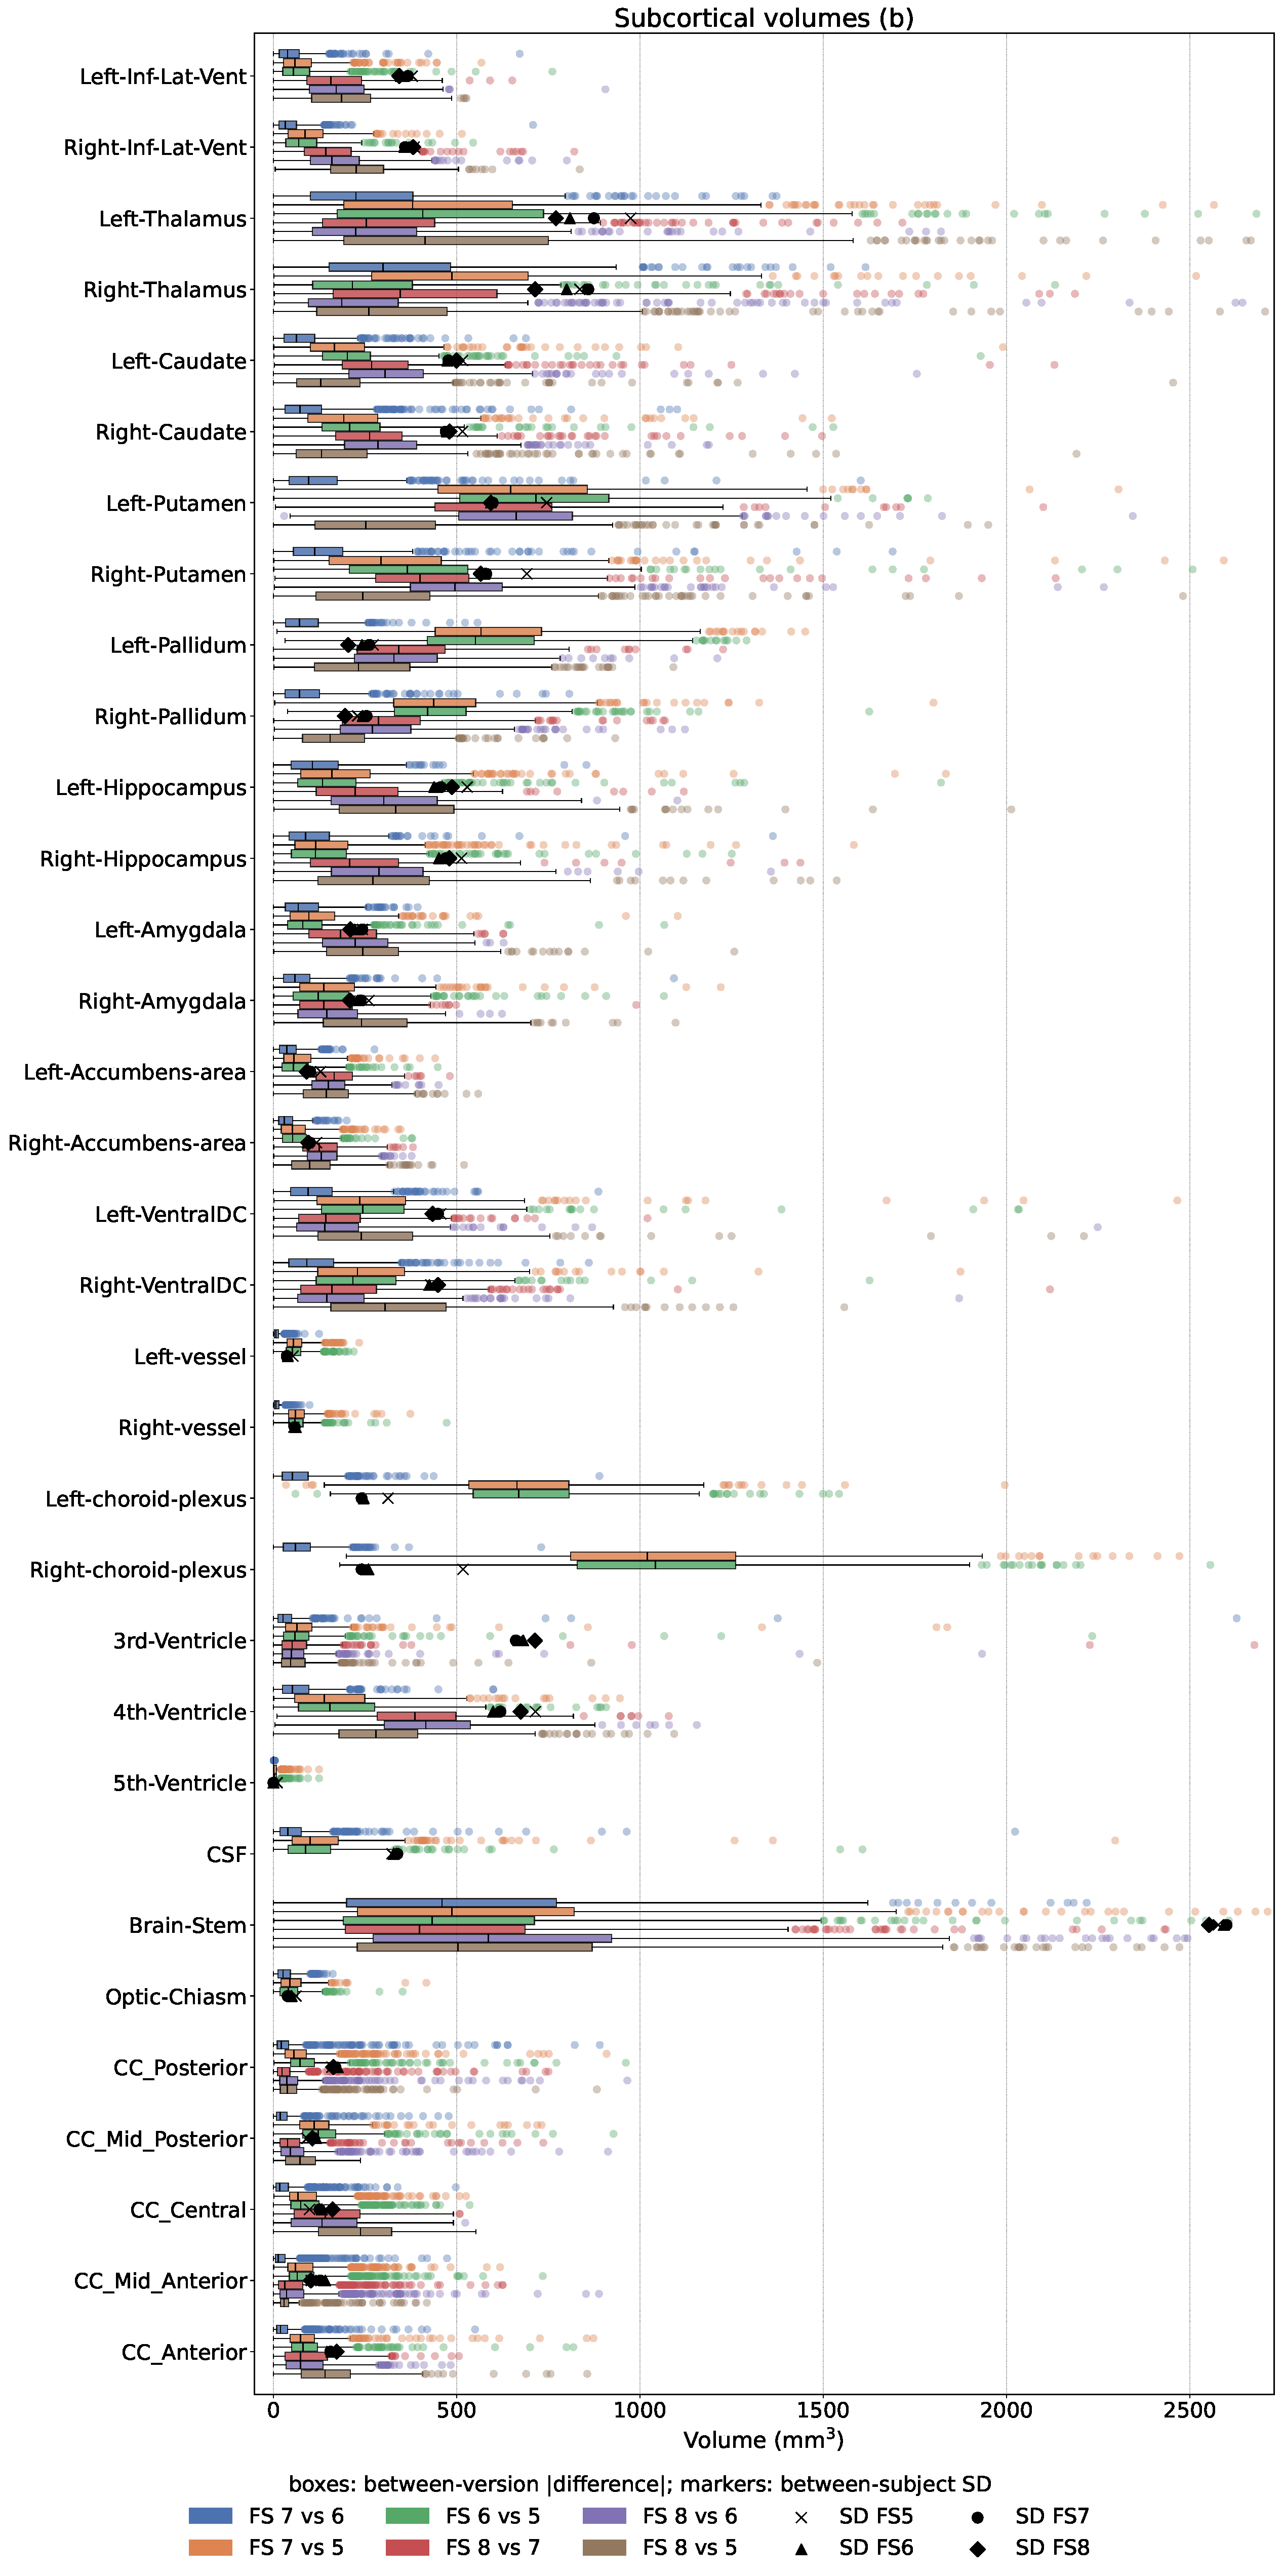
\includegraphics[width=\linewidth,height=0.85\textheight,keepaspectratio]{variability_subcortical_part2}
\caption{\rev{(continued) (b) Other subcortical structures.}}
\end{figure}

\begin{figure}[H]
\centering
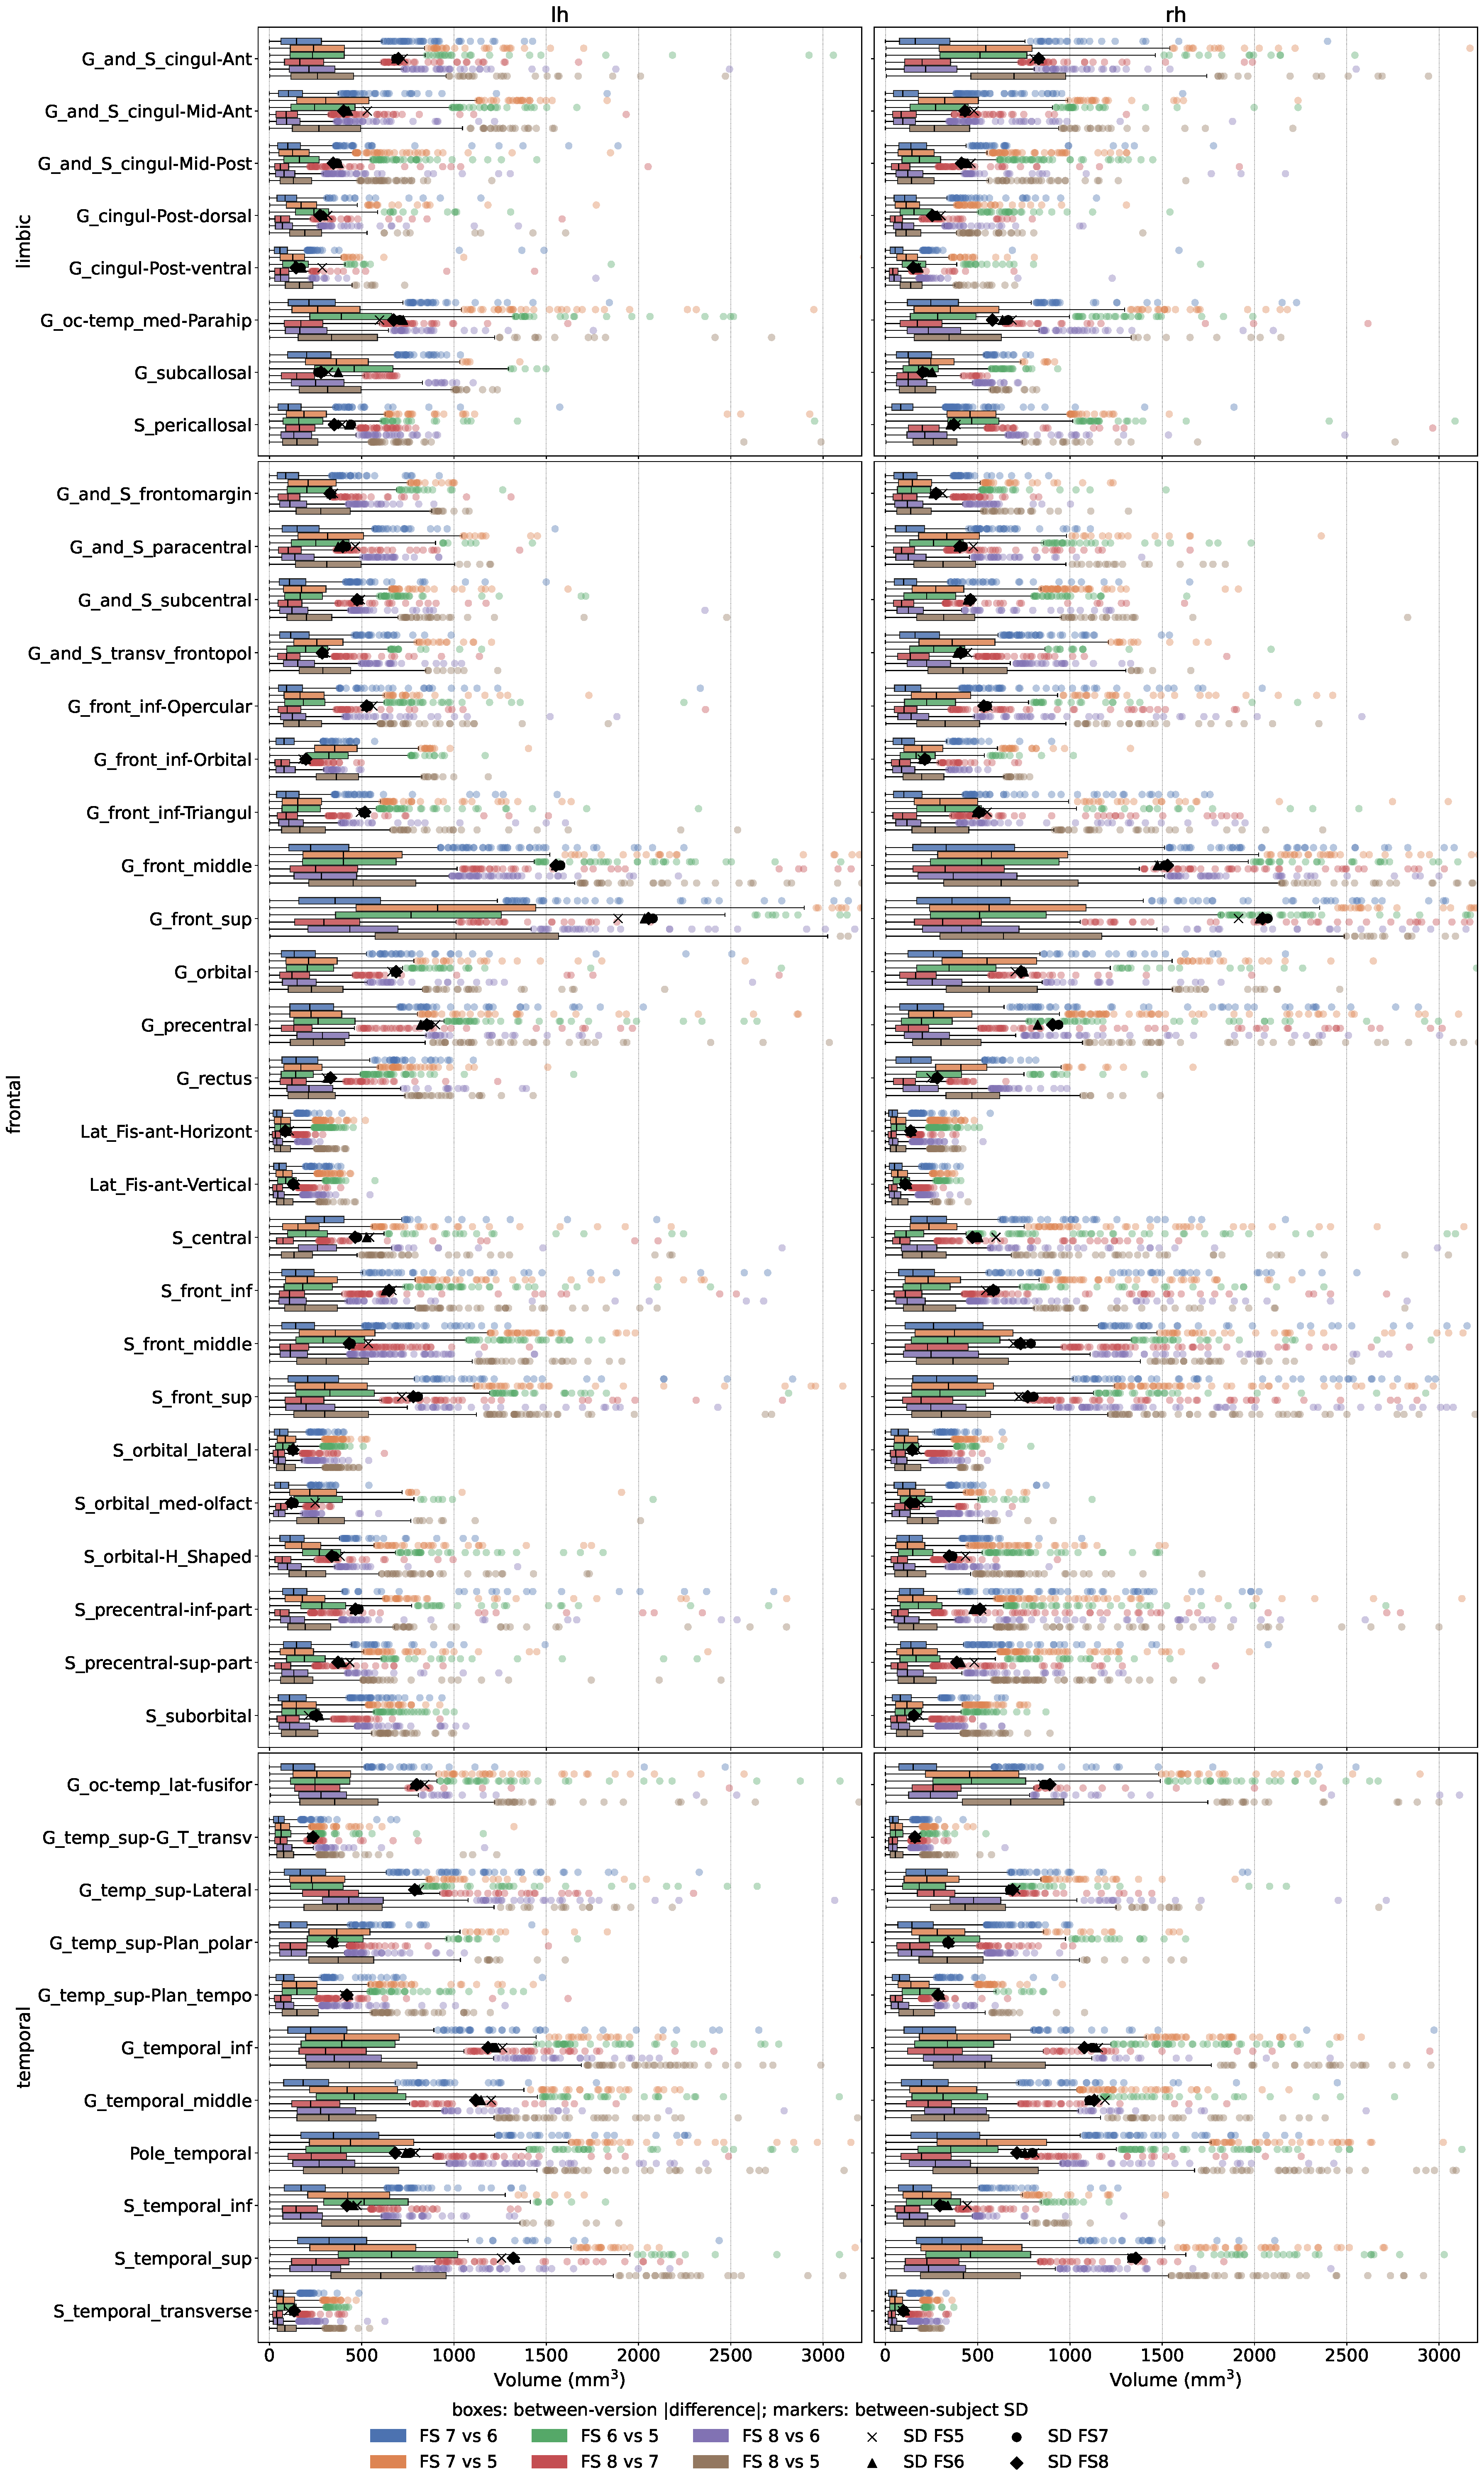
\includegraphics[width=\linewidth,height=0.8\textheight,keepaspectratio]{variability_vol_part1}
\caption{Between-version (\rev{n = 6 version pairs}) and between-subject (\rev{n = 830 images}) cortical volume
variability \rev{in the left (left panels) and right (right panels) hemispheres, (a) limbic, frontal and temporal
regions, (b) occipital, parietal and other regions; outliers beyond the x-axis range are not shown}. Absolute difference between
FreeSurfer versions represented as box plots, standard deviations \rev{of each version} represented as black
markers.}\label{fig:4}
\end{figure}

\begin{figure}[H]
\ContinuedFloat
\centering
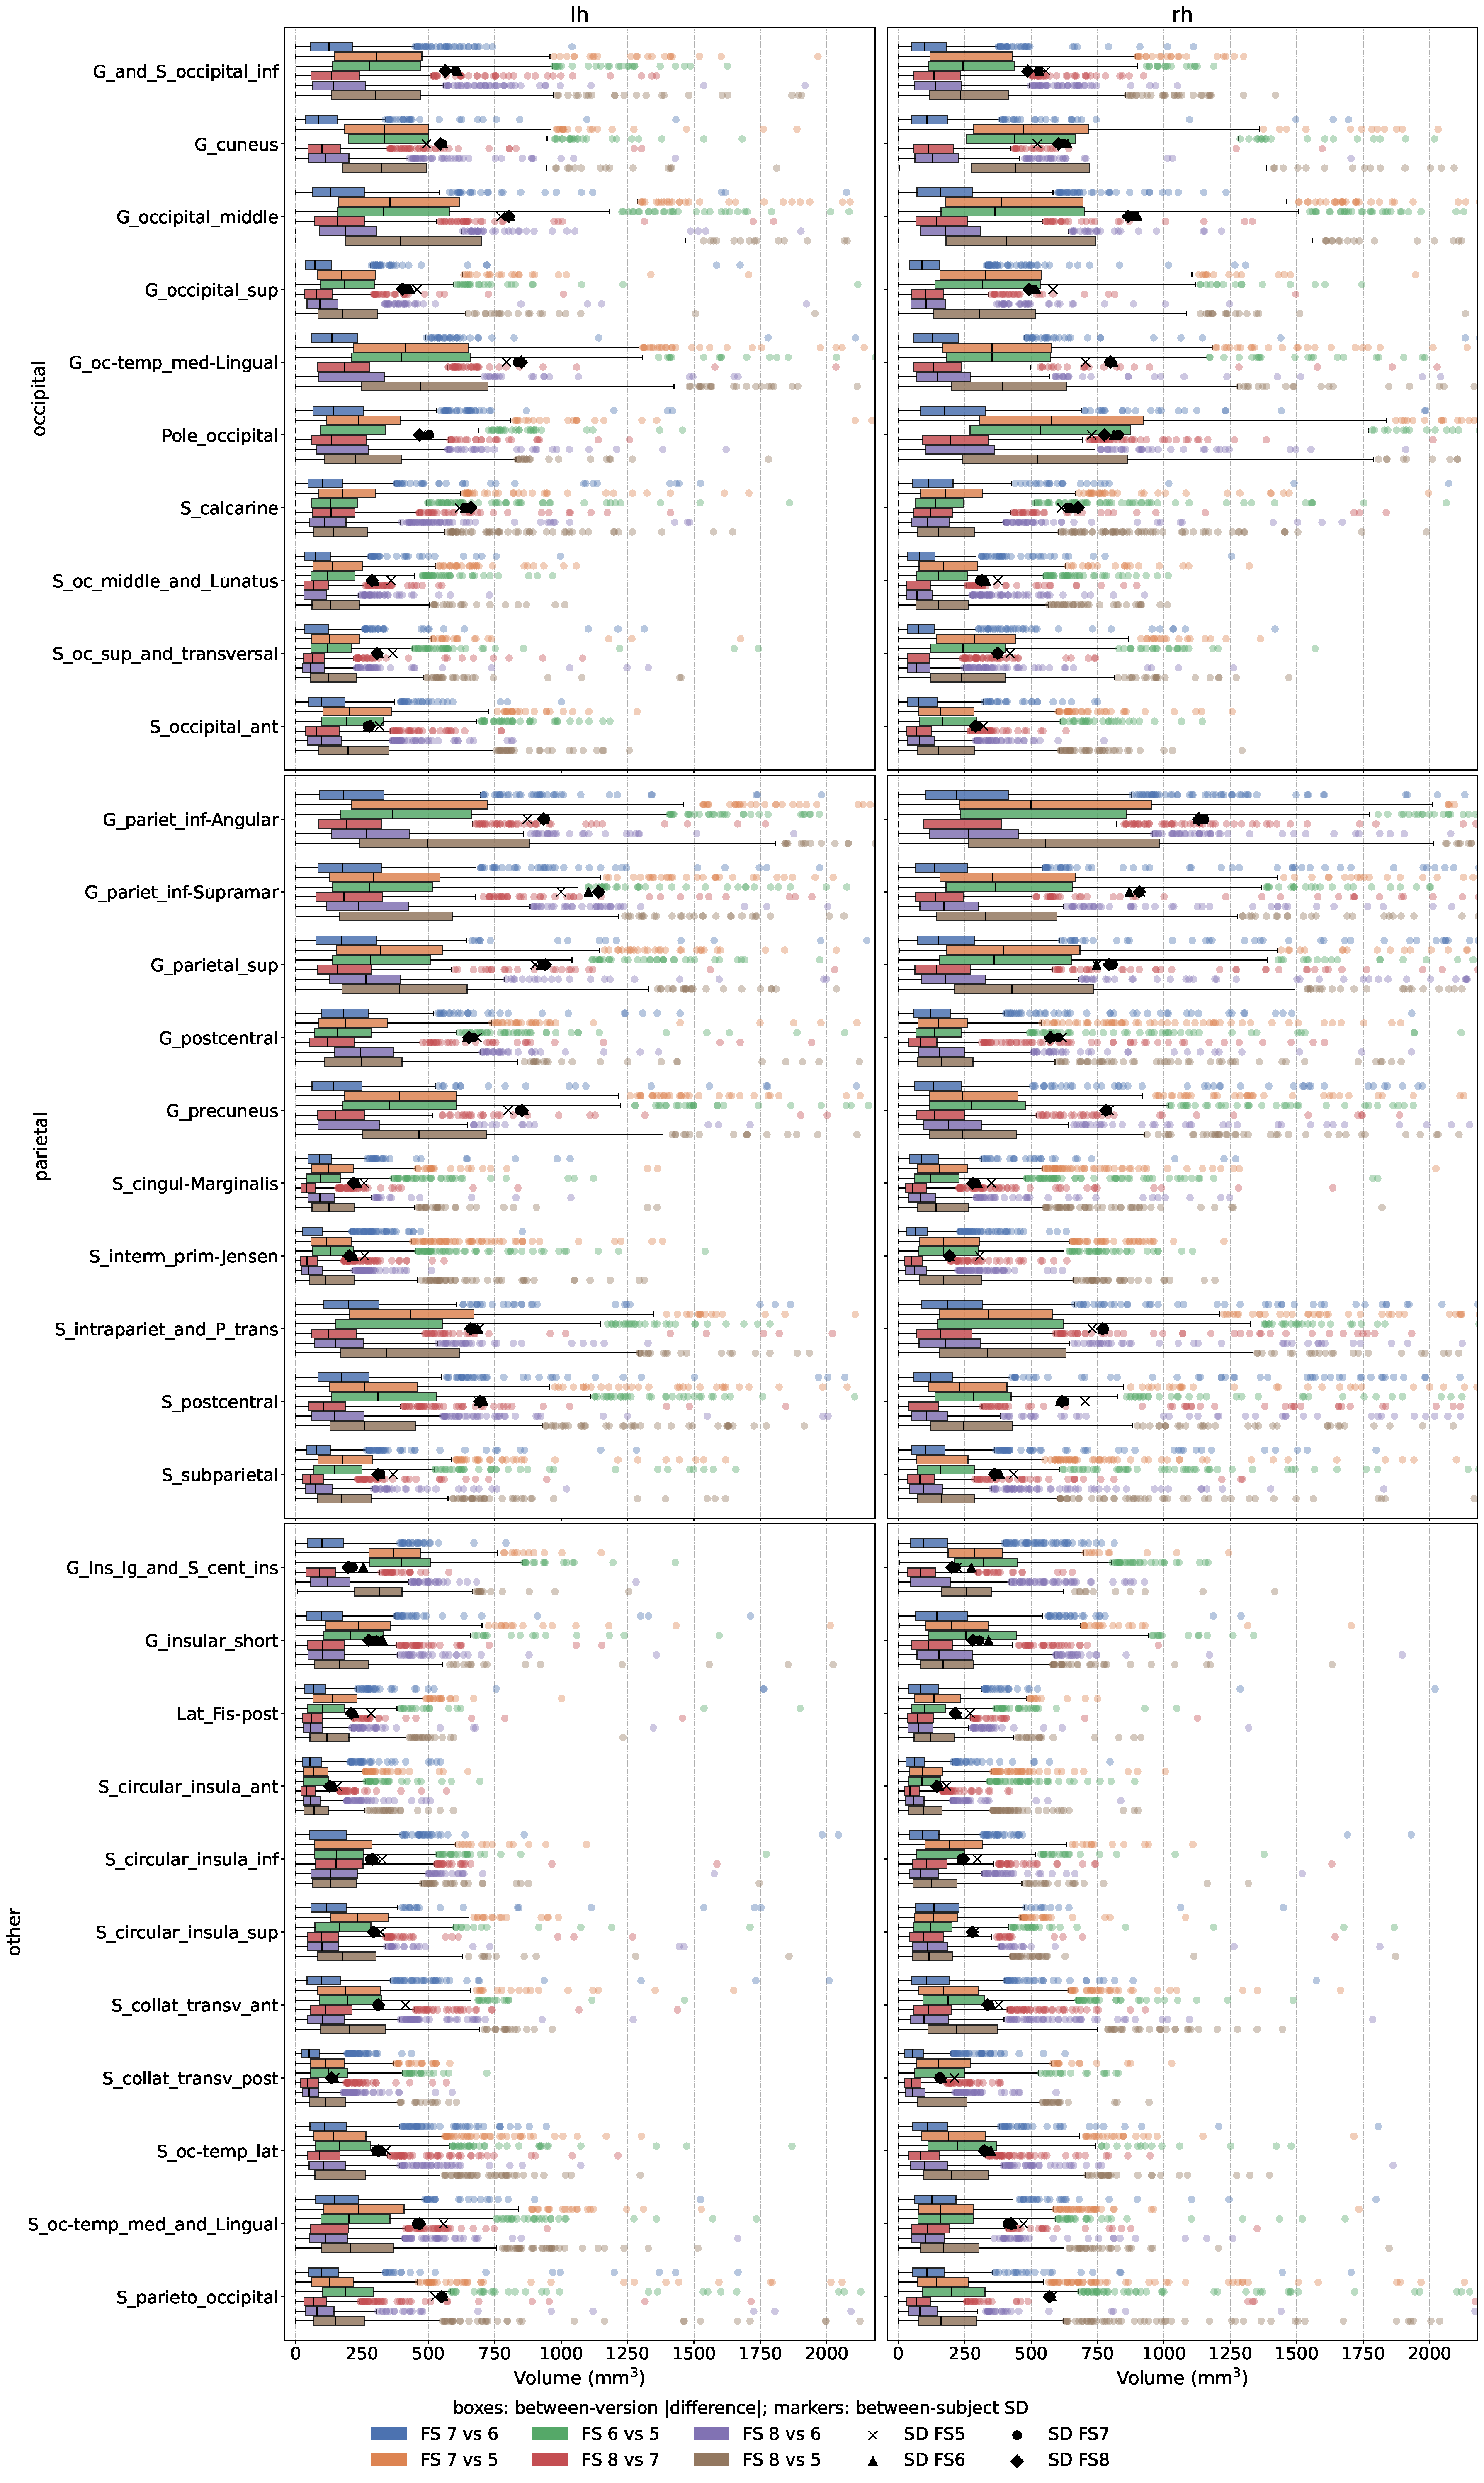
\includegraphics[width=\linewidth,height=0.8\textheight,keepaspectratio]{variability_vol_part2}
\caption{\rev{(continued) (b) Occipital, parietal and other regions.}}
\end{figure}

\begin{figure}[H]
\centering
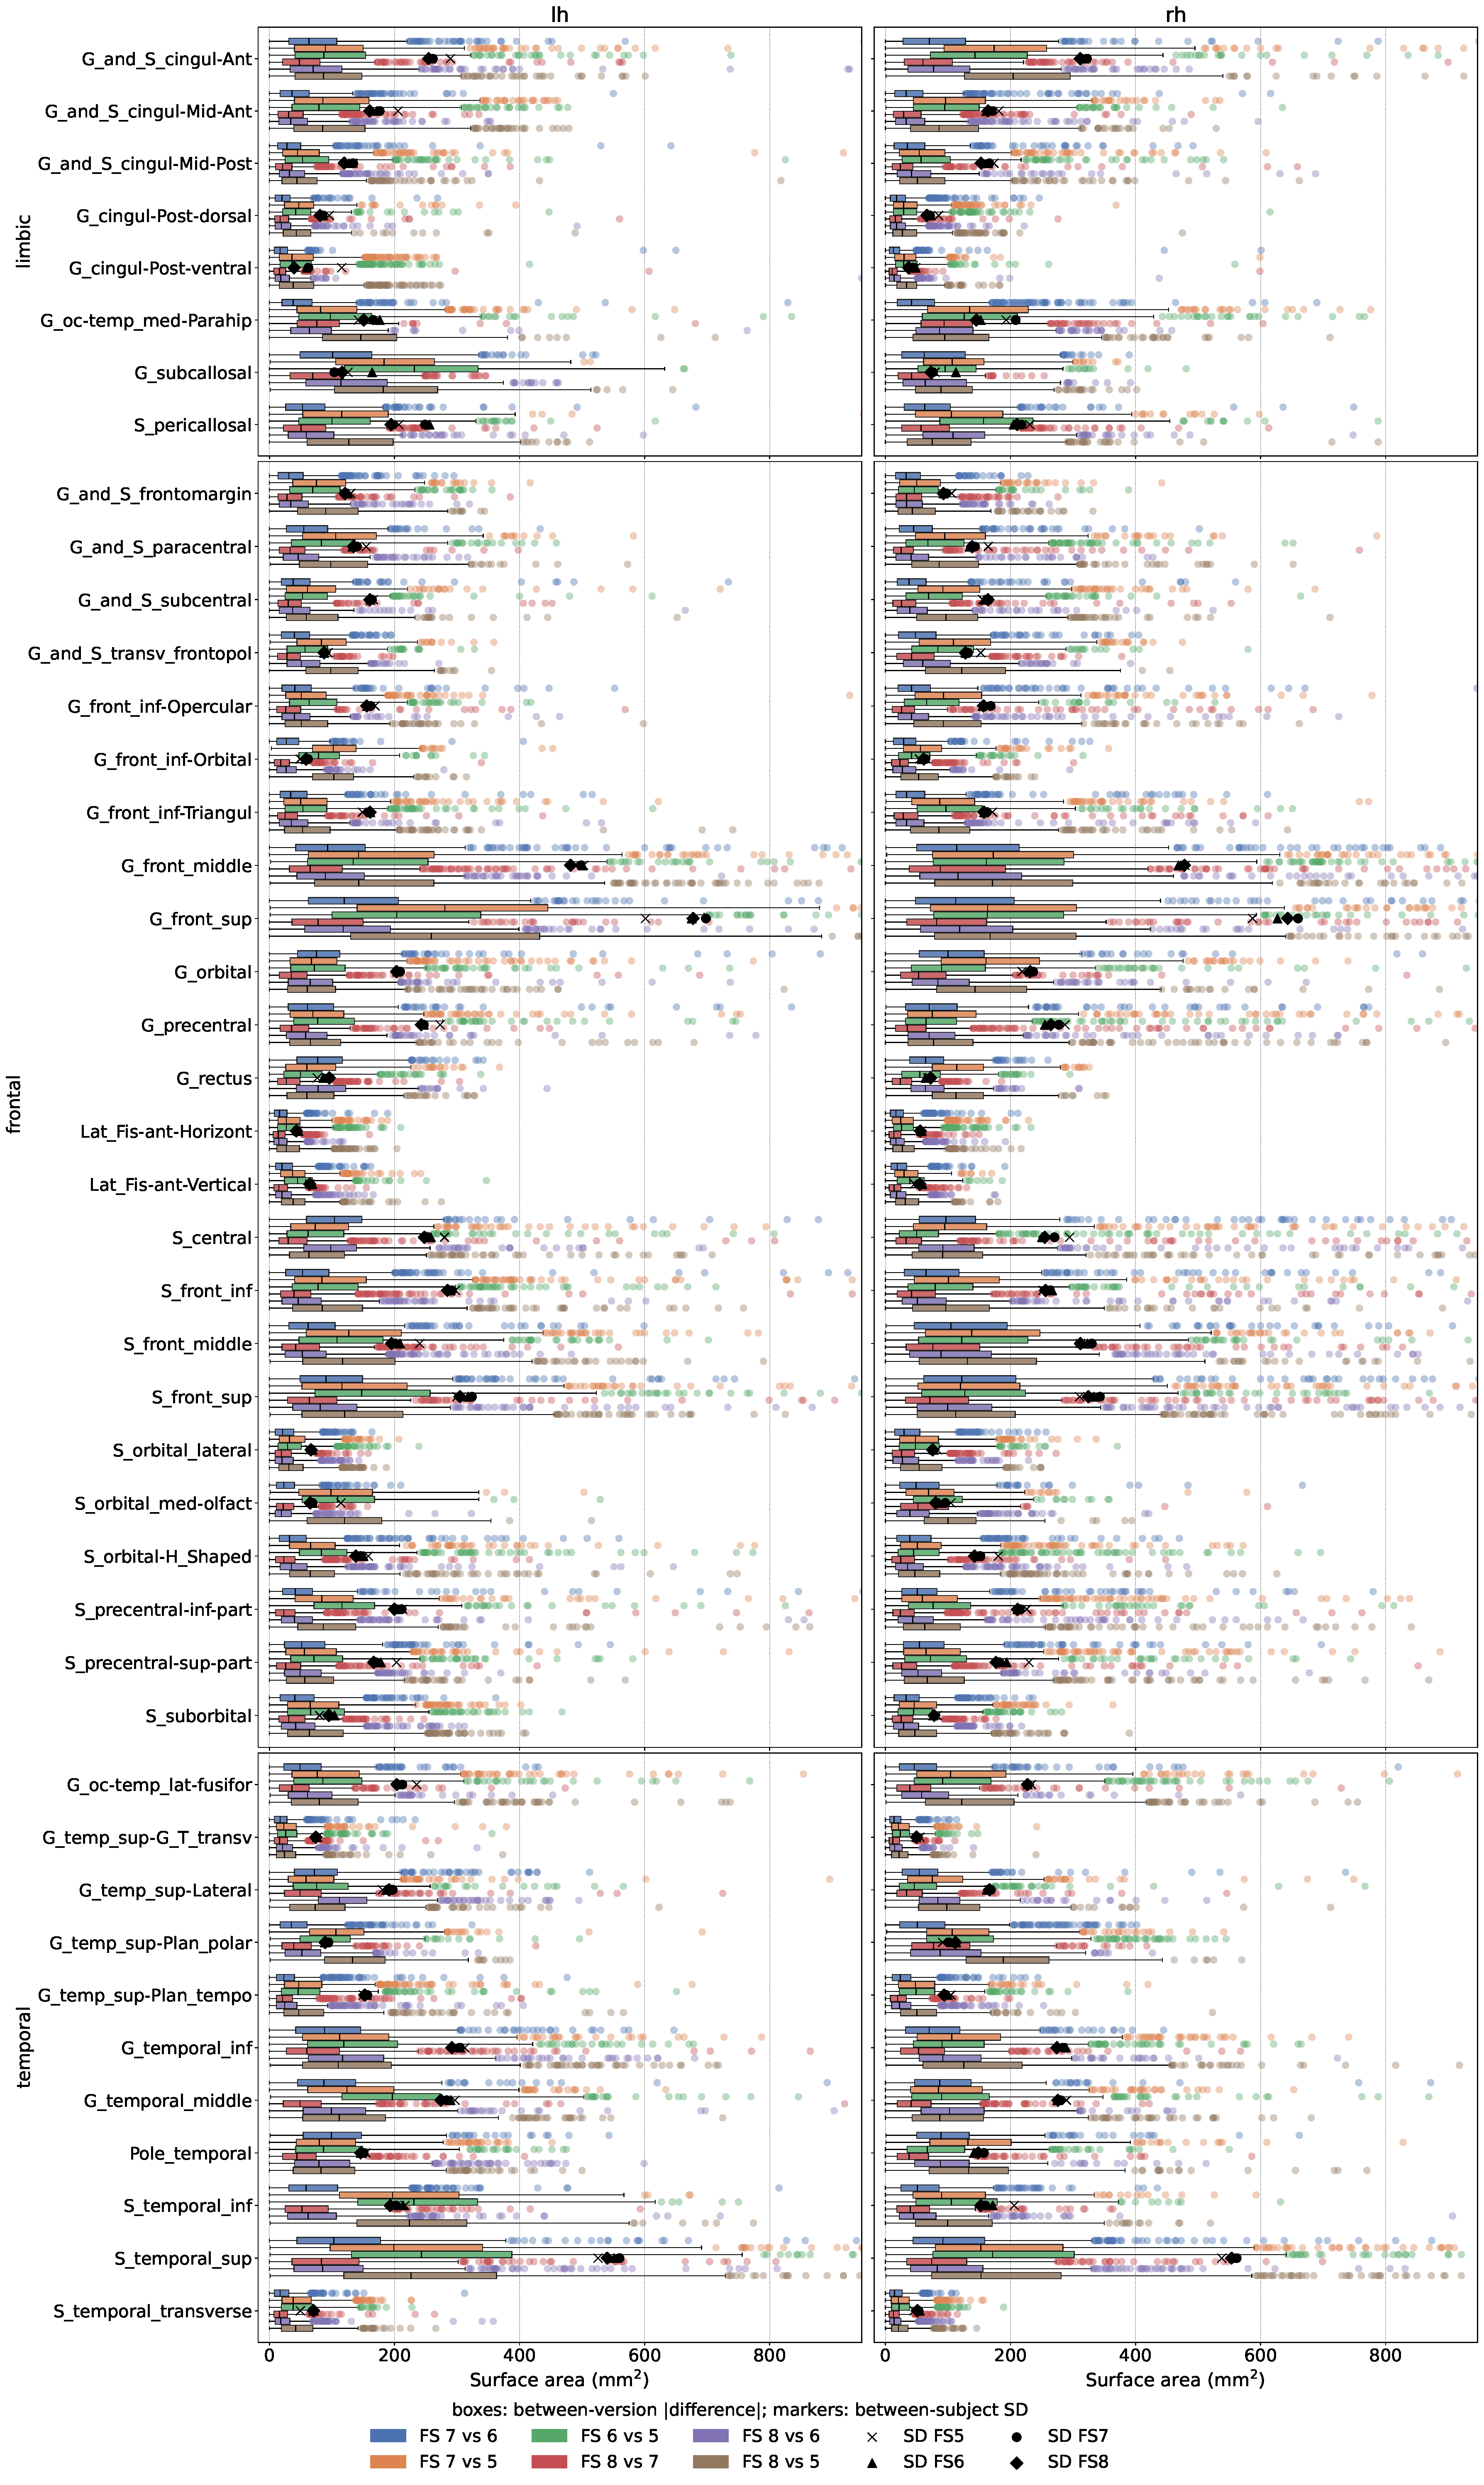
\includegraphics[width=\linewidth,height=0.8\textheight,keepaspectratio]{variability_surf_part1}
\caption{Between-version (\rev{n = 6 version pairs}) and between-subject (\rev{n = 830 images}) surface area
variability \rev{in the left and right hemispheres, (a) limbic, frontal and temporal regions, (b) occipital,
parietal and other regions; outliers beyond the x-axis range are not shown}. Absolute difference between FreeSurfer versions represented as
box plots, standard deviations \rev{of each version} represented as black markers.}\label{fig:5}
\end{figure}

\begin{figure}[H]
\ContinuedFloat
\centering
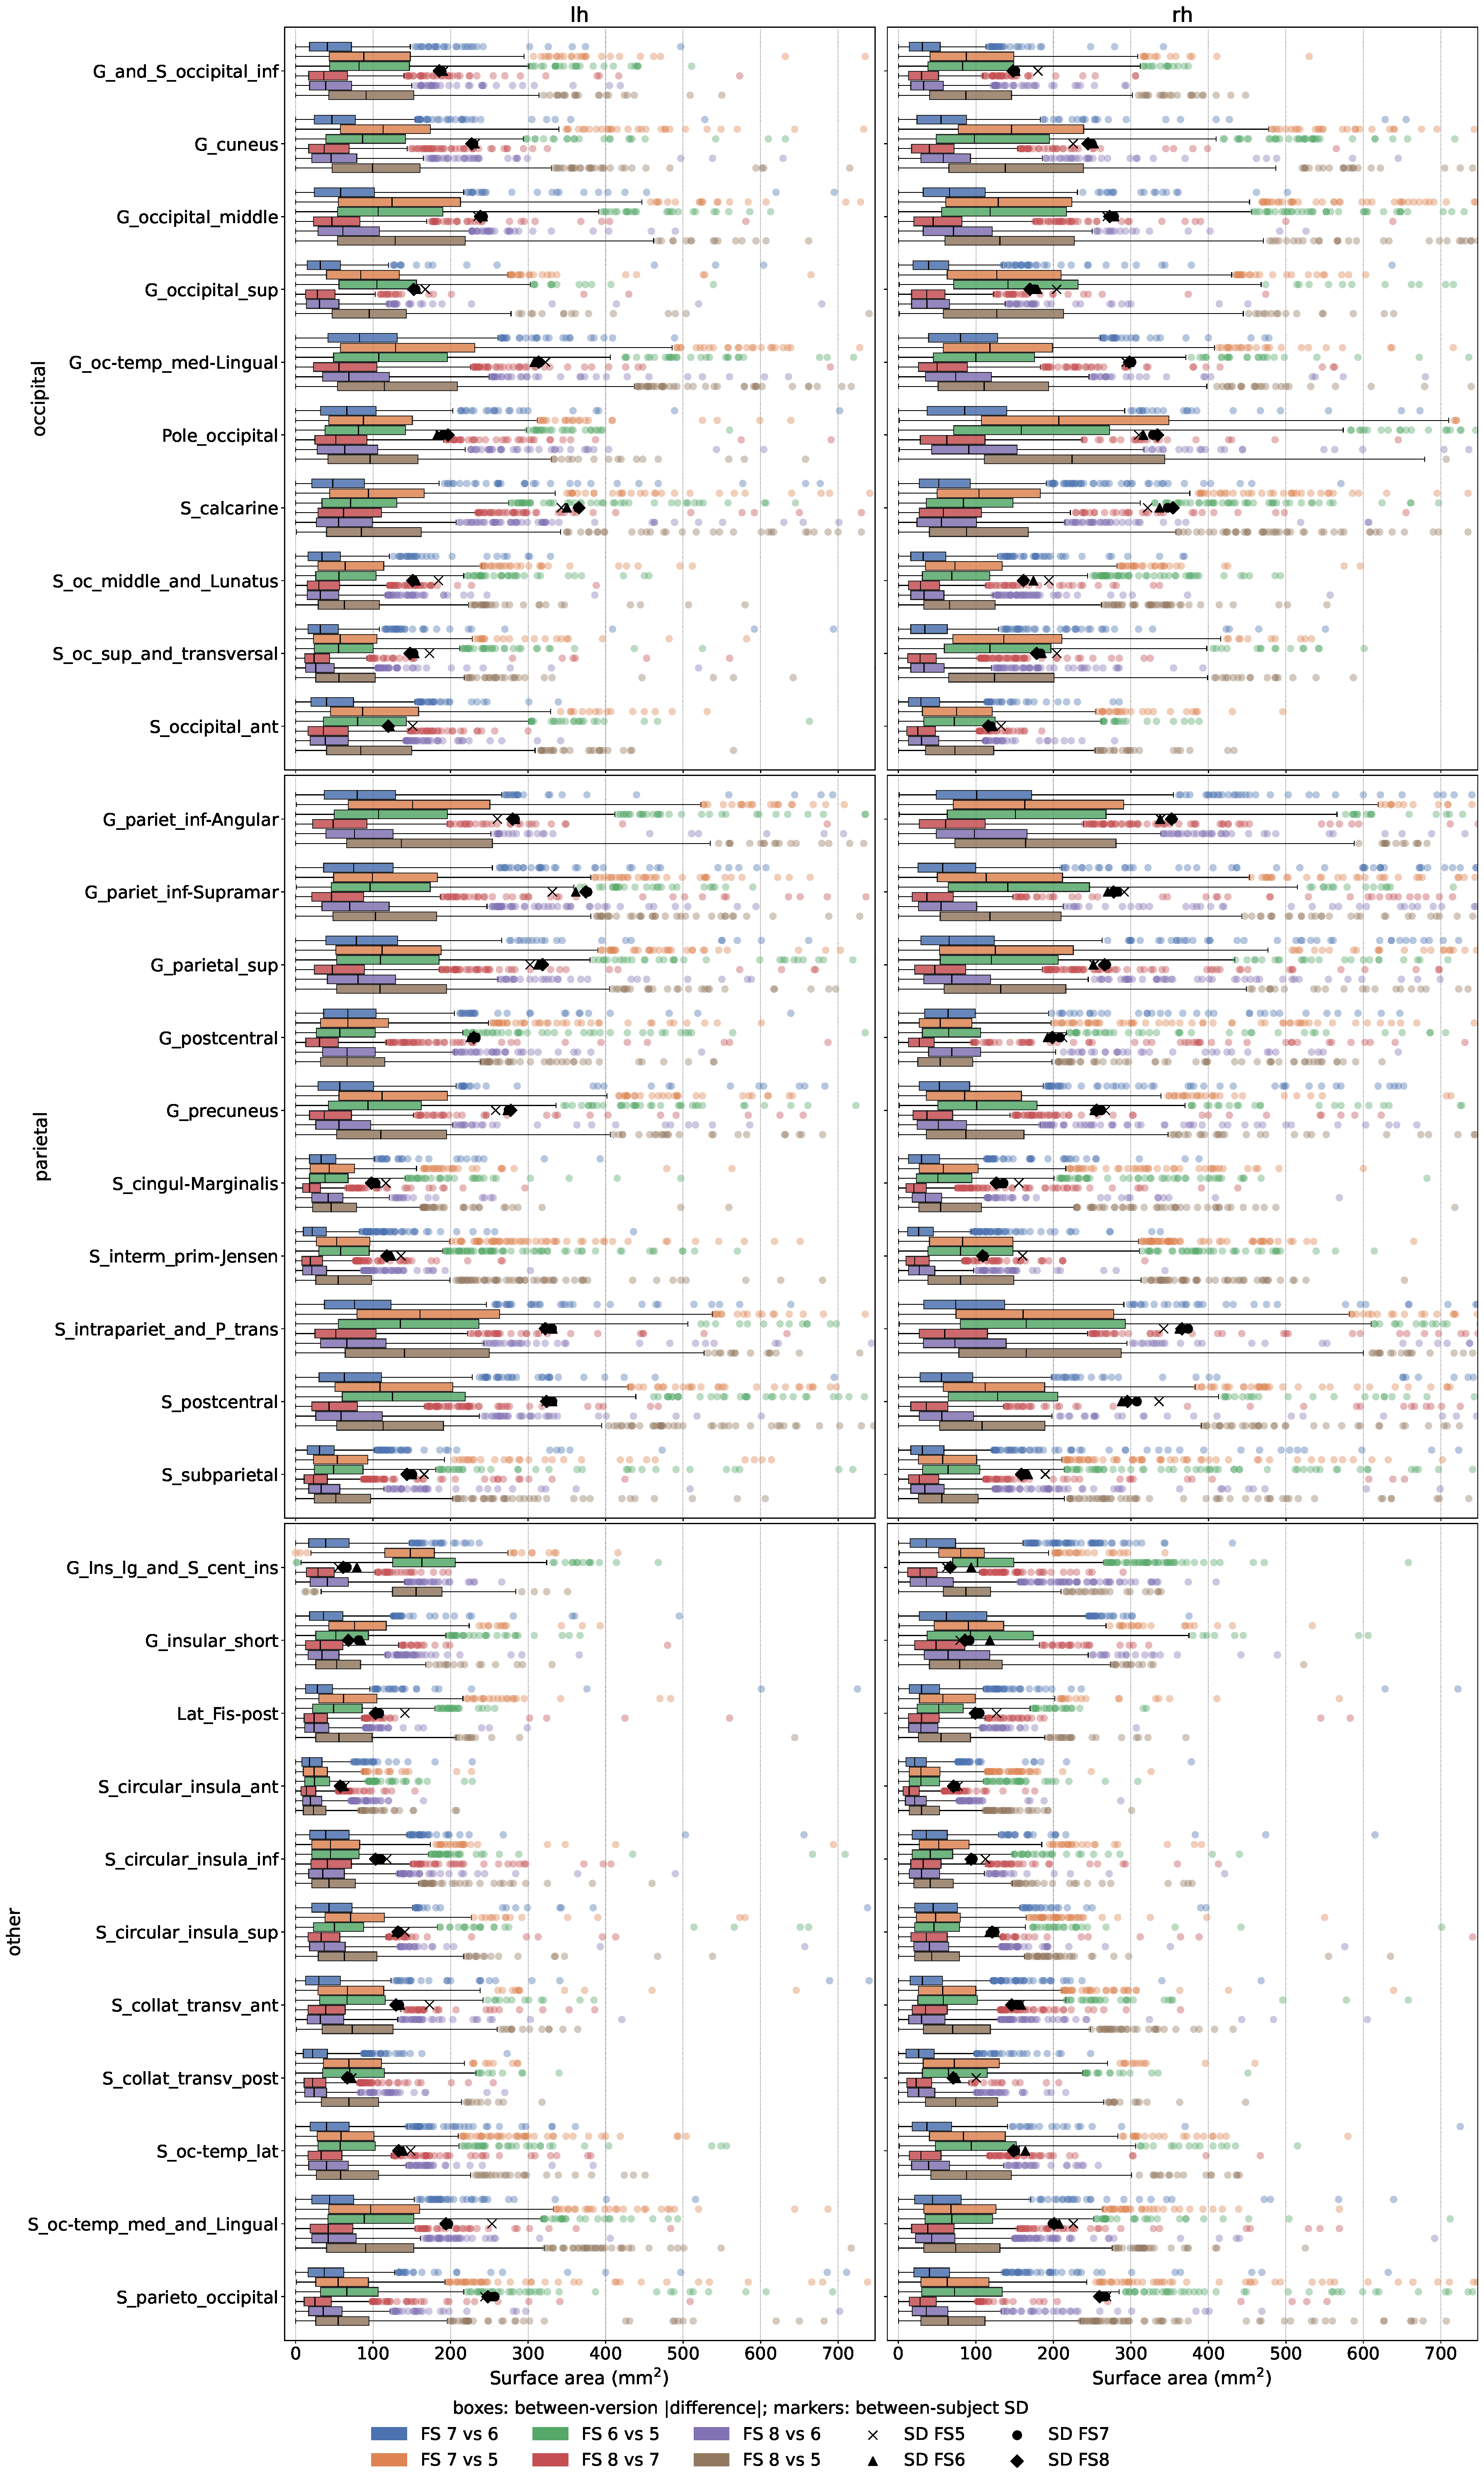
\includegraphics[width=\linewidth,height=0.8\textheight,keepaspectratio]{variability_surf_part2}
\caption{\rev{(continued) (b) Occipital, parietal and other regions.}}
\end{figure}

\begin{figure}[H]
\centering
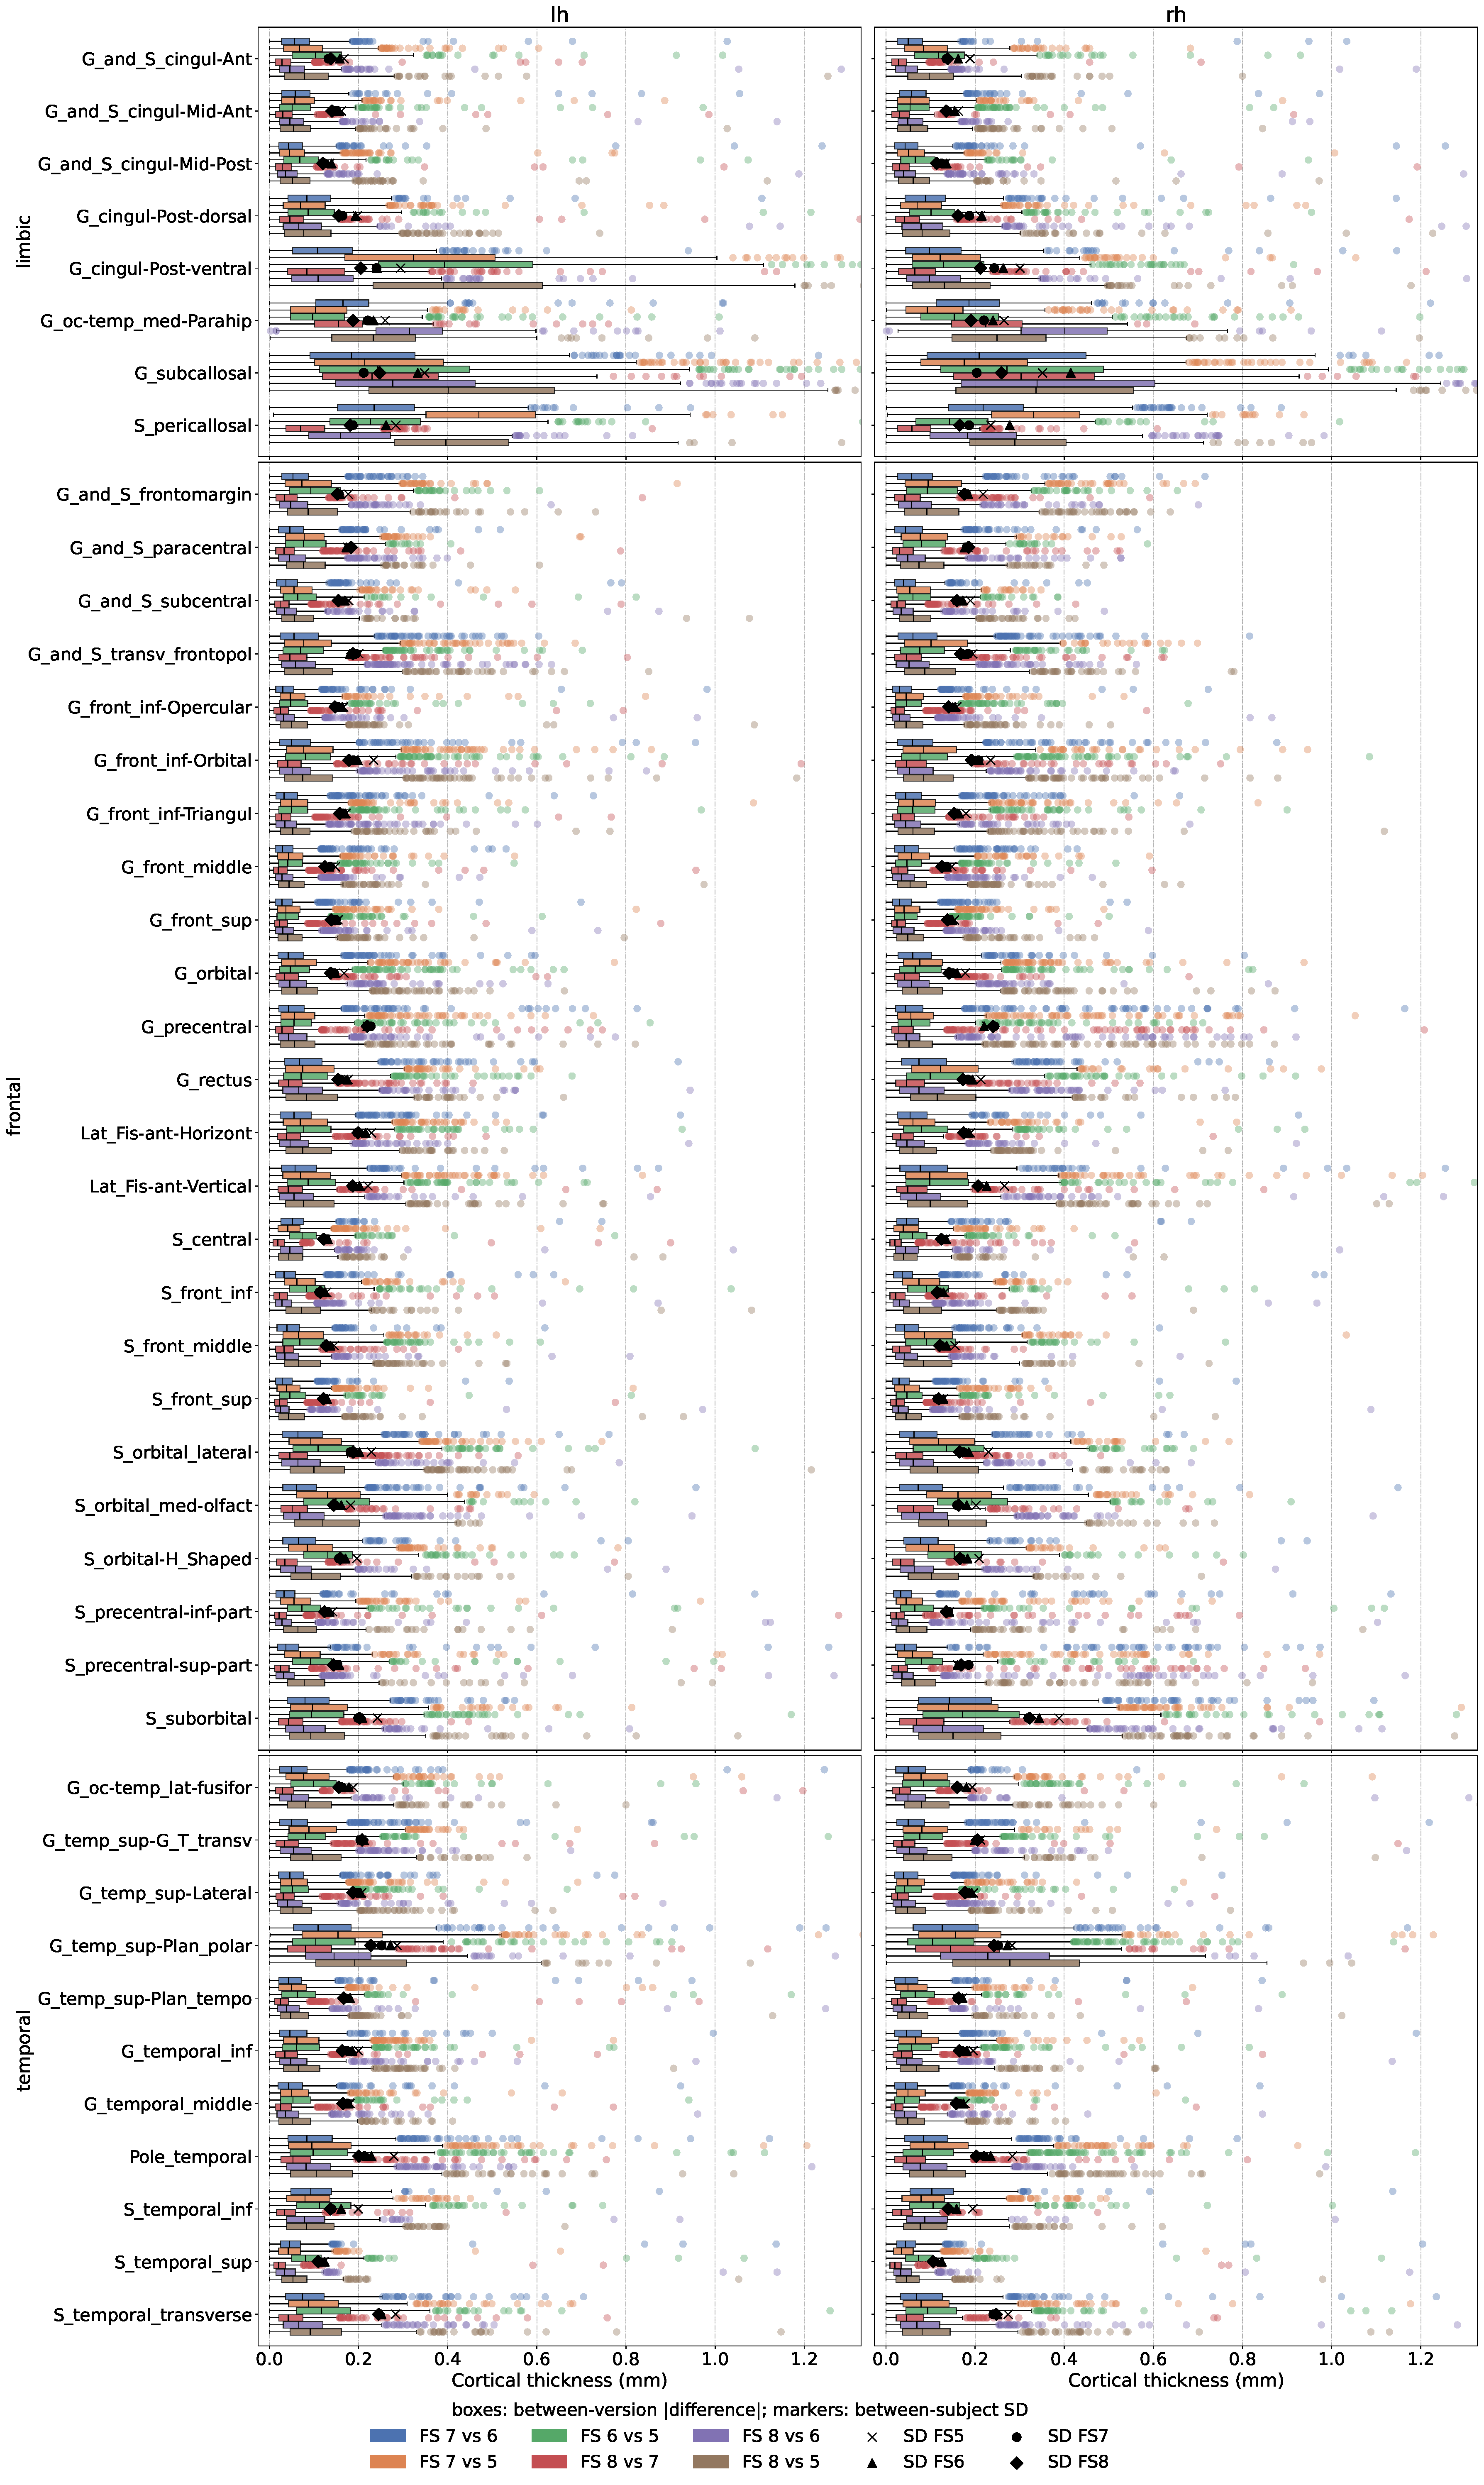
\includegraphics[width=\linewidth,height=0.8\textheight,keepaspectratio]{variability_ct_part1}
\caption{Between-version (\rev{n = 6 version pairs}) and between-subject (\rev{n = 830 images}) cortical thickness
variability \rev{in the left and right hemispheres, (a) limbic, frontal and temporal regions, (b) occipital,
parietal and other regions; outliers beyond the x-axis range are not shown}. Absolute difference between FreeSurfer versions represented as
box plots, standard deviations \rev{of each version} represented as black markers.}\label{fig:6}
\end{figure}

\begin{figure}[H]
\ContinuedFloat
\centering
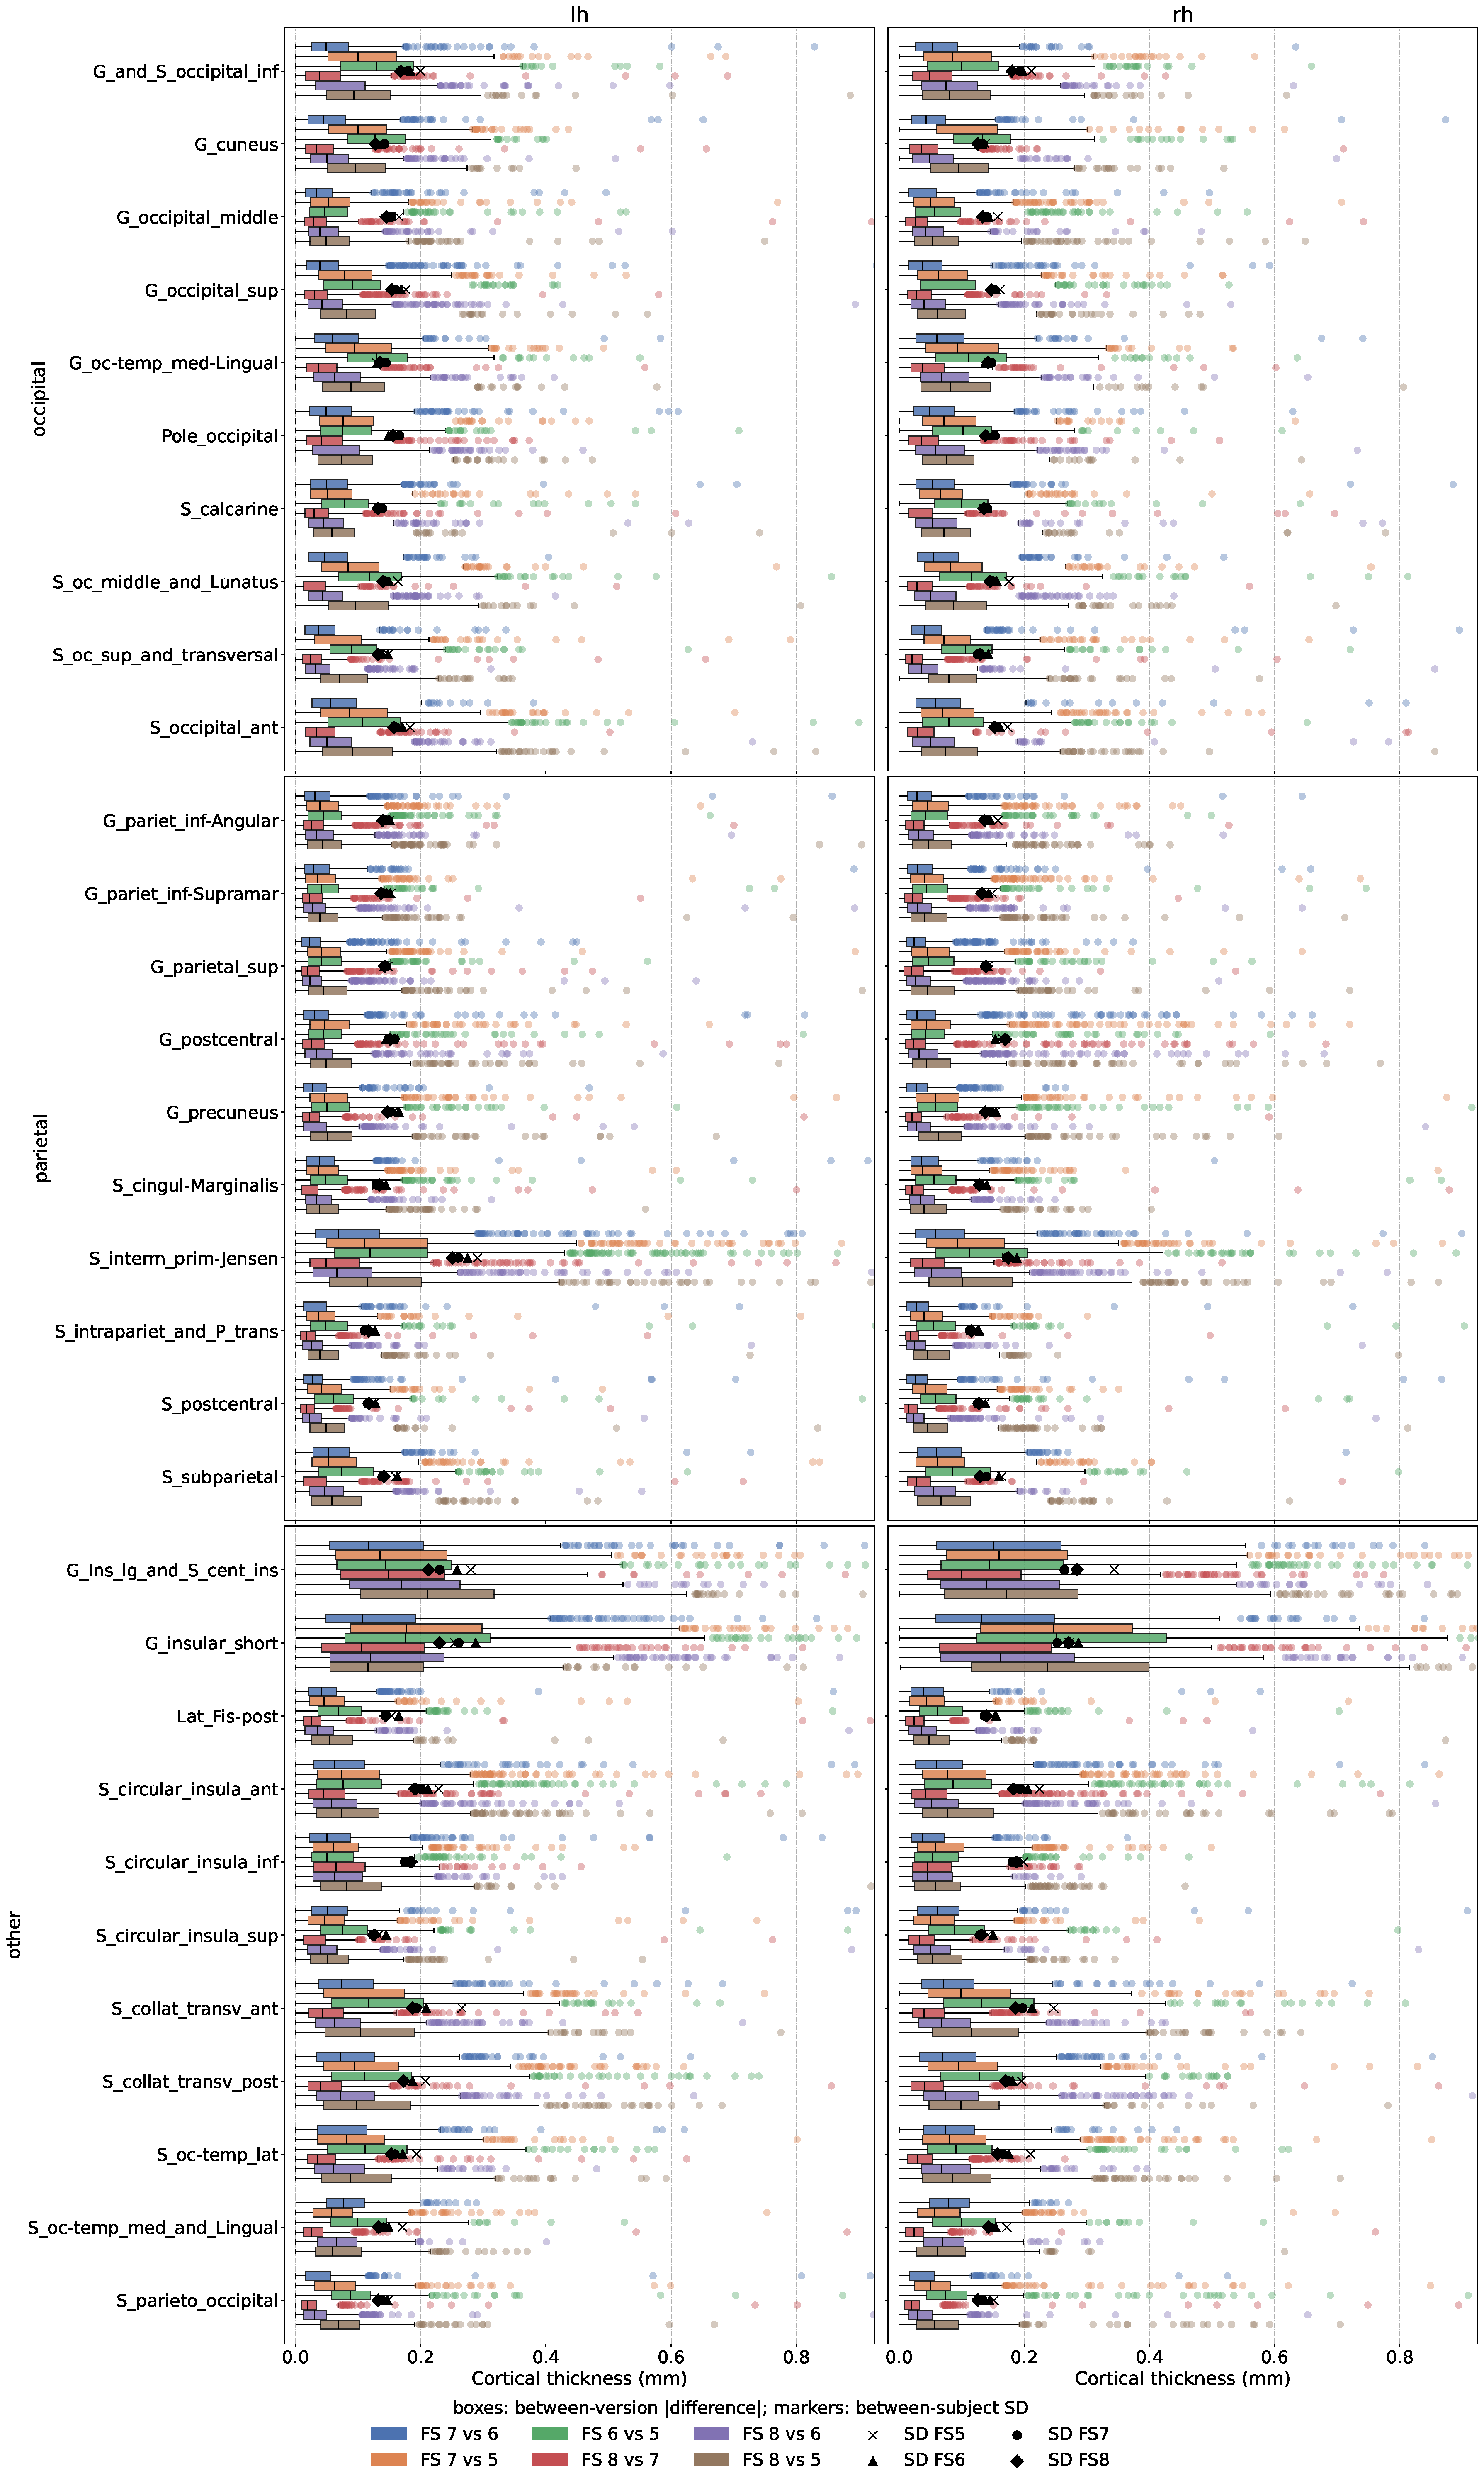
\includegraphics[width=\linewidth,height=0.8\textheight,keepaspectratio]{variability_ct_part2}
\caption{\rev{(continued) (b) Occipital, parietal and other regions.}}
\end{figure}

\rev{There were no group differences (HC vs PD) in FreeSurfer variability after correction for multiple
comparisons, except in one region: the left pericallosal sulcus thickness for FS8 vs FS6 ($t = -3.67$, $p < .001$;
1 of 2,898 tests). Adjusted for image quality and scanner manufacturer, this difference remained, and two other
tests became significant (thickness for FS6 vs FS5, volume for FS8 vs FS5; 3 of 2,898 tests). Results are
reported in Tables S4 and S5.}

\subsubsection*{Replication sample}

\rev{We tested differences between FreeSurfer versions in the estimation of the structural metrics in the PD
patients of the replication sample (201 images). As in the main sample, the versions differed in the majority of
the regions (Table S6, Figure~\ref{fig:1}). FS7 and FS6 differed in volume in 59\% of the regions (49\% of the
subcortical structures; 81\% in limbic, 67\% in frontal, 64\% in temporal, 40\% in occipital, 60\% in parietal
regions), in surface area in 76\% and in thickness in 76\%. FS7 and FS5 differed in volume in 76\% (92\% of the
subcortical structures), surface area in 71\% and thickness in 69\% (95\% in occipital regions). FS6 and FS5
differed in volume in 73\% (82\% subcortical), surface area in 70\% and thickness in 86\% (100\% in occipital and
parietal regions). The FS8 comparisons followed the main sample: FS8 and FS7 were the closest pair for surface area
(31\%) and thickness (45\%; 94\% in limbic but 15\% in parietal regions), but differed in 90\% of the subcortical
structures, while FS8 differed from FS6 and FS5 in 64--79\% of the regions for volume, 67--72\% for surface area
and 68--82\% for thickness.

The regions that differed between versions were largely the same in both samples: the Sørensen--Dice coefficient
between the sets of significant regions of PPMI and QPN was .83--.94 for volume, .89--.91 for surface area and
.83--.94 for thickness in the pairs of FS5--7 and FS8 vs FS5--6, and lowest for FS8 vs FS7 (.86, .69 and .72), the
pair with the fewest differences. Software variability in QPN PD differed from that in PPMI PD in 97 of the 2,898
tests (3\%), mostly for thickness (66 tests); in 84 of the 97, the differences between versions were smaller in
QPN. Within QPN, PD patients and the 69 healthy controls of the release did not differ in software variability (1
of 2,898 tests), as in PPMI.}

\subsection{Stage II: impact of measurement differences on the relationships between structural brain measurements and clinical outcomes}

\subsubsection*{Subcortical analyses}

We tested the group differences (PD vs HC) in subcortical volumes at baseline. To quantify the impact of
FreeSurfer versions on analysis outcomes, we calculated the \rev{Sørensen--Dice} coefficients between (1) the set
of regions with significant differences between PD and HC computed with FreeSurfer version A, and (2) the set of
regions with significant differences between PD and HC computed with FreeSurfer version B. \rev{At baseline, FS5
found four significant structures (left and right thalamus and hippocampus) and FS6 three (left and right
thalamus, right hippocampus), a Sørensen--Dice coefficient of .86. The coefficient was .86 between FS7 and FS6, .75
between FS7 and FS5, .67 between FS8 and FS6, and .57 between FS8 and FS7 and between FS8 and FS5. The bilateral thalamus was
significant in every version; FS7 additionally found the right pallidum, and FS8 the left accumbens area but not
the right hippocampus.} Results are reported in Table~\ref{tab:2}. \rev{In every version, the significant baseline differences were larger volumes in PD-non-MCI than in HC (sign of the age- and sex-adjusted group difference; 7 to 9 significant structures per version). This direction was unchanged with MRIQC total SNR and scanner manufacturer as covariates (Table S7) and with FreeSurfer's estimated total intracranial volume (eTIV) as a covariate, which reduced the differences by about a third (FS7: left thalamus 313 to 205 mm$^3$, brainstem 1043 to 709 mm$^3$) and the significant structures to 1 to 5 per version, all but one (right choroid plexus in FS6) larger in PD-non-MCI.}

We investigated group differences (PD vs HC) in the rate of change of subcortical volumes. \rev{Only one structure
was significant in FS5 (right caudate) and in FS8 (left caudate), and none in FS6 and FS7, so the} Sørensen--Dice
coefficients of the significant results across all FS versions were zero. Results are reported in
Table~\ref{tab:2}. Software variability has a substantial impact on both baseline and longitudinal analysis, even
though the lack of significance in the longitudinal analysis would deserve additional studies. \rev{With the
image-quality and scanner covariates, the significant structures were the same except in FS5 at baseline (bilateral
thalamus only) and in FS8 at baseline (right hippocampus added; Table S7).}

\begin{table}[H]
\centering\small
\caption{Group differences (\rev{PD-non-MCI vs HC}) in subcortical volumes at baseline and longitudinal group
differences in the rate of change in subcortical volumes.}\label{tab:2}
\begin{tabular}{lrrrrrrrr}
\toprule
 & \multicolumn{2}{c}{FS5} & \multicolumn{2}{c}{FS6} & \multicolumn{2}{c}{FS7} & \multicolumn{2}{c}{FS8} \\
\cmidrule(lr){2-3}\cmidrule(lr){4-5}\cmidrule(lr){6-7}\cmidrule(lr){8-9}
ROI & $F$ & $p$ & $F$ & $p$ & $F$ & $p$ & $F$ & $p$ \\
\midrule
\multicolumn{9}{l}{\textit{Baseline}} \\
Left-Thalamus & 10.940 & $\mathbf{0.0011}$ & 12.180 & $\mathbf{5.6{\times}10^{-4}}$ & 13.172 & $\mathbf{3.4{\times}10^{-4}}$ & 11.221 & $\mathbf{9.2{\times}10^{-4}}$ \\
Left-Caudate & 0.046 & $0.83$ & 0.004 & $0.95$ & 0.023 & $0.88$ & 0.006 & $0.94$ \\
Left-Putamen & 1.750 & $0.19$ & 3.401 & $0.066$ & 2.632 & $0.11$ & 1.424 & $0.23$ \\
Left-Pallidum & 3.003 & $0.084$ & 3.683 & $0.056$ & 7.467 & $0.0067$ & 1.315 & $0.25$ \\
Left-Hippocampus & 8.747 & $\mathbf{0.0034}$ & 7.391 & $0.0070$ & 6.685 & $0.010$ & 4.541 & $0.034$ \\
Left-Amygdala & 2.207 & $0.14$ & 2.972 & $0.086$ & 3.652 & $0.057$ & 3.889 & $0.050$ \\
Left-Accumbens-area & 8.235 & $0.0044$ & 3.774 & $0.053$ & 6.177 & $0.014$ & 11.954 & $\mathbf{6.3{\times}10^{-4}}$ \\
Right-Thalamus & 9.470 & $\mathbf{0.0023}$ & 11.840 & $\mathbf{6.7{\times}10^{-4}}$ & 15.583 & $\mathbf{1.0{\times}10^{-4}}$ & 9.824 & $\mathbf{0.0019}$ \\
Right-Caudate & 0.013 & $0.91$ & 0.071 & $0.79$ & 0.123 & $0.73$ & 0.037 & $0.85$ \\
Right-Putamen & 1.020 & $0.31$ & 1.282 & $0.26$ & 1.878 & $0.17$ & 1.284 & $0.26$ \\
Right-Pallidum & 3.771 & $0.053$ & 7.760 & $0.0057$ & 16.162 & $\mathbf{7.5{\times}10^{-5}}$ & 3.431 & $0.065$ \\
Right-Hippocampus & 11.633 & $\mathbf{7.5{\times}10^{-4}}$ & 13.880 & $\mathbf{2.4{\times}10^{-4}}$ & 14.412 & $\mathbf{1.8{\times}10^{-4}}$ & 7.642 & $0.0061$ \\
Right-Amygdala & 1.103 & $0.29$ & 5.816 & $0.017$ & 7.747 & $0.0058$ & 6.113 & $0.014$ \\
Right-Accumbens-area & 4.422 & $0.036$ & 6.470 & $0.012$ & 8.178 & $0.0046$ & 8.276 & $0.0043$ \\
\midrule
\multicolumn{9}{l}{\textit{Longitudinal}} \\
Left-Thalamus & 0.747 & $0.39$ & 0.000 & $0.99$ & 0.196 & $0.66$ & 0.115 & $0.74$ \\
Left-Caudate & 4.078 & $0.044$ & 1.644 & $0.20$ & 2.012 & $0.16$ & 14.440 & $\mathbf{1.8{\times}10^{-4}}$ \\
Left-Putamen & 0.803 & $0.37$ & 2.126 & $0.15$ & 0.270 & $0.60$ & 0.955 & $0.33$ \\
Left-Pallidum & 0.000 & $0.99$ & 4.950 & $0.027$ & 5.095 & $0.025$ & 0.030 & $0.86$ \\
Left-Hippocampus & 0.243 & $0.62$ & 0.944 & $0.33$ & 0.210 & $0.65$ & 2.415 & $0.12$ \\
Left-Amygdala & 0.666 & $0.41$ & 0.229 & $0.63$ & 0.048 & $0.83$ & 0.278 & $0.60$ \\
Left-Accumbens-area & 0.001 & $0.98$ & 1.288 & $0.26$ & 0.430 & $0.51$ & 0.739 & $0.39$ \\
Right-Thalamus & 0.359 & $0.55$ & 0.186 & $0.67$ & 0.004 & $0.95$ & 3.687 & $0.056$ \\
Right-Caudate & 14.632 & $\mathbf{1.6{\times}10^{-4}}$ & 4.003 & $0.046$ & 1.588 & $0.21$ & 6.776 & $0.0097$ \\
Right-Putamen & 1.795 & $0.18$ & 0.695 & $0.41$ & 1.083 & $0.30$ & 3.741 & $0.054$ \\
Right-Pallidum & 0.005 & $0.95$ & 1.957 & $0.16$ & 0.026 & $0.87$ & 5.191 & $0.023$ \\
Right-Hippocampus & 3.979 & $0.047$ & 1.067 & $0.30$ & 0.036 & $0.85$ & 3.360 & $0.068$ \\
Right-Amygdala & 0.675 & $0.41$ & 0.204 & $0.65$ & 0.294 & $0.59$ & 0.083 & $0.77$ \\
Right-Accumbens-area & 0.511 & $0.48$ & 1.693 & $0.19$ & 3.952 & $0.048$ & 1.977 & $0.16$ \\
\bottomrule
\end{tabular}

\par\smallskip\parbox{\linewidth}{\footnotesize \rev{ANCOVA (age and sex; longitudinal: also time between the
visits) was used to test differences between PD-non-MCI (n = 138) and HC (n = 137). Raw p-values, exact; in bold:
significant after Bonferroni correction ($p < 0.05/14 = 0.0036$).}}
\end{table}

We investigated correlation between UPDRS score and subcortical volumes at baseline. \rev{The correlation between
the right putamen volume and the UPDRS score was significant after Bonferroni correction in FS6 only ($r = -.25$,
$p = .003$); it was close to the threshold in FS7 ($r = -.25$, $p = .004$) and FS5 ($r = -.22$, $p = .010$) and
weaker in FS8 ($r = -.20$, $p = .017$).} Results are reported in Table~\ref{tab:3}.

We investigated correlation between the change in UPDRS score and the rate of change of subcortical volumes. No
result remained significant after Bonferroni correction. Results are reported in Table~\ref{tab:3}. \rev{With the
image-quality and scanner covariates, the baseline right putamen correlation was no longer significant in FS6, and
the longitudinal correlation with the right caudate became significant in FS6 (Table S7).}

\begin{table}[H]
\centering\small
\caption{Correlation between the UPDRS score and subcortical volumes at baseline, and longitudinal correlation
between the change in UPDRS score and the rate of change in subcortical volumes.}\label{tab:3}
\begin{tabular}{lrrrrrrrr}
\toprule
 & \multicolumn{2}{c}{FS5} & \multicolumn{2}{c}{FS6} & \multicolumn{2}{c}{FS7} & \multicolumn{2}{c}{FS8} \\
\cmidrule(lr){2-3}\cmidrule(lr){4-5}\cmidrule(lr){6-7}\cmidrule(lr){8-9}
ROI & $r$ & $p$ & $r$ & $p$ & $r$ & $p$ & $r$ & $p$ \\
\midrule
\multicolumn{9}{l}{\textit{Baseline}} \\
Left-Thalamus & 0.010 & $0.91$ & -0.023 & $0.79$ & -0.018 & $0.83$ & -0.038 & $0.66$ \\
Left-Caudate & -0.220 & $0.010$ & -0.192 & $0.025$ & -0.197 & $0.022$ & -0.141 & $0.10$ \\
Left-Putamen & -0.185 & $0.031$ & -0.198 & $0.021$ & -0.218 & $0.011$ & -0.225 & $0.0085$ \\
Left-Pallidum & -0.189 & $0.027$ & -0.073 & $0.40$ & -0.144 & $0.095$ & -0.071 & $0.41$ \\
Left-Hippocampus & -0.125 & $0.15$ & -0.108 & $0.21$ & -0.125 & $0.15$ & -0.116 & $0.18$ \\
Left-Amygdala & -0.061 & $0.48$ & -0.105 & $0.22$ & -0.114 & $0.19$ & -0.248 & $0.0037$ \\
Left-Accumbens-area & 0.111 & $0.20$ & 0.070 & $0.42$ & 0.077 & $0.38$ & -0.042 & $0.63$ \\
Right-Thalamus & 0.010 & $0.91$ & -0.014 & $0.88$ & -0.046 & $0.59$ & -0.089 & $0.30$ \\
Right-Caudate & -0.133 & $0.12$ & -0.132 & $0.13$ & -0.138 & $0.11$ & -0.127 & $0.14$ \\
Right-Putamen & -0.221 & $0.0097$ & -0.254 & $\mathbf{0.0029}$ & -0.248 & $0.0036$ & -0.204 & $0.017$ \\
Right-Pallidum & -0.006 & $0.94$ & 0.047 & $0.58$ & 0.009 & $0.91$ & 0.012 & $0.89$ \\
Right-Hippocampus & -0.215 & $0.012$ & -0.170 & $0.048$ & -0.200 & $0.020$ & -0.171 & $0.047$ \\
Right-Amygdala & -0.125 & $0.15$ & -0.125 & $0.15$ & -0.201 & $0.019$ & -0.244 & $0.0043$ \\
Right-Accumbens-area & -0.010 & $0.91$ & 0.018 & $0.84$ & -0.046 & $0.59$ & -0.052 & $0.55$ \\
\midrule
\multicolumn{9}{l}{\textit{Longitudinal}} \\
Left-Thalamus & 0.115 & $0.19$ & 0.017 & $0.84$ & 0.026 & $0.77$ & -0.100 & $0.25$ \\
Left-Caudate & 0.036 & $0.68$ & -0.084 & $0.33$ & -0.021 & $0.81$ & -0.159 & $0.065$ \\
Left-Putamen & -0.049 & $0.58$ & 0.003 & $0.97$ & -0.068 & $0.43$ & -0.128 & $0.14$ \\
Left-Pallidum & 0.019 & $0.82$ & 0.122 & $0.16$ & 0.006 & $0.95$ & 0.090 & $0.30$ \\
Left-Hippocampus & 0.088 & $0.31$ & 0.055 & $0.52$ & 0.052 & $0.55$ & -0.049 & $0.57$ \\
Left-Amygdala & 0.103 & $0.23$ & -0.073 & $0.40$ & -0.003 & $0.97$ & -0.053 & $0.54$ \\
Left-Accumbens-area & -0.055 & $0.52$ & 0.061 & $0.48$ & 0.078 & $0.37$ & 0.071 & $0.42$ \\
Right-Thalamus & -0.001 & $0.99$ & -0.009 & $0.92$ & 0.016 & $0.85$ & 0.004 & $0.96$ \\
Right-Caudate & -0.107 & $0.21$ & -0.240 & $0.0050$ & -0.187 & $0.030$ & -0.102 & $0.24$ \\
Right-Putamen & 0.058 & $0.50$ & 0.175 & $0.043$ & 0.168 & $0.051$ & 0.087 & $0.32$ \\
Right-Pallidum & -0.030 & $0.73$ & -0.082 & $0.35$ & 0.028 & $0.74$ & 0.109 & $0.21$ \\
Right-Hippocampus & 0.147 & $0.090$ & 0.017 & $0.85$ & 0.029 & $0.74$ & -0.103 & $0.24$ \\
Right-Amygdala & 0.025 & $0.77$ & -0.047 & $0.59$ & -0.151 & $0.080$ & -0.006 & $0.94$ \\
Right-Accumbens-area & -0.104 & $0.23$ & 0.009 & $0.91$ & -0.005 & $0.95$ & 0.093 & $0.28$ \\
\bottomrule
\end{tabular}

\par\smallskip\parbox{\linewidth}{\footnotesize Partial correlation \rev{(age and sex; longitudinal: also time
between the visits) in PD-non-MCI patients (n = 138)} was used to test the correlations. \rev{Raw p-values, exact;
in bold: significant after Bonferroni correction ($p < 0.05/14 = 0.0036$).}}
\end{table}

\rev{Figures~\ref{fig:subgroup} and~\ref{fig:subcorr} show the results of Tables~\ref{tab:2} and~\ref{tab:3} in the
brain, with the colour scale of the vertex-wise maps.}

\begin{figure}[H]
\centering
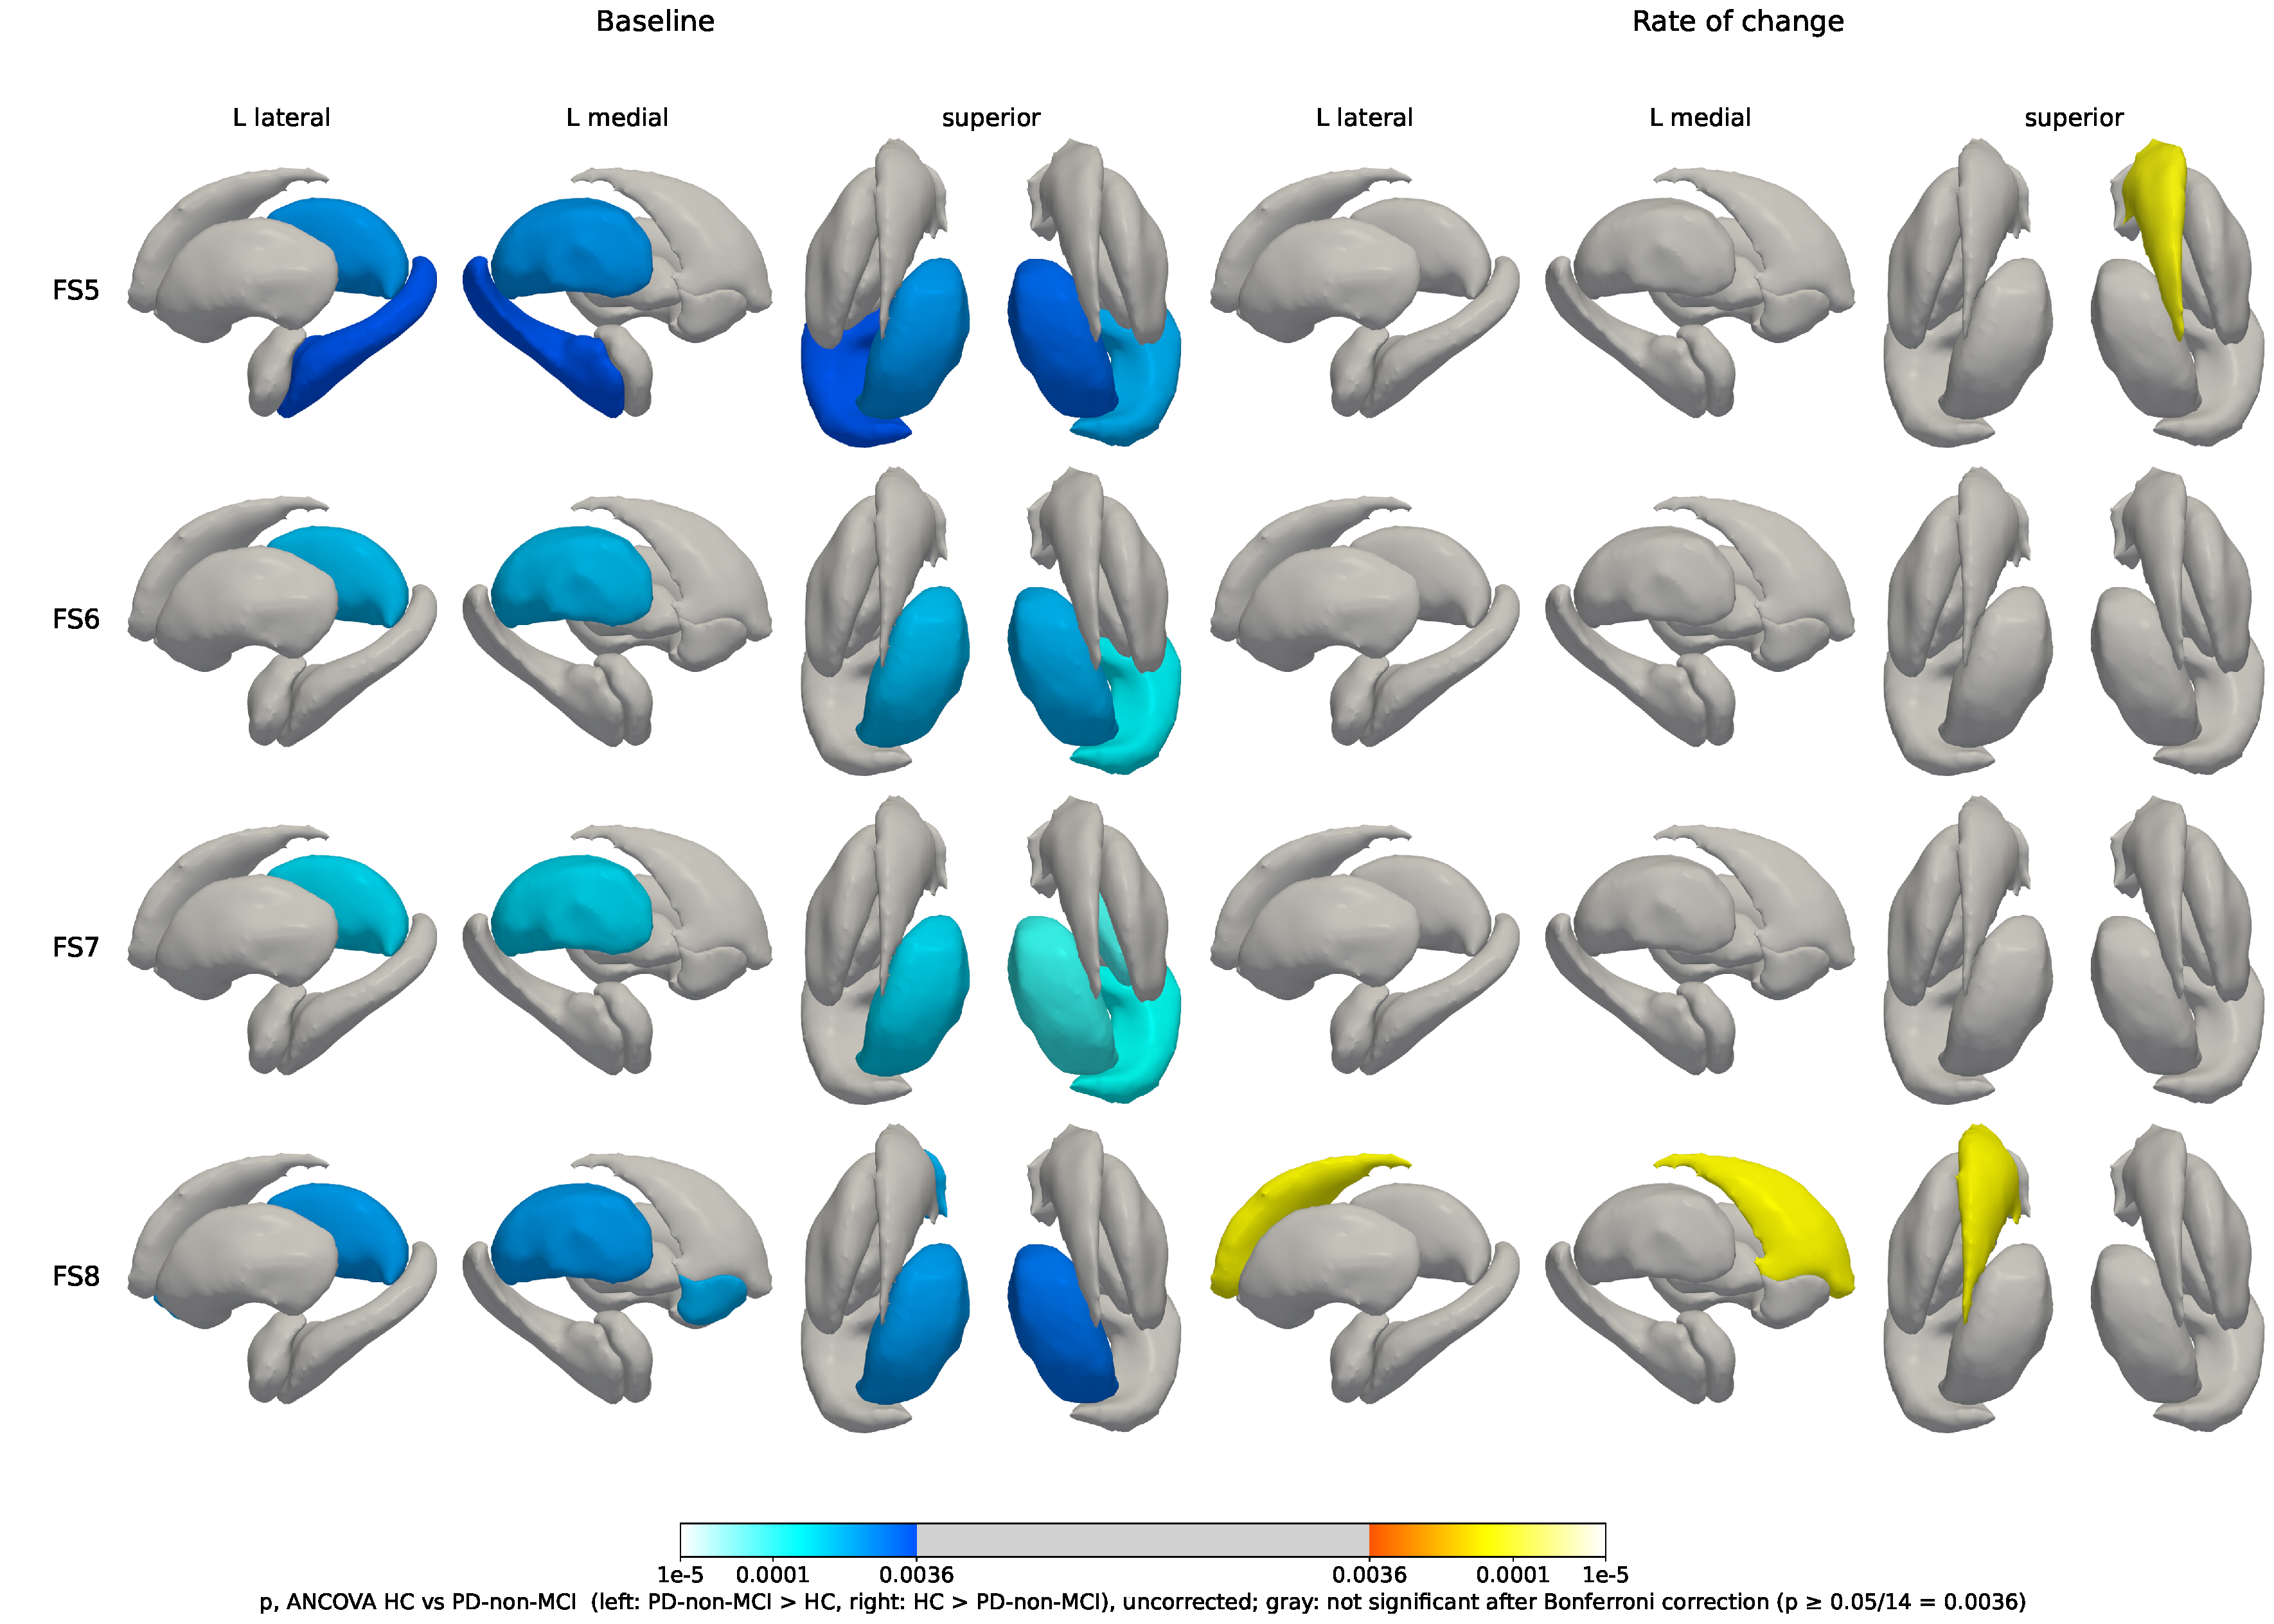
\includegraphics[width=\linewidth]{fig_subcortical_group}
\caption{\rev{Group differences (HC vs PD-non-MCI) in subcortical volumes at baseline and in their rate of change
(ANCOVA, Table~\ref{tab:2}), one row per FreeSurfer version, on the subcortical structures of fsaverage. Colour: p-value of each structure, signed by the direction of the age- and sex-adjusted group difference (red: larger in HC; blue: larger in PD-non-MCI); coloured: significant after Bonferroni correction (uncorrected $p < 0.05/14 = 0.0036$, the entries in bold in Table~\ref{tab:2}); gray: not significant after correction.}}\label{fig:subgroup}
\end{figure}

\begin{figure}[H]
\centering
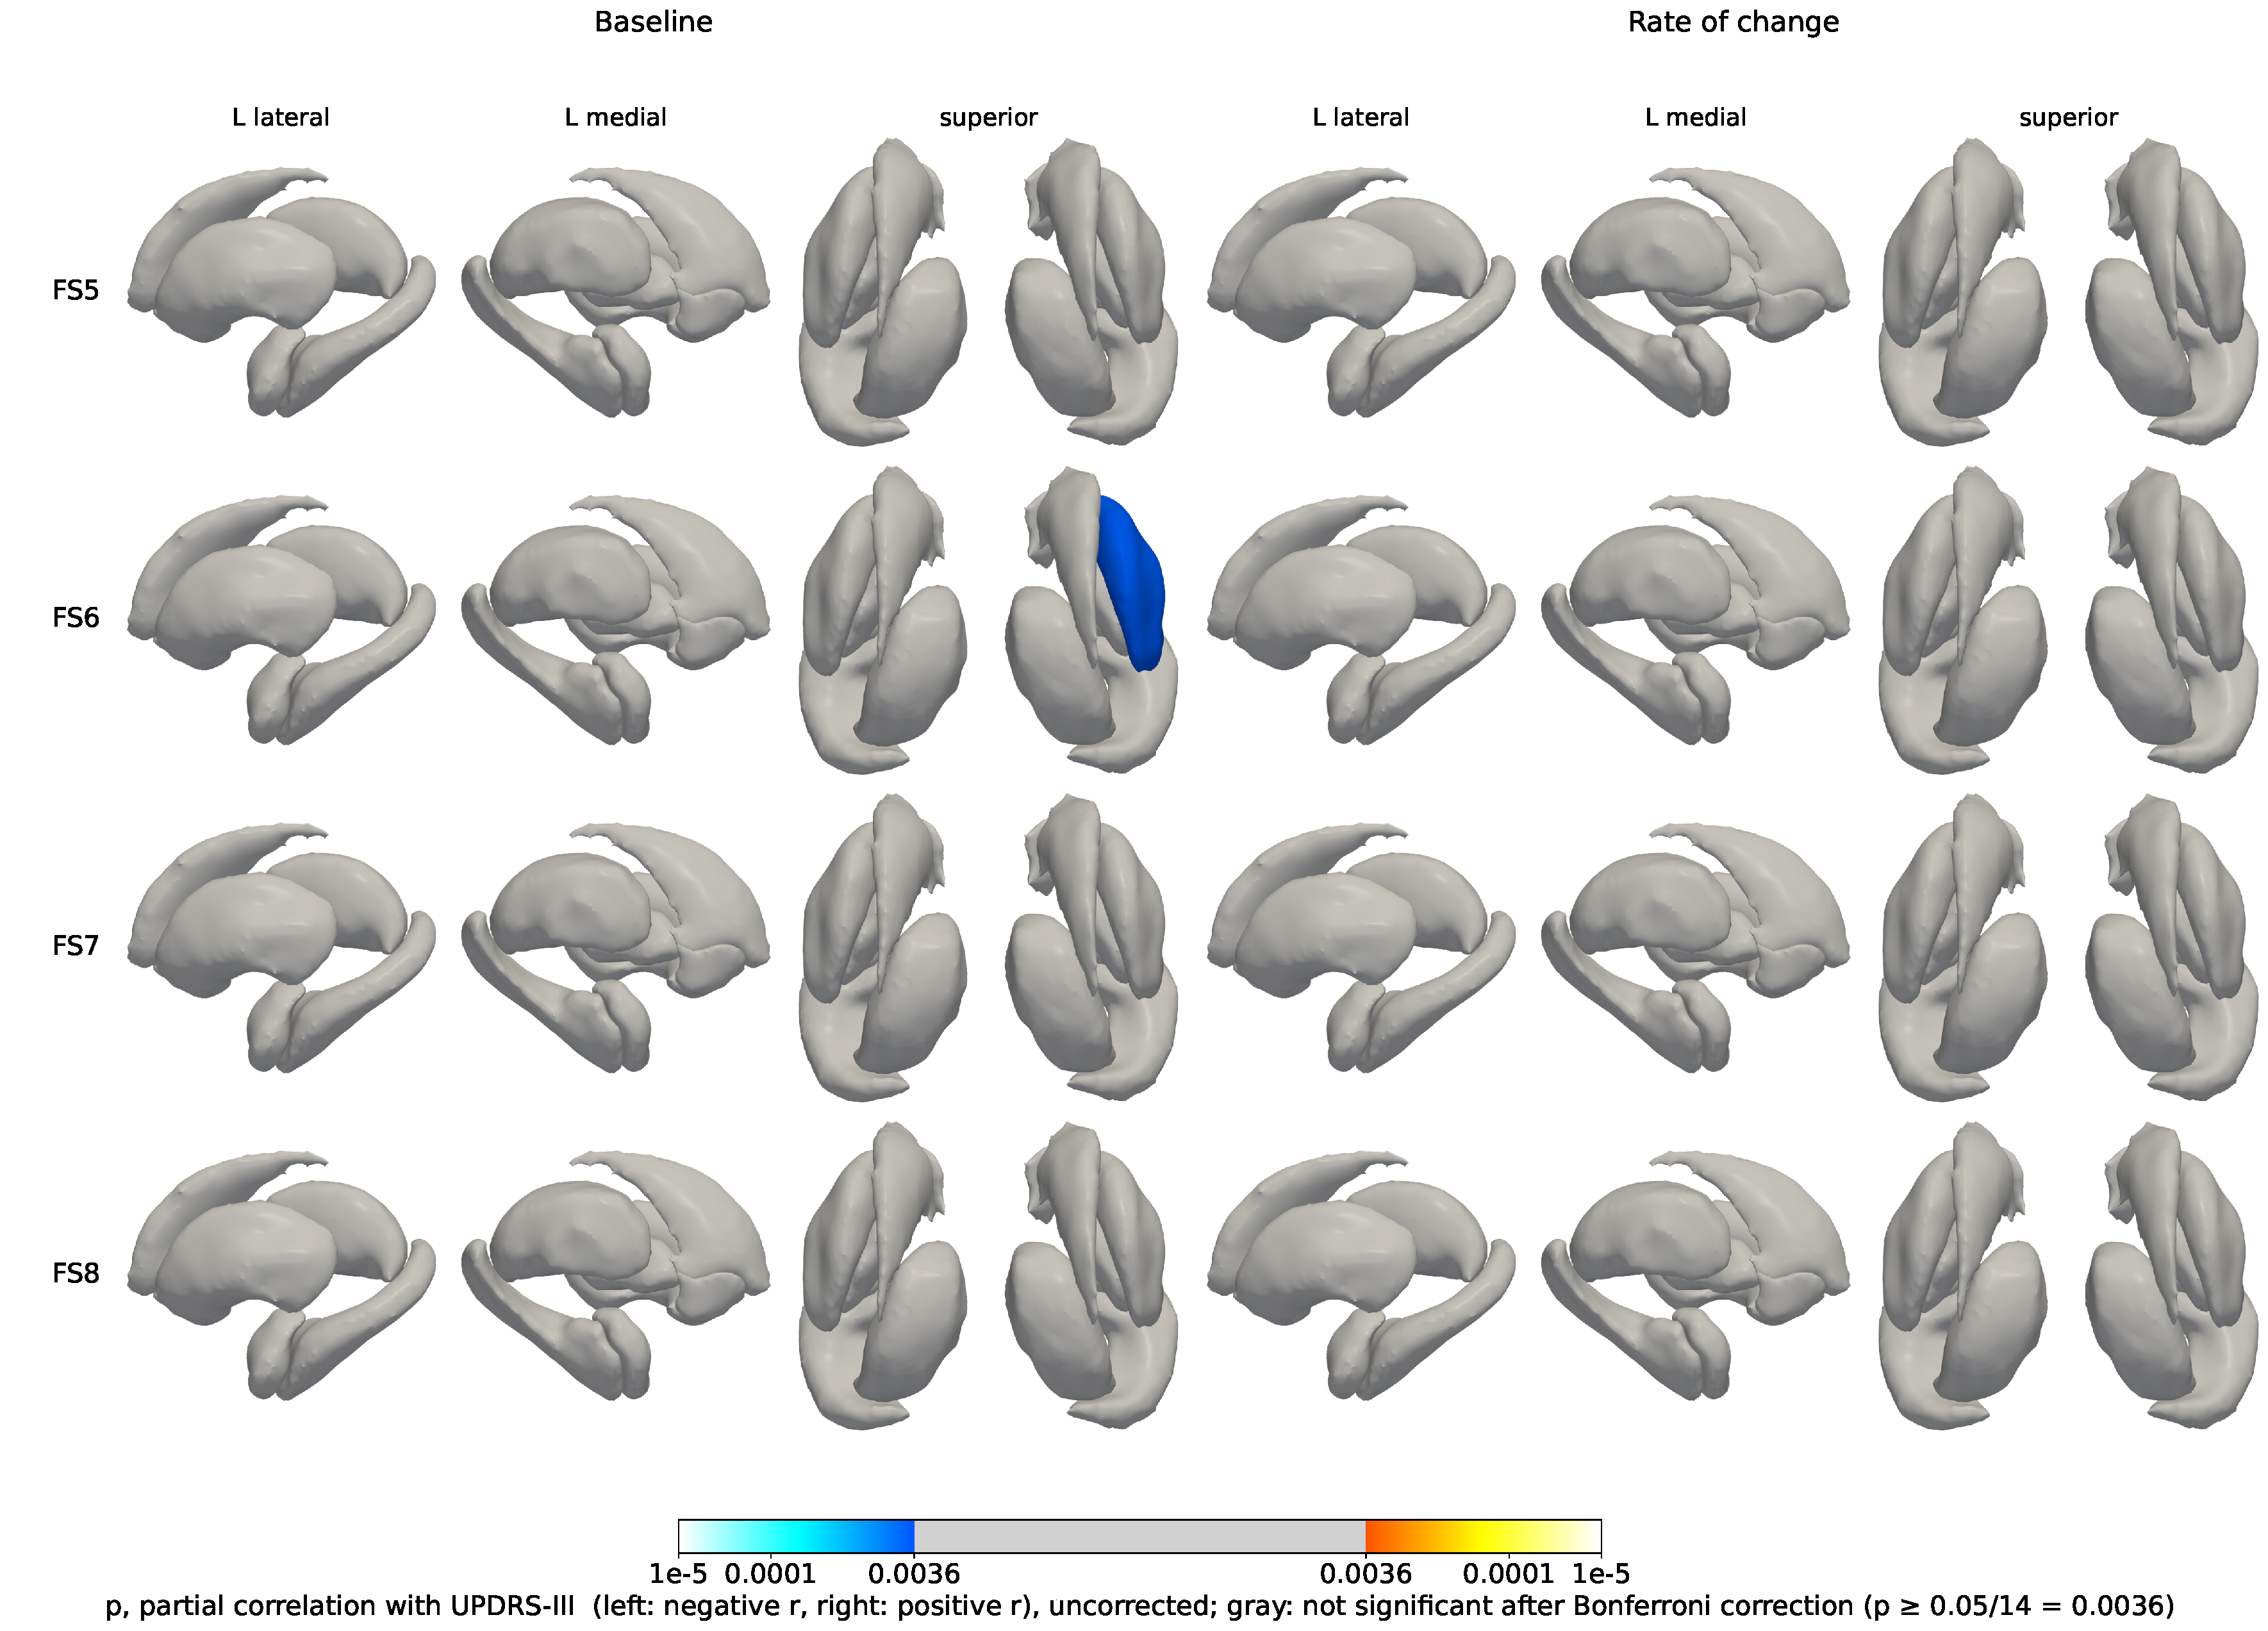
\includegraphics[width=\linewidth]{fig_subcortical_corr}
\caption{\rev{Partial correlation between UPDRS-III and subcortical volumes at baseline, and between the change in
UPDRS-III and the rate of change in volume (Table~\ref{tab:3}), one row per FreeSurfer version. Colour: p-value of each structure, signed by the correlation (red: positive; blue: negative); coloured: significant after Bonferroni correction (uncorrected $p < 0.05/14 = 0.0036$, the entries in bold in Table~\ref{tab:3}); gray: not significant after correction.}}\label{fig:subcorr}
\end{figure}

\subsubsection*{Vertex-wise analyses}

\paragraph{Correlation analyses}
We found significant vertex-wise correlations between UPDRS score and cortical thickness at baseline. More
significant clusters were found in FS5 \rev{(8 clusters) than in FS6 (3), FS7 (2), and FS8 (2). The left
precentral or postcentral gyrus was found in every version.} In the longitudinal analysis the rate of change in
cortical thickness \rev{significantly correlated with the rate of change in UPDRS score in one region in FS6 (left
lingual gyrus) and two in FS8 (right precuneus and middle temporal gyrus), and in none in FS5 and FS7.} The results
are reported in Table~\ref{tab:4}.

\begin{table}[H]
\centering\small
\caption{Vertex-wise correlation between UPDRS score and cortical thickness at baseline, and the correlation
between the rate of change in UPDRS and the rate of change in cortical thickness.}\label{tab:4}
\begin{tabular}{llrrrrr}
\toprule
Version & Region & Size (mm$^2$) & MNI X & MNI Y & MNI Z & Max \\
\midrule
\multicolumn{7}{l}{\textit{Baseline}} \\
\cmidrule(lr){1-7}
FS5 & L precentral & 1745.65 & -43.5 & -12.7 & 42.8 & -5.56 \\
 & L postcentral & 1231.95 & -35.4 & -34.5 & 60.0 & -4.25 \\
 & L parsopercularis & 934.71 & -41.7 & 12.0 & 22.8 & -3.74 \\
 & L inferiorparietal & 1016.22 & -29.3 & -66.3 & 28.3 & -3.32 \\
 & R precentral & 1630.09 & 23.5 & -26.0 & 50.3 & -4.99 \\
 & R lateraloccipital & 993.25 & 47.4 & -78.1 & 7.4 & -4.21 \\
 & R lateralorbitofrontal & 982.76 & 38.7 & 27.9 & -16.0 & -3.49 \\
 & R lateraloccipital & 1096.74 & 29.6 & -86.7 & -12.9 & -3.03 \\
\rowcolor{gray!12}FS6 & L lingual & 1393.97 & -7.1 & -93.0 & -6.8 & -3.29 \\
\rowcolor{gray!12} & L postcentral & 1283.27 & -35.4 & -33.9 & 63.9 & -4.73 \\
\rowcolor{gray!12} & R pericalcarine & 2272.15 & 16.1 & -97.7 & 1.4 & -4.80 \\
FS7 & L precentral & 1080.27 & -46.4 & -11.3 & 46.1 & -3.50 \\
 & R insula & 975.92 & 33.5 & 18.9 & 1.0 & -2.70 \\
\rowcolor{gray!12}FS8 & L postcentral & 1014.60 & -36.5 & -34.1 & 61.2 & -4.84 \\
\rowcolor{gray!12} & R lateraloccipital & 1391.04 & 25.0 & -94.8 & -13.4 & -4.03 \\
\multicolumn{7}{l}{\textit{Longitudinal}} \\
\cmidrule(lr){1-7}
FS5 & \multicolumn{6}{l}{no significant cluster} \\
\rowcolor{gray!12}FS6 & L lingual & 542.02 & -10.1 & -76.0 & -7.0 & -4.45 \\
FS7 & \multicolumn{6}{l}{no significant cluster} \\
\rowcolor{gray!12}FS8 & R precuneus & 939.78 & 7.7 & -37.2 & 37.9 & -3.85 \\
\rowcolor{gray!12} & R middletemporal & 729.51 & 49.5 & -31.9 & -8.8 & -3.91 \\
\bottomrule
\end{tabular}

\par\smallskip\parbox{\linewidth}{\footnotesize L, left; Max, maximum \rev{signed} $-\log_{10}$(p-value) in the
cluster; R, right. \rev{Regions: Desikan-Killiany label of the cluster's peak.} Partial correlation was used to
test the correlations \rev{(PD-non-MCI, n = 138)}. Cluster-wise p-value threshold was used at the p $<$ .05
level.}
\end{table}

\begin{figure}[H]
\centering
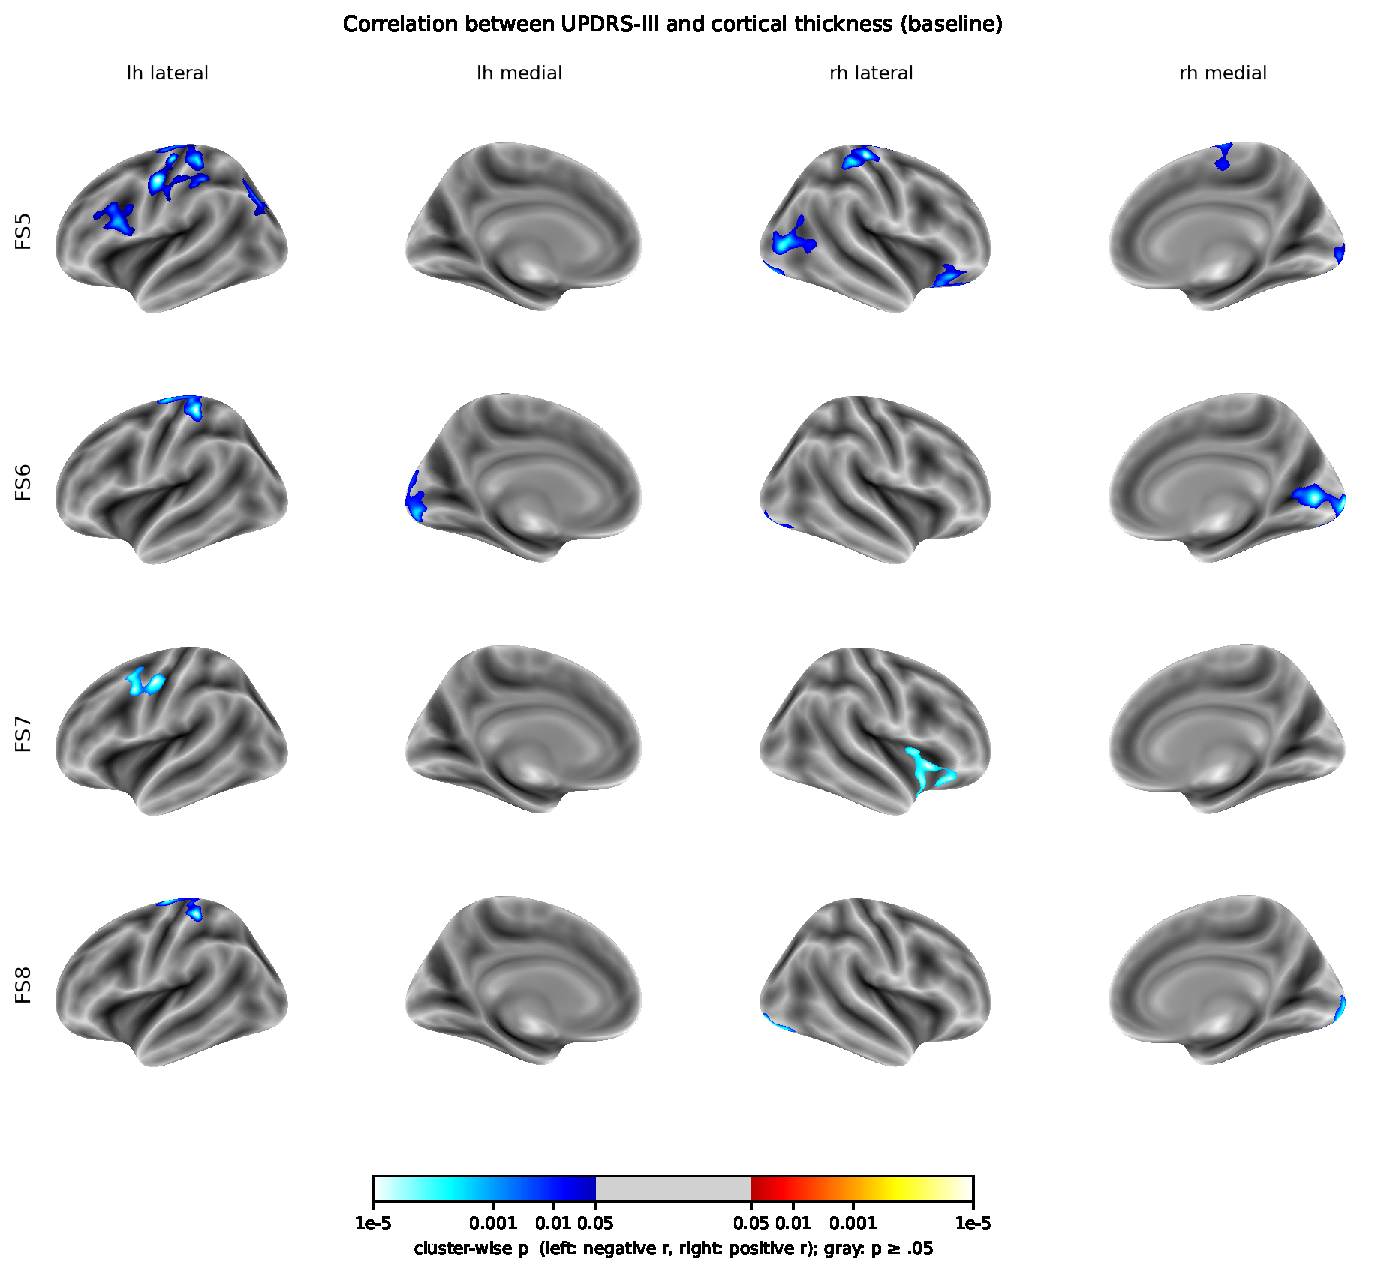
\includegraphics[width=\linewidth]{fig7_corr_base}
\caption{Vertex-wise correlation between UPDRS score and cortical thickness at baseline. \rev{Significant clusters
(cluster-wise p $<$ .05), signed $-\log_{10}$(p) on the fsaverage inflated surface.}}\label{fig:7}
\end{figure}

\begin{figure}[H]
\centering
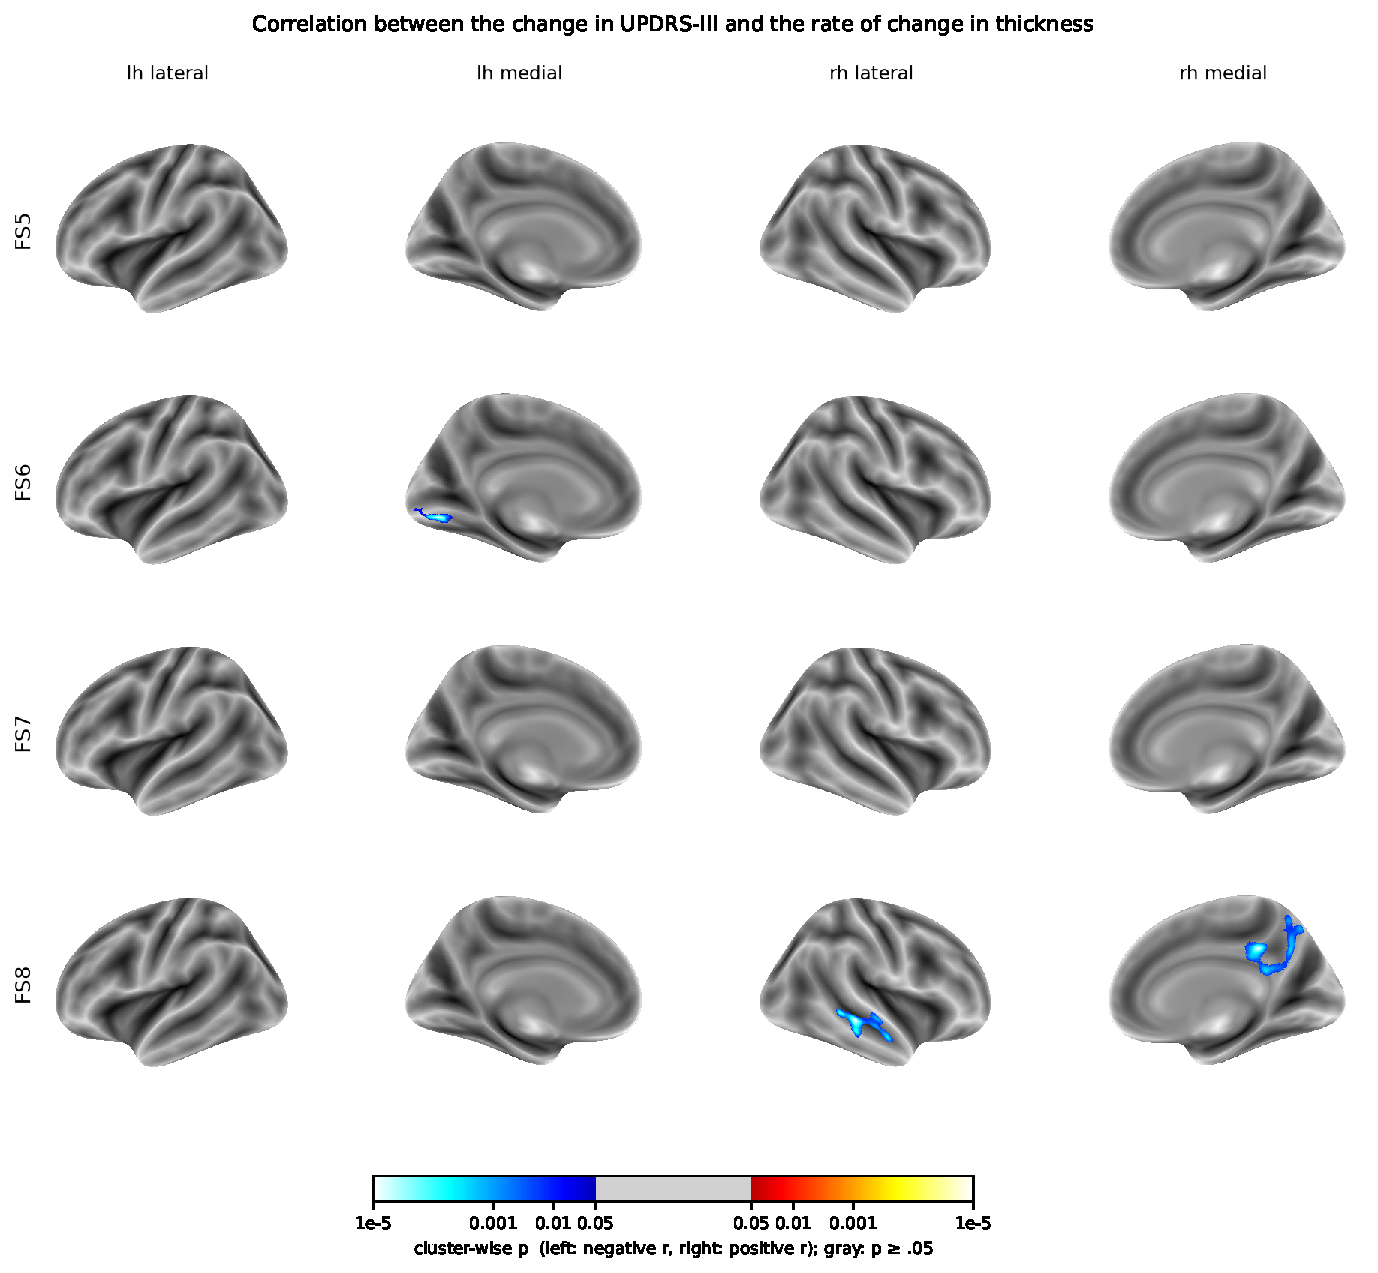
\includegraphics[width=\linewidth]{fig8_corr_long}
\caption{Vertex-wise correlation between the rate of change in UPDRS and the rate of change in cortical thickness.
Correlations in FreeSurfer 5 and 7 were not significant.}\label{fig:8}
\end{figure}

\paragraph{Group analyses}
\rev{There were significant vertex-wise group differences between HC and PD-non-MCI patients in cortical thickness
at baseline in two regions in FS5 (left postcentral and rostral middle frontal) and two in FS6 (right inferior
parietal and rostral middle frontal), and none in FS7 and FS8.} Additionally, we found significant group
differences in the rate of change in cortical \rev{thickness} in multiple regions across different FS versions.
More significant clusters were found in FS5 \rev{(7 clusters) than in FS6 (4), FS8 (2), and FS7 (1); the left
superior temporal gyrus was found in all four versions.} The results are reported in Table~\ref{tab:5}. \rev{With
the image-quality and scanner covariates, most longitudinal group differences disappeared (Table S8).}

\begin{table}[H]
\centering\small
\caption{Group differences (HC vs PD-non-MCI) in cortical thickness at baseline and in the rate of change in
cortical thickness.}\label{tab:5}
\begin{tabular}{llrrrrr}
\toprule
Version & Region & Size (mm$^2$) & MNI X & MNI Y & MNI Z & Max \\
\midrule
\multicolumn{7}{l}{\textit{Baseline}} \\
FS5 & L postcentral & 1073.97 & -49.6 & -17.7 & 35.8 & -3.61 \\
 & L rostralmiddlefrontal & 1252.90 & -40.1 & 28.5 & 20.0 & -3.28 \\
FS6 & R inferiorparietal & 1002.10 & 41.8 & -75.8 & 14.4 & -3.62 \\
 & R rostralmiddlefrontal & 996.83 & 40.8 & 31.0 & 19.2 & -2.63 \\
FS7 & \multicolumn{6}{l}{no significant cluster} \\
FS8 & \multicolumn{6}{l}{no significant cluster} \\
\multicolumn{7}{l}{\textit{Longitudinal}} \\
FS5 & L fusiform & 553.99 & -29.0 & -75.5 & -10.8 & -3.52 \\
 & L temporalpole & 915.32 & -39.3 & 12.1 & -36.6 & -3.19 \\
 & L inferiorparietal & 529.65 & -41.9 & -78.6 & 20.6 & -2.94 \\
 & L precentral & 544.73 & -16.5 & -19.1 & 67.2 & -2.90 \\
 & L superiortemporal & 561.68 & -61.5 & -29.1 & 6.4 & -2.66 \\
 & R caudalmiddlefrontal & 1614.73 & 25.5 & 3.8 & 46.9 & -4.98 \\
 & R supramarginal & 1091.20 & 58.2 & -26.6 & 40.0 & -2.96 \\
FS6 & L supramarginal & 857.10 & -61.2 & -31.4 & 34.5 & -2.24 \\
 & L superiortemporal & 804.85 & -61.7 & -29.7 & 0.7 & -3.07 \\
 & L lateraloccipital & 610.43 & -47.3 & -76.5 & 10.8 & -3.86 \\
 & L postcentral & 528.59 & -54.1 & -22.2 & 42.4 & -3.73 \\
FS7 & L superiortemporal & 694.51 & -46.0 & -5.9 & -16.9 & -2.87 \\
FS8 & L superiortemporal & 1070.52 & -47.7 & -13.4 & -8.6 & -3.59 \\
 & R fusiform & 692.99 & 32.7 & -72.8 & -12.7 & -2.40 \\
\bottomrule
\end{tabular}

\par\smallskip\parbox{\linewidth}{\footnotesize HC, healthy controls; L, left; Max, maximum \rev{signed}
$-\log_{10}$(p-value) in the cluster; MCI, mild cognitive impairment; PD, Parkinson's disease; R, right.
\rev{Regions: Desikan-Killiany label of the cluster's peak. General linear model with age and sex (longitudinal:
also time between the visits), HC n = 137, PD-non-MCI n = 138.} Cluster-wise p-value threshold was used at the
p $<$ .05 level.}
\end{table}

\begin{figure}[H]
\centering
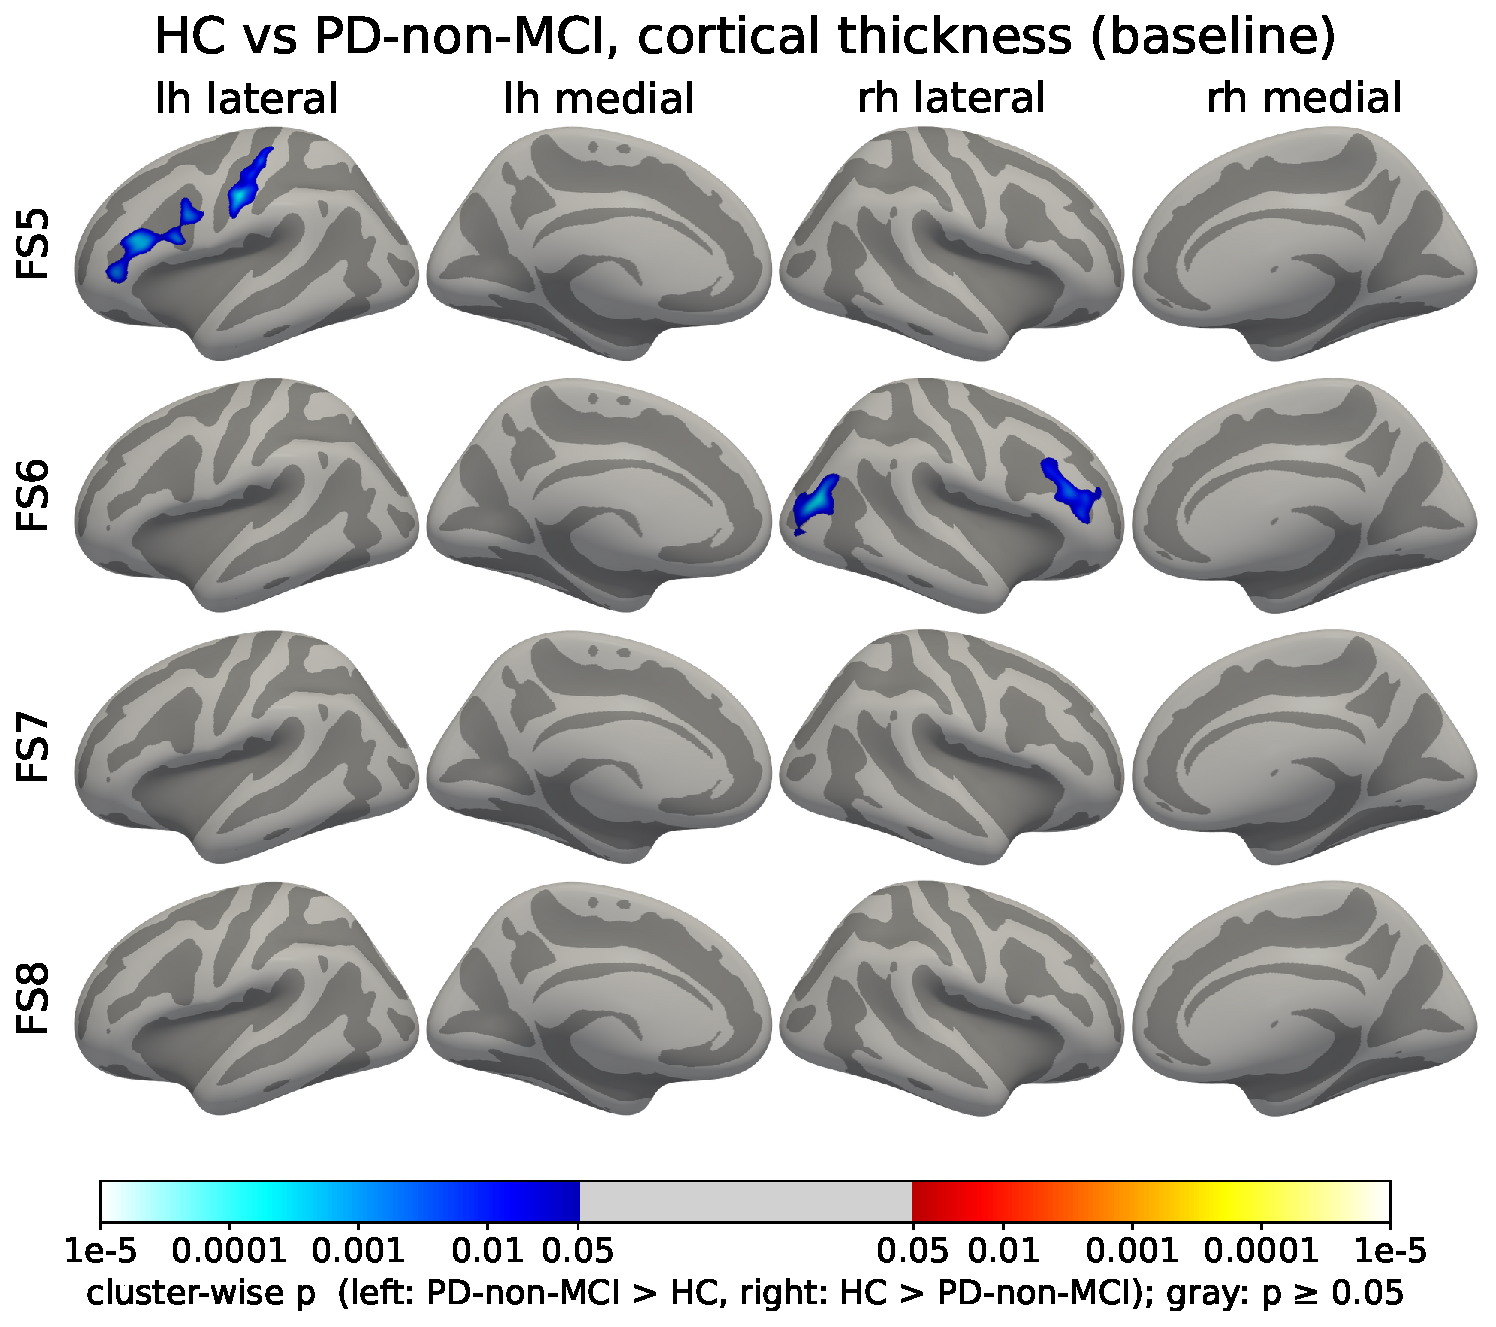
\includegraphics[width=\linewidth]{fig9_group_base}
\caption{Group differences (HC vs PD-non-MCI) in cortical thickness at baseline. Differences in FreeSurfer
\rev{7 and 8} were not significant.}\label{fig:9}
\end{figure}

\begin{figure}[H]
\centering
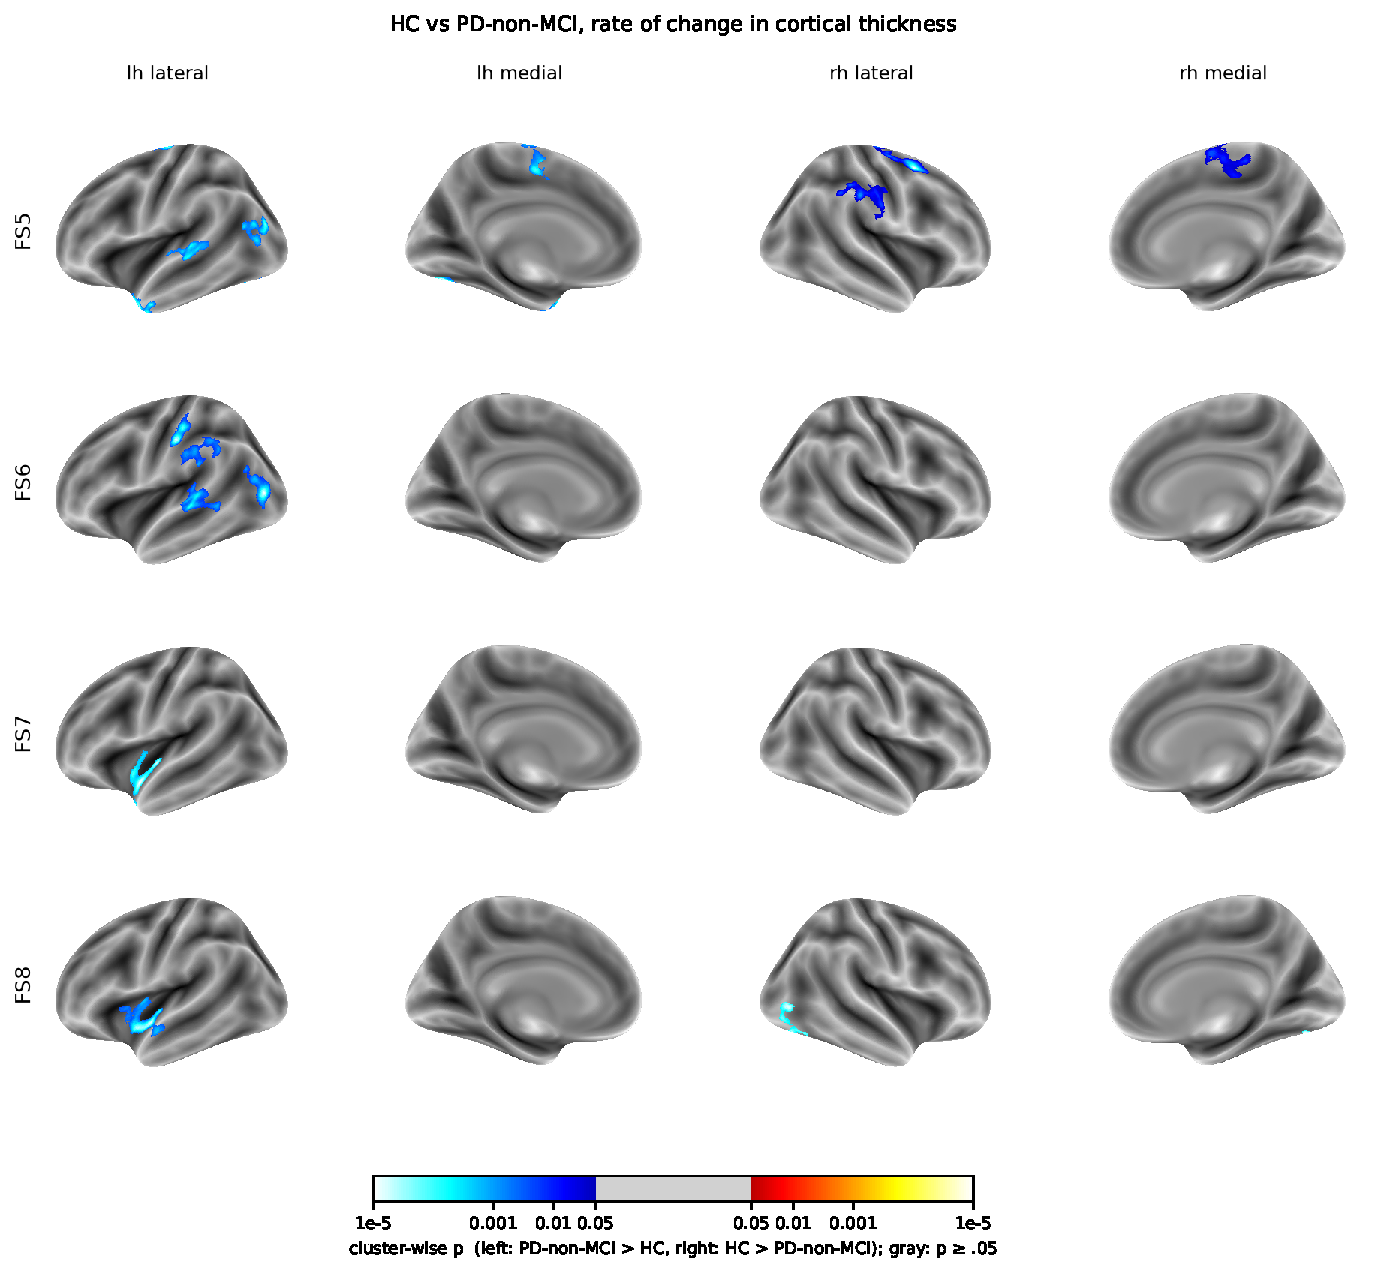
\includegraphics[width=\linewidth]{fig10_group_long}
\caption{Group differences (HC vs PD-non-MCI) in the rate of change in cortical thickness.}\label{fig:10}
\end{figure}

\rev{\subsection{Desikan--Killiany atlas}

With the bilateral Desikan--Killiany measures (34 cortical regions; mean thickness and volume, summed surface area),
the versions differed in 82\% (FS8 vs FS7) to 100\% (FS8 vs FS5) of the regions for thickness, 62\% (FS8 vs FS7) to
91\% (FS8 vs FS5) for surface area, and 81\% (FS7 vs FS6) to 96\% (FS8 vs FS5) for volume (cortical and
subcortical), so the larger regions of this atlas did not reduce the share of regions affected. FS8 and FS7 were
again the closest pair for surface area and thickness, mostly through the frontal, parietal and occipital regions
(40--50\% of these regions differed in surface area, against all insular and temporal regions). PD and HC did not differ in software variability (1 of 846 tests). In the clinical analyses,
one cingulate region per version differed between PD-non-MCI and HC in baseline volume (posterior cingulate in FS5,
caudal anterior cingulate in FS6--8), and FS7 and FS8 also found the caudal anterior cingulate in surface area. In
the rate of change, the pars opercularis differed in surface area in every version, with the middle temporal gyrus
added in FS7 and FS8 and the pars triangularis in FS8; the volume of the lingual gyrus (FS6) and of the fusiform
gyrus (FS7) differed in one version each. No version found a difference in thickness, and no region correlated with
UPDRS-III after correction ($\alpha = 0.05/34$).}

\rev{\subsection{Accuracy against manual labels (Mindboggle-101)}

All four versions processed the 101 Mindboggle-101 images. Agreement with the manual DKT31 labels decreased slightly
but consistently from the oldest to the newest version (Figure~S7): the mean Dice per image was 0.838 (SD 0.023) in
FS5, 0.829 (0.030) in FS6, 0.823 (0.029) in FS7 and 0.816 (0.029) in FS8 with the DKT parcellation, and 0.796,
0.784, 0.780 and 0.774 with the DK parcellation. In every version pair, the newer version had a lower Dice than the
older one ($p < 0.001$ for all 12 tests); FS8 was below FS5 in 100 of the 101 images (DKT) and in all 101 (DK),
by 0.022 on average. Region by region, FS8 had a lower Dice than FS5 in 54 of the 62 regions with the DKT
parcellation (50 with DK) and a higher one in none (2 with DK); FS7 and FS6 were the closest pair (18 regions lower
and one higher with DKT, 13 lower with DK). The largest decreases from FS5 to FS8 were in the entorhinal ($-0.05$),
pericalcarine ($-0.04$ to $-0.05$), caudal anterior cingulate and parahippocampal ($-0.04$) regions, while the pars
triangularis (both hemispheres) and the right pars opercularis and pars orbitalis did not change (DKT). The decrease
was found in every lobe and in every Mindboggle-101 sub-dataset with more than one image. Region volumes were
slightly overestimated in every version (median relative error $+0.2$ to $+3.8$\% with the DKT parcellation), with
a median absolute error of 7.5\% (FS5) to 8.6\% (FS6).}

\rev{\subsection{Repeat runs and computing environment}

Re-running a version on the same input reproduced its measures exactly, with a few exceptions in FS8. For FS5, FS6
and FS7, every aseg and Destrieux value of the 20 images (as written in the FreeSurfer stats files) was identical
in the two replicas and in the original run, although the original runs were made on another cluster. For FS8, the two replicas were identical, and 16 of the 20 images were identical
to the original run; in the 4 others, only two subcortical volumes differed, by at most 0.0005\% (5 of the 9,540
values compared). The original FS8 runs were also made on Rorqual. On the same images, the median
difference between versions was 1.4--3.5\% for thickness and 3.3--9.7\% for cortical volume, surface area and
subcortical volumes (labels that FS8 does not produce or defines differently left out of the FS8 pairs). For one image, the two FS6 replicas were stopped after 43~h while \texttt{mris\_fix\_topology} was still correcting
a very large left-hemisphere defect; this step had taken 66~h in the original run (73~h in total), so the image was
left out of the FS6 comparisons.}

\section{Discussion}

\note{Discussion: numbers updated for the revised sample; FS8 and image-quality paragraphs added (blue).}

This study investigated the impact of software variability resulting from FreeSurfer version updates on the
estimation of MRI-derived structural brain measures and the impact of this measurement variability on the
relationships between brain measures and clinical outcomes in Parkinson's disease. We observed variability across
many brain regions in the estimation of volume, surface area, and cortical thickness. The differences were more
wide-spread when comparing FS5 to the newer FreeSurfer versions while the differences between FS7 and FS6 were less
prevalent, although were still common. \rev{The differences between FS8 and FS7 were the least prevalent for surface
area and cortical thickness.} Our results are in line with previous research on FreeSurfer software variability
(Bhagwat et al., 2021; Gronenschild et al., 2012; Haddad et al., 2023) although these studies focused on different
FreeSurfer release versions. Relatively higher similarity between FS7 and FS6 in our study is in line with results
reported by Haddad et al. (2023) who report the lowest compatibility with FS5. Our data support the notion that the
choice of the software version may impact the estimation of structural measures. Importantly, not all regions were
equally impacted by the software variability and we found no differences in some of the regions. Volume estimation
of subcortical structures was relatively \rev{less} impacted by the variability between FS7 and FS6 which is in
line with Haddad et al. (2023). This could suggest that researchers focusing solely on these structures or volume
measures should not worry about the choice of the software. However, we refrain from such recommendations since
there is no clear pattern of regions that are less susceptible to the variability.

\rev{FS8 differed from FS7 less than any other pair for cortical measures, and nearly as much as FS5 differed from
FS6 and FS7 for subcortical structures. Surface area differed between FS8 and FS7 in 50.7\% of the regions and
cortical thickness in 72.3\%, the lowest proportions of the six pairs, and the median Sørensen--Dice coefficient of
the cortical labels was highest for this pair (.88, against .80 -- .87 for the other pairs). Subcortical volumes,
in contrast, differed in 31 of the 33 structures that both versions segment, and the mean Dice coefficient of the
14 subcortical structures of Tables~\ref{tab:2} and~\ref{tab:3} was .84 for each pair that includes FS8, against .91
between FS7 and FS6 and .81 between FS5 and FS6 or FS7 (Figure S4). The lowest overlaps between FS8 and FS7 were
for the accumbens area (.70 -- .73) and the pallidum (.77 -- .79). FS8 also no longer labels the vessels, the
choroid plexus, the optic chiasm and the 5th ventricle, so these structures cannot be compared with earlier
versions and their volumes cannot be carried over in longitudinal or multi-version studies.}

The impact of software variability on the estimation of all three structural measures is the same in patients
with PD and HC as we did not find any differences between these two groups \rev{(one region out of 2,898 tests)}.
It suggests that the variability introduced by different preprocessing toolboxes might also be present in other
cohorts. This result supports the fact that existing software variability results (such as Botvinik-Nezer et al.,
2020; Filip et al., 2022; Gronenschild et al., 2012) could also apply to the PD populations similar to the PPMI and
QPN samples tested in our study.

\rev{Differences in image quality between the groups do not explain this result. PD and HC images differed in
eight of the ten MRIQC metrics before correction for multiple comparisons; PD images had a lower coefficient of
joint variation and higher contrast-to-noise and signal-to-noise ratios, that is, slightly better image quality,
but also a higher Mortamet's quality index 1. Adjusting the group comparison of software variability for the total
signal-to-noise ratio and the scanner manufacturer left it unchanged (one significant test out of 2,898 without the
covariates, three with them). Image quality was nevertheless associated with software variability within the
sample: the coefficient of joint variation and the contrast-to-noise ratio correlated with the differences between
versions in 152 and 143 of the 888 thickness tests ($|r| \le .38$), and the gray-matter and total signal-to-noise
ratios had the strongest correlations, with volume differences ($|r|$ up to .62). Software variability therefore depends on image quality at the level of
individual images, while the two groups have similar variability once their images are compared directly. This
agrees with Sanz-Robinson et al. (2023), who found no correlation between data quality and the difference between
FreeSurfer and FSL hippocampal volumes, and it may not hold in populations with markedly lower image quality (e.g.,
children or patients with more severe motor symptoms).}

\rev{Image quality and scanner matter more for the clinical analyses than for software variability. The scanner
manufacturer differed between the clinical groups ($\chi^2 = 10.6$, $p = .005$; 17 PD-non-MCI and 3 HC scanned on
Philips systems). With the signal-to-noise ratio and the manufacturer as covariates, the subcortical results were
largely unchanged (Table S7), but the vertex-wise group differences in the rate of change in thickness almost
disappeared: one cluster remained in FS5 and none in FS6, FS7 or FS8 (Table S8). Part of these longitudinal
differences may therefore reflect acquisition differences between the groups rather than disease, independently of
the FreeSurfer version.} \note{PPMI acquisition site is not available in our study files; the manufacturer stands in
for it (Methods).}

To test the impact of software variability in a clinical setting, we investigated the differences between
FreeSurfer versions in the testing of clinical hypotheses. We tested group differences (patients vs healthy
participants) in subcortical volumes and cortical thickness as well as the correlation between disease severity in
patients and their cortical thickness. These hypotheses were derived from prior neuroimaging studies on PD (Hanganu
et al., 2014; Mak et al., 2015; for review see Mitchell et al., 2021). To our knowledge this is the first attempt
to assess the degree of impact of software variability on clinical findings in the PD population.

The significance of the differences between PD and HC in the estimation of the subcortical volumes was impacted by
software variability. The Sørensen--Dice coefficient of subcortical volumes between FS versions ranged from
\rev{.57 to .86}. Inconsistent results are in line with the study by Filip et al. (2022) who reported variability
across FS versions in the group differences in volume estimation in patients with diabetes. \rev{The significant group differences were larger subcortical volumes in PD-non-MCI than in HC, the opposite of the atrophy reported in PD (Mitchell et al., 2021). This direction did not depend on the version, and it held after adjusting for intracranial volume, image quality and scanner manufacturer. It may reflect the composition of this sample of early PD patients (67\% men against 48\% in HC, larger intracranial volume) rather than a disease effect, and the clinical analyses of this study were not designed to establish it. Our question was whether different versions reach the same conclusion:} various research teams, addressing the same clinical question, may or may not obtain significant results depending on the software they use. We have also found a significant correlation between the baseline volume of the right putamen
and the disease severity in \rev{one FS version (FS6), with p-values just above the corrected threshold in FS5 and
FS7.} \note{The submitted text linked the FS5 result to the FS5 differences in putamen volume; FS5 is no longer the
exception.} There are prior studies that indicate the link between the putamen volume and disease severity in PD
(Mak et al., 2014; Wilson et al., 2019).

\rev{The subcortical segmentation of FS8 had the largest effect on the clinical results. The Sørensen--Dice
coefficients of the significant group differences at baseline were lowest for the pairs that include FS8 (.57 with
FS5 and FS7, .67 with FS6): the bilateral thalamus was significant in every version, but FS8 was the only version
to detect the left accumbens area and the only version not to detect the right hippocampus. In the
longitudinal analysis, FS8 was the only version with a significant group difference in the left caudate. At the
vertex level, FS8 and FS7 agreed more closely: both found two baseline clusters of correlation with disease
severity, each including the left sensorimotor cortex (left postcentral gyrus in FS8, left precentral gyrus in
FS7), neither found a baseline group difference, and both found a group difference in the rate of change in thickness
of the left superior temporal gyrus. The longitudinal correlation with disease severity was significant in two right
hemisphere clusters (precuneus and middle temporal gyrus) in FS8 only. Agreement between two versions on cortical
measures therefore did not imply agreement on the clinical results, and the version with the most recent
segmentation methods changed the subcortical findings the most.}

Vertex-wise analyses yielded different results depending on the FS version. There was a correlation between the
disease severity and cortical thickness in numerous regions in FS5, a few in FS6, and only \rev{two significant
clusters in FS7 and in FS8}. This is not surprising given previous reports showing that FS5 is often less stringent
than more recent versions (Filip et al., 2022; Haddad et al., 2023).

\rev{FS5 and FS6 reported group differences between HC and PD-non-MCI in cortical thickness at baseline, FS7 and
FS8 did not.} This again would support the notion that \rev{older versions are} more permissive. This was also
observed in the longitudinal rate of change in cortical thickness where FS5 gave more significant regions than the
other \rev{three} FS versions. \note{The submitted text compared the left superior temporal clusters of FS6 and
FS7 (posterior vs anterior, no overlap); the left superior temporal gyrus is now found in all four versions: check
the overlap on the maps (Figure~\ref{fig:10}) and update.} Furthermore, reporting regions' labels is not sufficient
to determine similarity between the output.

\rev{To relate the differences to the software, we compared the programs and atlases each version ran at each
step of \texttt{recon-all} in our runs with the release notes (Table S39). The three transitions differ in kind.
FS5 to FS6 kept the same programs but retrained every atlas: the subcortical atlas used for skull stripping and
segmentation, the spherical folding atlas, and the three cortical parcellation atlases. This is consistent with
FS6 and FS5 being the pair with the most thickness differences, and with the changes in small subcortical labels
such as the 5th ventricle. FS6 to FS7 replaced bias-field correction (N3 by N4), added denoising before the white
surface and replaced the surface placement program (\texttt{mris\_make\_surfaces} by \texttt{mris\_place\_surface},
with remeshing and a pial surface pinned to the white surface in the medial wall), with a new subcortical atlas;
these changes act on the surfaces from which area and thickness are computed. The transition from FS7 to FS8 changed the steps that precede surface reconstruction. In our
runs, FS8 replaced the watershed skull stripping by SynthStrip (Hoopes et al., 2022), the Talairach registration
by SynthMorph (Hoffmann et al., 2022), and the atlas-based subcortical labeling (\texttt{mri\_ca\_register} and
\texttt{mri\_ca\_label}) by SynthSeg (Billot et al., 2023), and it added deep-learning segmentations of the dura,
the venous sinuses and the entorhinal white matter to guide pial surface placement. The surface placement program
(\texttt{mris\_place\_surface}), the spherical registration atlas and the cortical parcellation atlases are the
same as in FS7. This division matches our results: FS8 departs from FS7 mainly in subcortical volumes, which depend
on the replaced segmentation, while surface area and thickness, computed with the same surface and parcellation
tools, show the fewest differences of the six pairs. The cortical differences that remain between FS8 and FS7 may
come from the new skull stripping and the deep-learning guidance of the pial surface, which act before surface
placement.} \rev{In FS8, the subcortical segmentation from which the volumes are computed
(\texttt{aseg.auto\_noCCseg.mgz}) is the SynthSeg output itself; \texttt{mri\_ca\_label} is not run.}

Our study comes with limitations. We investigated one release of the major FS versions. Testing more versions,
including minor releases, could provide more insight into software variability, whether there are differences
between minor releases, and what could be the causes for the observed differences. Importantly, our study does not
provide information on analytical accuracy. Reported data shows that there are differences in the estimation of
structural metrics between FS versions, however, it is not possible to conclude from our data which version is
more accurate. \rev{Moreover, the clinical consequences of the measurement differences were limited to the
analyses where the group differences or correlations were close to the significance threshold: the group
differences between PD-non-MCI and HC in subcortical volumes were significant in the bilateral thalamus in every
version, and differed between versions only for structures with weaker effects. Whether these measurement differences change conclusions in PD studies with larger effects (e.g., later disease
stages or PD with dementia) remains to be tested.} \rev{The comparison with the manual labels of Mindboggle-101
partly addresses the question of accuracy, for the cortical parcellation: newer versions were not closer to the
manual labels, and the agreement decreased slightly from FS5 to FS8 (mean Dice 0.838 to 0.816). This decrease is
small compared with the differences between images (SD of the mean Dice about 0.03) but systematic, and it was
found with both the DKT and the DK parcellations, so it is not explained by the FS5 DKT atlas having been built from
Mindboggle-101 images. It does not mean that the measures of newer versions are less valid: the manual labels follow
one protocol, the atlases of FS6 and later were retrained on other images, and the regions where agreement
decreased most (entorhinal, parahippocampal, pericalcarine) have boundaries that depend strongly on the labelling
protocol. No manual subcortical reference was available in this dataset, so the accuracy of the subcortical
volumes, which carried the clinical results, remains untested.} \rev{The repeat runs show that the differences
between versions reported here do not come from re-running the analyses or from the computing environment: with the
same container and input, FS5--7 gave identical measures on two clusters, and FS8 differed from its original run
only in two subcortical volumes of 4 of the 20 images, by at most 0.0005\%. Running each version in a fixed container therefore made its results
reproducible across the clusters used here; this need not hold on hardware or operating systems with different
numerical behaviour.}

In conclusion, our results show that the variability across FreeSurfer versions impacts clinical results in the
studied PD populations at both subcortical volumetric and vertex-wise levels. The results differed even though we
used the same sample as well as the same preprocessing and statistical pipeline. Importantly, estimation of
structural metrics is impacted by software variability regardless of the sample with similar results across
patients with PD and HC. Observed variability is most likely not reserved solely to FreeSurfer since previous
studies reported variability in other analytical software. Our recommendation to users is to facilitate the latest
available release of the toolbox unless there is a particular reason to use another release. The most recent
software versions usually have improved algorithms and fixed issues discovered in previous releases which ensures
staying in line with current standards in the ever-changing field of neuroscience. \rev{The FS8 results qualify this recommendation for subcortical volumes: a study that
moves from FS7 to FS8 should expect changes of its subcortical findings larger than those of its cortical
findings.} Software versions should not be
updated during studies as it might introduce additional variability to the experiment.

\rev{FreeSurfer's release notes list the methodological changes of each version, and its mailing list supports
past releases, but neither quantifies how a change affects the measures. Releasing, with each version, the
differences in regional measures on a fixed reference dataset (for example, the PPMI images analyzed here) would
let users anticipate the effect of an update on their own analyses; numerical variability tests such as those of
Chatelain et al. (2023) could separate these effects from numerical noise.} Future studies may
also implement a multiverse approach to investigate clinical questions with several different software releases.

\section*{Acknowledgments}
This work was funded by the Michael J. Fox Foundation for Parkinson's Research (MJFF-021134). Computational analyses
were performed on the Narval \rev{and Rorqual clusters} hosted at Calcul Québec and part of Digital Research
Alliance of Canada.

\section*{Supplementary material}
\rev{Supplementary figures S1--S4 and tables S1--S8 are in the supplementary file; Tables S9--S28 (correlations
between MRIQC metrics and software variability) are provided as CSV files.}

\section*{References}
\begingroup\small\setlength{\parindent}{0pt}\setlength{\parskip}{0.5ex}
Bhagwat, N., Barry, A., Dickie, E. W., Brown, S. T., Devenyi, G. A., Hatano, K., ... \& Poline, J. B. (2021). Understanding the impact of preprocessing pipelines on neuroimaging cortical surface analyses. GigaScience, 10(1), giaa155.

\rev{Billot, B., Greve, D. N., Puonti, O., Thielscher, A., Van Leemput, K., Fischl, B., Dalca, A. V., \& Iglesias, J. E. (2023). SynthSeg: Segmentation of brain MRI scans of any contrast and resolution without retraining. Medical Image Analysis, 86, 102789.}

Botvinik-Nezer, R., Holzmeister, F., Camerer, C. F., Dreber, A., Huber, J., Johannesson, M., ... \& Rieck, J. R. (2020). Variability in the analysis of a single neuroimaging dataset by many teams. Nature, 582(7810), 84-88.

Bowring, A., Maumet, C., \& Nichols, T. E. (2019). Exploring the impact of analysis software on task fMRI results. Human brain mapping, 40(11), 3362-3384.

Chatelain, Y., Tetrel, L., Markiewicz, C. J., Goncalves, M., Kiar, G., Esteban, O., ... \& Glatard, T. (2023). A numerical variability approach to results stability tests and its application to neuroimaging. arXiv preprint arXiv:2307.01373.

\rev{Chatelain, Y., Sokolowski, A., Sharp, M., Poline, J.-B., \& Glatard, T. (2026). The practical impact of numerical variability on structural MRI measures of Parkinson's disease. Scientific Reports. https://doi.org/10.1038/s41598-026-64679-2}

Chougar, L., Faouzi, J., Pyatigorskaya, N., Yahia‐Cherif, L., Gaurav, R., Biondetti, E., ... \& Lehéricy, S. (2021). Automated categorization of parkinsonian syndromes using magnetic resonance imaging in a clinical setting. Movement Disorders, 36(2), 460-470.

Filip, P., Bednarik, P., Eberly, L. E., Moheet, A., Svatkova, A., Grohn, H., ... \& Mangia, S. (2022). Different FreeSurfer versions might generate different statistical outcomes in case–control comparison studies. Neuroradiology, 1-9.

Gaurav, R., Yahia‐Cherif, L., Pyatigorskaya, N., Mangone, G., Biondetti, E., Valabrègue, R., ... \& Lehéricy, S. (2021). Longitudinal changes in neuromelanin MRI signal in Parkinson's disease: a progression marker. Movement Disorders, 36(7), 1592-1602.

Ghosh, S. S., Poline, J. B., Keator, D. B., Halchenko, Y. O., Thomas, A. G., Kessler, D. A., \& Kennedy, D. N. (2017). A very simple, re-executable neuroimaging publication. F1000Research, 6.

Gomez-Ramirez, J., Quilis-Sancho, J., \& Fernandez-Blazquez, M. A. (2022). A comparative analysis of mri automated segmentation of subcortical brain volumes in a large dataset of elderly subjects. Neuroinformatics, 20, 63-72.

Gronenschild, E. H., Habets, P., Jacobs, H. I., Mengelers, R., Rozendaal, N., Van Os, J., \& Marcelis, M. (2012). The effects of FreeSurfer version, workstation type, and Macintosh operating system version on anatomical volume and cortical thickness measurements. PloS one, 7(6), e38234.

Haddad, E., Pizzagalli, F., Zhu, A. H., Bhatt, R. R., Islam, T., Ba Gari, I., ... \& Jahanshad, N. (2023). Multisite test–retest reliability and compatibility of brain metrics derived from FreeSurfer versions 7.1, 6.0, and 5.3. Human Brain Mapping, 44(4), 1515-1532.

Hanganu, A., Bedetti, C., Degroot, C., Mejia-Constain, B., Lafontaine, A. L., Soland, V., ... \& Monchi, O. (2014). Mild cognitive impairment is linked with faster rate of cortical thinning in patients with Parkinson’s disease longitudinally. Brain, 137(4), 1120-1129.

\rev{Hoffmann, M., Billot, B., Greve, D. N., Iglesias, J. E., Fischl, B., \& Dalca, A. V. (2022). SynthMorph: Learning contrast-invariant registration without acquired images. IEEE Transactions on Medical Imaging, 41(3), 543-558.}

\rev{Hoopes, A., Mora, J. S., Dalca, A. V., Fischl, B., \& Hoffmann, M. (2022). SynthStrip: Skull-stripping for any brain image. NeuroImage, 260, 119474.}

\rev{Klein, A., \& Tourville, J. (2012). 101 labeled brain images and a consistent human cortical labeling protocol. Frontiers in Neuroscience, 6, 171.}

Le, H., Zeng, W., Zhang, H., Li, J., Wu, X., Xie, M., ... \& Shen, J. (2020). Mean apparent propagator MRI is better than conventional diffusion tensor imaging for the evaluation of Parkinson’s disease: a prospective pilot study. Frontiers in Aging Neuroscience, 12, 563595.

Mak, E., Bergsland, N., Dwyer, M. G., Zivadinov, R., \& Kandiah, N. J. A. A. J. N. (2014). Subcortical atrophy is associated with cognitive impairment in mild Parkinson disease: a combined investigation of volumetric changes, cortical thickness, and vertex-based shape analysis. American Journal of Neuroradiology, 35(12), 2257-2264.

Mak, E., Su, L., Williams, G. B., Firbank, M. J., Lawson, R. A., Yarnall, A. J., ... \& O’Brien, J. T. (2015). Baseline and longitudinal grey matter changes in newly diagnosed Parkinson’s disease: ICICLE-PD study. Brain, 138(10), 2974-2986.

Masouleh, S., Eickhoff, S. B., Zeighami, Y., Lewis, L. B., Dahnke, R., Gaser, C., ... \& Valk, S. L. (2020). Influence of processing pipeline on cortical thickness measurement. Cerebral Cortex, 30(9), 5014-5027.

Mitchell, T., Lehéricy, S., Chiu, S. Y., Strafella, A. P., Stoessl, A. J., \& Vaillancourt, D. E. (2021). Emerging neuroimaging biomarkers across disease stage in Parkinson disease: a review. JAMA neurology, 78(10), 1262-1272.

Niso, G., Botvinik-Nezer, R., Appelhoff, S., De La Vega, A., Esteban, O., Etzel, J. A., ... \& Rieger, J. W. (2022). Open and reproducible neuroimaging: from study inception to publication. NeuroImage, 119623.

Rane, S., Plassard, A., Landman, B. A., Claassen, D. O., Donahue, M. J., \& Alzheimer’s Disease Neuroimaging Initiative. (2017). Comparison of cortical and subcortical measurements in normal older adults across databases and software packages. Journal of Alzheimer's disease reports, 1(1), 59-70.

Reuter M, Fischl B. Avoiding asymmetry-induced bias in longitudinal image processing. Neuroimage. 2011;57(1):19–21.

Reuter M, Rosas HD, Fischl B. Highly accurate inverse consistent registration: A robust approach. Neuroimage. 2010;53(4):1181–96.

Reuter M, Schmansky NJ, Rosas HD, Fischl B. Within-subject template estimation for unbiased longitudinal image analysis. Neuroimage. 2012;61(4):1402–18.

Sanz-Robinson, J., Torabi, M., Wishard, T. J., Glatard, T., Poline, J. B. (2023). Is between-pipeline variability affected by image quality? [Conference presentation]. OBHM 2023, Montreal, QC, Canada. www.humanbrainmapping.org

Sarasso, E., Agosta, F., Piramide, N., \& Filippi, M. (2021). Progression of grey and white matter brain damage in Parkinson's disease: a critical review of structural MRI literature. Journal of neurology, 268, 3144-3179.

Tessa, C., Lucetti, C., Giannelli, M., Diciotti, S., Poletti, M., Danti, S., ... \& Toschi, N. (2014). Progression of brain atrophy in the early stages of Parkinson's disease: A longitudinal tensor‐based morphometry study in de novo patients without cognitive impairment. Human brain mapping, 35(8), 3932-3944.

Wilson, H., Niccolini, F., Pellicano, C., \& Politis, M. (2019). Cortical thinning across Parkinson's disease stages and clinical correlates. Journal of the Neurological Sciences, 398, 31-38.

\endgroup

\end{document}
